\documentclass[11pt,reqno]{amsart}
\usepackage[margin=1.05in]{geometry}
\usepackage{amsmath,amssymb,amsthm,mathtools,booktabs,longtable,array,enumitem}
\usepackage[hyphens]{url}
\usepackage[colorlinks=true,linkcolor=blue,citecolor=blue,urlcolor=blue]{hyperref}
\usepackage[expansion=false]{microtype}
\usepackage{graphicx}

\setlist{leftmargin=2em}
\emergencystretch=2em

\theoremstyle{plain}
\newtheorem{theorem}{Theorem}[section]
\newtheorem{proposition}[theorem]{Proposition}
\newtheorem{lemma}[theorem]{Lemma}
\newtheorem{corollary}[theorem]{Corollary}
\newtheorem*{theoremA}{Theorem A}
\newtheorem*{theoremB}{Theorem B}
\newtheorem*{theoremC}{Theorem C}
\newtheorem*{theoremD}{Theorem D}
\newtheorem*{corollaryBp}{Corollary B$'$}
\newtheorem*{propositionE}{Proposition E}
\theoremstyle{definition}
\newtheorem{definition}[theorem]{Definition}
\newtheorem{remark}[theorem]{Remark}
\newtheorem{assumption}[theorem]{Assumption}

% Pointer to the script that produced a number
\newcommand{\cert}[2]{\par\smallskip{\raggedright\noindent\emph{Computation:} \texttt{#1}; output \texttt{#2}.\par}}

\newcommand{\R}{\mathbb R}
\newcommand{\hG}{h_\Gamma}
\newcommand{\hO}{h_\Omega}
\newcommand{\Gh}{\Gamma_h}
\newcommand{\Oh}{\Omega_h}
\newcommand{\Th}{\mathcal T_h}
\newcommand{\EG}{\mathcal E_h^\Gamma}
\newcommand{\Vh}{V_h}
\newcommand{\VR}{V_h^R}
\newcommand{\VO}{V_h^0}
\newcommand{\Pih}{\Pi_h}
\newcommand{\Zh}{Z_h}
\newcommand{\Wh}{W_h}
\newcommand{\gI}{g_I}
\newcommand{\dn}{\partial_n}
\newcommand{\dt}{\partial_\tau}
\newcommand{\ut}{\tilde u}
\newcommand{\pt}{\tilde p}
\newcommand{\ft}{\tilde f}
\newcommand{\psit}{\tilde\psi}
\newcommand{\pbar}{\bar p}
\newcommand{\pbG}{\bar p_{\Gamma}}
\newcommand{\ip}[2]{\langle #1,\, #2\rangle}
\newcommand{\tnorm}[1]{|\!|\!|#1|\!|\!|}
\newcommand{\norm}[1]{\lVert #1\rVert}
\newcommand{\GS}{\mathrm{GS}}
\newcommand{\CNS}{\mathrm{CNS}^\ast}
\newcommand{\eps}{\varepsilon_h}
\newcommand{\curl}{\operatorname{curl}}
\renewcommand{\div}{\operatorname{div}}
\newcommand{\Rc}{\mathcal R}
\newcommand{\Gc}{\mathcal G}
\newcommand{\cS}{\mathcal S}
\DeclareMathOperator{\diam}{diam}
\DeclareMathOperator{\dist}{dist}

\begin{document}

\title[Scott--Vogelius--Nitsche on polygonal boundaries]{Scott--Vogelius--Nitsche on a polygonally approximated boundary: convergence, the missing pressure traction, and the penalty threshold}
\author{Jaideep Sai Padhi}
\address{Department of Computer Science, Purdue University, West Lafayette, IN 47907, USA}
\email{jpadhi@purdue.edu}
\date{\today}
\subjclass[2020]{Primary 65N30; Secondary 65N12, 65N15, 76D07}
\keywords{Stokes equations, Scott--Vogelius elements, Nitsche's method, curved boundaries, divergence-free finite elements}

\begin{abstract}
We analyse the Scott--Vogelius--Nitsche method of Gjerde and Scott for two-dimensional Stokes flow whose no-slip curve is replaced by an inscribed polygon: continuous $P_k$ velocities ($k\ge4$) that are exactly divergence-free, with Dirichlet data imposed weakly on the polygon by Nitsche's method. This answers Scott's zero-gradient prize question, which asks whether the $H^1$ error behaves like $h_\Gamma^{3/2}+h_\Omega^k$ for general Stokes data and, if not, why not.

For the method as printed, the answer is no as soon as the pressure is not constant on the boundary. The printed Nitsche form omits the traction $-pn$. We prove that the method converges, at the sharp rate $h/\mu$ in the $H^1$ seminorm and at the exact rate $(h/\mu)^{1/2}$ in the mesh-dependent energy norm. To leading order the error is an explicit field: the discrete velocity leaks through the wall with normal velocity $(h/\mu)(p-\bar p)$, with constant exactly $1$ in the slip and energy norms. The $H^1$ rate is $1$ and not $1/2$ only because incompressibility turns the normal part of the missing traction into a tangential derivative.

The naive pressure-consistent correction is singular. A mean-corrected variant is well posed and attains $h_\Gamma^{3/2}+h_\Omega^k$ for general data and every fixed $k\ge4$, provided the boundary edges are not too short relative to the bulk mesh, using the Guzm\'an--Scott inf-sup constant made uniform over the perturbed domains.

We also show that the Nitsche penalty must scale like $\rho=h_\Omega/\min_e|e|$, with necessity certified in exact rational arithmetic. A computational study up to $N=256$ boundary chords confirms every rate and constant. It includes a pure-pressure test that isolates the traction response exactly, and a penalty study in which the threshold is linear in $\rho$ with slope about $20$.
\end{abstract}

\maketitle

\section{Introduction}\label{sec:intro}

\subsection*{Background}
\emph{Exactly divergence-free elements.} Scott and Vogelius \cite{ScottVogelius1985} showed that continuous piecewise-$P_k$ velocities with discontinuous piecewise-$P_{k-1}$ pressures satisfy $\div\Vh=\Pih$ for $k\ge4$ on meshes without singular vertices; the inf-sup constant was later made explicit in terms of the local mesh geometry \cite{GuzmanScott2019}. The discrete velocity is then divergence-free pointwise, not only weakly. This gives exact mass conservation. On fitted meshes with strongly imposed no-slip data it also gives pressure robustness: the velocity error does not depend on the pressure, which matters when pressure gradients are large or the viscosity is small \cite{JohnEtAl2017}. Split meshes give similar pairs of lower degree \cite{GuzmanNeilan2018}; see \cite{Neilan2020} for a review.

\emph{Curved walls.} Exact incompressibility has a cost at a curved wall. A divergence-free field that is smooth at a polygon vertex and vanishes on both adjacent edges has zero gradient there, and piecewise-polynomial divergence-free fields inherit such gradient constraints at the vertices of a polygonal wall \cite{ScottPrize,GjerdeScott2024}. If the wall is replaced by an inscribed polygon and no-slip is imposed strongly, the computed gradient can therefore be off by $O(1)$ at the polygon vertices, and the $H^1$ error of Scott--Vogelius elements then decays only like $h^{1/2}$ \cite{ScottPrize,GjerdeScott2024}, compared with $h^{3/2}$ for scalar problems \cite{BergerScottStrang1972,Scott1975}. How strongly this locking acts depends on the mesh at the wall, at least in our computations (Section~\ref{num:strong}). For a conforming piecewise-polynomial field the constraints at a wall vertex depend on its star: with two triangles they force a zero gradient, with three they leave a one-parameter family. On a mesh in which alternate polygon vertices lie in only two triangles we reproduce the rate $h^{1/2}$ with an $O(1)$ vertex-gradient error. On the meshes used in the rest of this paper, where every polygon vertex lies in three triangles, strong imposition shows no locking in the range computed ($H^1$ rates decreasing from $1.93$ to $1.61$ at $N=128$). We have not analysed strong imposition, and we do not claim that three triangles per wall vertex suffice in general; the observation suggests that the $h^{1/2}$ phenomenon needs wall vertices whose stars are singular or nearly singular.

One remedy is to fit the geometry, with isoparametric or Piola-mapped elements \cite{NeilanOtus2021,DurstNeilan2024}. Gjerde and Scott \cite{GjerdeScott2024} keep the polygon and impose the wall condition weakly by Nitsche's method \cite{Nitsche1971}, with penalty $\mu/h$ and no pressure term, and report errors orders of magnitude below those of strong imposition. Scott observed $H^1$ errors of order $h^{3/2}$ for this Scott--Vogelius--Nitsche method on a benchmark with constant pressure \cite{ScottPrize}. His zero-gradient prize \cite{ScottPrize} asks for a published proof that Scott--Vogelius--Nitsche converges, including a computational study of the influence of the Nitsche penalty. It states the expected error $\hG^{3/2}+\hO^k$ and adds: \emph{if this does not hold, why not?} We treat the question for general Stokes data.

\subsection*{Answer}
For the method as printed in \cite[(27)--(28)]{GjerdeScott2024} and bounded $\gamma$, the expected estimate holds if and only if the pressure is constant on the wall. The printed Nitsche form contains no traction term $-pn$. When $p$ varies along $\Gamma$, the penalty, not a traction, balances the pressure. The discrete velocity then leaks through the wall with normal velocity $(h/\mu)(p-\pbar)$, and the error is dominated by this leak (Theorems~A--C, Corollary~B$'$ and Theorem~B$''$). The mean-free correction $\CNS$ (cf.\ Frachon, Nilsson and Zahedi \cite{FrachonNilssonZahedi2024}), well posed for $\gamma\ge\gamma_2$, restores the expected rate (Theorem~D), and its $\hG^{3/2}$ term cannot be improved whenever the wall shear is not identically zero (Theorem~D$'$). On every mesh whose shortest boundary edge carries a triangle with apex angle at least $35^\circ$ and base angles at least $5^\circ$, the penalty threshold must grow with the ratio of bulk to boundary mesh size (Proposition~E).

\subsection*{Main results}
The notation is fixed in Section~\ref{sec:setting}. Throughout, $h=\hO$ is the bulk mesh size used in Scott's penalty $\mu/h$, $\hG$ is the length of the longest boundary edge, $\rho=h/\min_e|e|$, $\gamma=\mu\hG/h$ and $G=\norm{p-\pbar}_{L^2(\Gamma)}$. Constants do not depend on $h,\hG,\mu,\gamma$ or $\rho$.

\begin{theoremA}[Theorem~\ref{thm:A}]
The printed method $\GS$ converges, and its error in the mesh-dependent energy norm is
\[
\tnorm{\ut-u_h}\;\asymp\;(h/\mu)^{1/2}\,G\;+\;O\bigl((1+\gamma^{1/2})\hG^{3/2}+\eps\bigr),
\]
with matching upper and lower bounds.
\end{theoremA}

\begin{theoremC}[Theorem~\ref{thm:C}]
$\norm{\nabla(\ut-u_h)}\le C_p\,h/\mu+C\bigl((1+\gamma^{1/2})\hG^{3/2}+\eps\bigr)$.
The rate $1$ (rather than $1/2$) holds because $\div v=0$ turns the normal load into a tangential derivative (Lemma~\ref{lem:cancel}).
\end{theoremC}

\begin{theoremB}[Theorem~\ref{thm:B}]
In the regime where the pressure term dominates, the slip satisfies $\norm{\ut-u_h}_{L^2(\Gh)}\asymp (h/\mu)G$ and $\norm{\nabla(\ut-u_h)}\asymp h/\mu$. So Theorem~C is sharp.
\end{theoremB}

\begin{corollaryBp}[Corollary~\ref{cor:Bp}]
$\ut-u_h=(h/\mu)\,v_\varphi+o\bigl((h/\mu)^{1/2}\bigr)$ in the energy norm, where $v_\varphi$ is an explicit divergence-free field with $v_\varphi\approx-(p-\pbar)n$ on $\Gh$. In particular
\[
\frac{\norm{\ut-u_h}_{L^2(\Gh)}}{(h/\mu)G}\to1,
\qquad
\frac{\tnorm{\ut-u_h}}{(h/\mu)^{1/2}G}\to1.
\]
\end{corollaryBp}

\begin{theoremBpp}[Theorem~\ref{hc:thm}, Corollary~\ref{hc:cor}]
Let $U$ be the Stokes flow in $\Omega$ with Dirichlet data $-(p-\pbar)n$ on $\Gamma$ and $0$ on $\partial R$. For fixed $\gamma$ and bounded $\rho$, $(\mu/h)(\ut-u_h)\to U$ in $H^1$, so
\[
\frac{\norm{\nabla(\ut-u_h)}}{(h/\mu)G}\to K:=\frac{\norm{\nabla U}_{L^2(\Omega)}}{G}.
\]
The constant $K$ is not universal: it depends on the domain. For the pressure of our test P it is $K=2.7565157$ (series computation, inside a rigorous bracket $[2.0746,3.0526]$), and $K\to3/\sqrt7$ as the outer box grows. Convergence in the regime $\gamma\hG\to\infty$ is observed but not proved.
\end{theoremBpp}

\begin{theoremD}[Theorems~\ref{thm:D}, \ref{rs:unif} and~\ref{rs:Dfc}]
The naive consistent form, which adds $\ip{p_h}{v\cdot n}$, is singular; its $L^2_0$ variant is square but only gives $\div u_h\equiv c$, with $c\ne0$ in general (Proposition~\ref{prop:singular}). The mean-free correction $\CNS$, which adds $\ip{p_h-\pbG(p_h)}{v\cdot n}$ to the momentum row only, is well posed for $\gamma\ge\gamma_2$ and keeps $u_h$ exactly divergence-free; its velocity coincides with that of the zero-net-flux formulation of \cite{FrachonNilssonZahedi2024} (Remark~\ref{rem:fnz}). With the flux-corrected outer data $\tilde g_I$ of Definition~\ref{rs:def}, for general Stokes data, every fixed $k\ge4$ and every $\gamma\ge\gamma_2$,
\[
\norm{\ut-u_h}_{H^1(\Oh)}\le C\bigl(\hG^{3/2}+\hO^{k}\bigr),
\]
with $C$ independent of $\gamma$ and with no relation between $\hG$ and $\hO$. This is Scott's expected rate. With the plain interpolant $\gI$ the same holds under the proviso that the boundary edges are not too short relative to the bulk ($\hG\ge\hO^4$ for even $k$, $\hG\ge\hO^2$ for odd $k$); without it a single lower-order term, due to the net flux of the interpolated outer data, remains. On Clough--Tocher refinements the estimate of Theorem~\ref{thm:D} holds for every $k\ge2$ (Theorem~F).
\end{theoremD}

\begin{theoremDp}[Theorem~\ref{lb:thm}, Corollary~\ref{lb:cor}]
Suppose the wall shear $W=\dn u\cdot\tau$ is not identically zero. For $\CNS$, and for $\GS$ with any $G$,
\[
\norm{\nabla(\ut-u_h)}\ge c\,\norm{W}_{L^2(\Gamma)}\,\hG^{3/2}-C\hG^2 ,
\]
with $c$ independent of $\gamma,\mu,\rho$ and the pressure. So, whenever $\eps\le C\hG^{3/2}$ and $\gamma$ is bounded (or the data are flux-corrected and $\hO^k\le\hG^{3/2}$), the rate $\hG^{3/2}$ of Theorem~D (and of Theorem~A at $G=0$) is exact; it is the $\hG^{3/2}$ term, not the $\hO^k$ term, that is shown to be sharp. This is \emph{unconditional for $k\ge7$}. \emph{For $4\le k\le6$ it is conditional} on a local, scale-invariant condition (M3) on the boundary stars, which we have not proved; we verified it numerically at every boundary vertex of our meshes, for $N$ up to $1024$.
\end{theoremDp}

\begin{propositionE}[Proposition~\ref{prop:penalty}, Theorem~\ref{pb:thm}, Corollary~\ref{pb:rho}]
The condition $\mu\ge4\kappa C_I^2\rho$, $\rho=h/\min_{e\in\EG}|e|$, is sufficient for coercivity on every mesh. On every mesh, coercivity requires $\mu\ge\lambda_T\,h/|e|$ for each triangle $T$ with an edge $e$ on $\Gh$ (and not touching $\partial R$), with an explicit $\lambda_T$ depending only on the shape of $T$. In exact rational arithmetic, $\lambda_T>1$ whenever the apex angle is at least $35^\circ$ and $\lambda_T>9.3$ when it is at least $60^\circ$ (base angles at least $5^\circ$). So $\mu\gtrsim\rho$ is necessary on every mesh whose shortest boundary edge carries a triangle with apex angle at least $35^\circ$ and base angles at least $5^\circ$; for tall boundary triangles $\lambda_T<0$, and a necessity statement under (M0)--(M2) alone is open. Necessity is also certified on stars close to two reference stars.
\end{propositionE}

Theorem~A with $G=0$ gives $\tnorm{\ut-u_h}\le C((1+\gamma^{1/2})\hG^{3/2}+\eps)$. This recovers, for the printed method, the constant-pressure benchmark studied numerically in \cite{GjerdeScott2024,ScottPrize} and analysed in \cite{Cavalcante}, where the bound $\norm{u-u_h}_{H^1}\le C(\hO^k+\hG^{3/2})$ is proved for that benchmark, for fixed $k\ge4$ and also for $k\ge2$ on Clough--Tocher splits \cite[abstract and Cor.~5.3]{Cavalcante}. Our proof does not use \cite{Cavalcante}. Theorems~A--D$'$ hold for every fixed $k\ge4$ on meshes satisfying (M0)--(M2).

\subsection*{Further results}
\begin{theoremR}[Theorems~\ref{rs:unif}, \ref{rs:elower}, Corollaries~\ref{rs:rescue}, \ref{rs:rates}, Proposition~\ref{rs:cond}]
The $H^1$ error of the printed method is bounded uniformly in the penalty: $\norm{\nabla(\ut-u_h)}\le C_p\,\hG/\gamma+C(\hG^{3/2}+h^k+h^{\sigma_k}\hG^{-1/2})$ for every $\gamma\ge\gamma_0$. So a growing penalty $\mu\gtrsim h\hG^{-3/2}$ ($\mu\gtrsim h^{-1/2}$ when $h\asymp\hG$) restores the $H^1$ rate $\frac32$ of $\GS$ for general data. It cannot restore the energy norm: if $W\not\equiv0$ the energy error is at least $c\norm{W}\gamma^{1/2}\hG^{3/2}-C(\hG/\gamma)^{1/2}$ for large $\gamma$, so under a power-law penalty $\gamma\asymp\hG^{-\alpha}$ the energy rate of $\GS$ is $\min(\frac{1+\alpha}2,\frac{3-\alpha}2)\le1$ when $G>0$ and $W\not\equiv0$. The condition number of the velocity block grows by the factor $1+\gamma$, that of the pressure Schur complement by the factor $1+\mu/h$.
\end{theoremR}

\begin{theoremP}[Section~\ref{pd:sec}]
Let $p^\circ=\pt-\pbG(\pt)$. For $\CNS$ with flux-corrected data and $\gamma\in[\gamma_2,\gamma_{\max}]$, $\norm{p^\circ-p_h}_{L^2(\Oh)}\le C(\hG^{3/2}+\hO^k)$, including the constant, with $C$ depending on $\gamma_{\max}$ (Theorem~\ref{pd:thm:cnsp}). For $\GS$ the pressure is uniquely determined, but carries an explicit first-layer field $\xib$ produced by the symmetric Nitsche term acting on the leak; for fixed $\gamma$, bounded $\rho$ and $G>0$ the $L^2$ pressure error converges at the exact rate $\frac12$, and not at all pointwise in the first layer (Theorem~\ref{pd:thm:gsp}). The variational drag, lift and torque coincide with the integral of the Nitsche flux. For $\GS$ with fixed $\gamma$ and bounded $\rho$ their error is $-(h/\mu)\int_\Gamma(p-\pbar)(R_\psi-\bar R_\psi)+O(h^{3/2})$, with $R_\psi$ the pressure of a dual Stokes problem, so the rate is $1$ (Theorem~\ref{pd:thm:gsdrag}); for $\CNS$ with $\gamma\ge\max(1,\gamma_2)$ and $\gamma\hG\le1$ it is $O(\hG^2+\eps)$ (Theorem~\ref{pd:thm:cnsdrag}).
\end{theoremP}

\subsection*{Related work and what is new}
For Stokes, the consistent Nitsche form uses the full traction $\sigma(u,p)n$. It therefore contains the pressure term $\ip{p}{v\cdot n}$ \cite{FreundStenberg1995,Stenberg1995,Becker2002,BurmanHansbo2014}, and this term is recognised as essential for consistency \cite{BurmanHansboLarson2019Stokes}. The Gjerde--Scott form omits it. On the geometric side, boundary-value correction \cite{BrambleDupontThomee1972} has been combined with Nitsche's method for cut elements \cite{BurmanHansboLarson2018,BurmanHansboLarson2019Stokes} and for polygonal approximations of scalar problems \cite{DupontGuzmanScott2025}; the shifted boundary method \cite{MainScovazzi2018} is a related approach. None of these works uses exactly divergence-free spaces.
%% VERIFY: FreundStenberg1995 treats Stokes only per a secondary citation; Becker2002 content not read (notes/v5/lit_report.md).

With such spaces, the placement of the pressure term decides whether exact incompressibility survives. If the term also appears in the continuity equation, $\div u_h$ vanishes only away from an $O(h)$ boundary strip \cite{LiuNeilanOlshanskii2023}. If it appears only in the momentum equation, the constant pressure mode must be handled separately. Frachon, Nilsson and Zahedi \cite{FrachonNilssonZahedi2024} show that fixing the pressure mean by a Lagrange multiplier makes $\div u_h$ equal to that multiplier, and avoid this by testing the momentum equation only with velocities of zero net flux. Our $\CNS$ is this device in square form: its velocity coincides with theirs (Remark~\ref{rem:fnz}), and its wall-mean subtraction fixes the pressure constant automatically. The work closest to ours is that of Liu, Neilan and Otus \cite{LiuNeilanOtus2023}, for Scott--Vogelius elements on Clough--Tocher splits of a mesh inside a curved domain. They add a mean-free boundary multiplier that approximates the wall pressure up to a constant, together with a zero-flux constraint and a Taylor boundary correction. Their velocity is exactly divergence-free and converges at the optimal order $h^k$; without the constraint, they note, the method is ill posed \cite[Remark~3.2]{LiuNeilanOtus2023}. Related multiplier formulations for cut elements are given in \cite{BurmanHansboLarson2024}. Exactly divergence-free methods also require discrete Dirichlet data with zero net flux \cite{EickmannScottTscherpel2025}; our flux-corrected $\tilde g_I$ is a simple instance.

Our subject is the method as Gjerde and Scott printed it, and its minimal repair: no extra unknowns, no boundary correction, and the pressure itself on the wall. We do not claim the mean-free device as new. As far as we know, what is new is the analysis:
\begin{itemize}
\item the two-sided leak analysis of the printed method (Theorems~A--C, Corollary~B$'$), including the identification of its $H^1$ constant (Theorem~B$''$) and of its pressure and drag defects (Theorem~P);
\item the proof of Scott's conjectured rate $\hG^{3/2}+\hO^k$ for the mean-free correction on an inscribed polygon (Theorem~D), with the penalty-uniform $H^1$ bound, and the proof that its $\hG^{3/2}$ term is sharp (Theorem~D$'$);
\item the penalty threshold $\propto\rho$: sufficiency is a standard consequence of the trace-inverse inequality \cite{Stenberg1995,JuntunenStenberg2009}, while the explicit necessity certificates of Proposition~E appear to be new;
\item the extensions: Clough--Tocher refinements, general smooth domains, steady Navier--Stokes and three dimensions (Theorems~F--I), and the growing-penalty analysis (Theorem~R).
\end{itemize}
That the pressure term is needed for consistency is not new \cite{BurmanHansboLarson2019Stokes}; the mechanism of the leak is the classical consistency error of boundary penalty methods \cite{Babuska1973}, here acting only on the pressure and with vanishing penalty parameter $h/\mu$, which is why the method converges at all.

\subsection*{Scope and related variants}
We analyse the symmetric Nitsche form of \cite{GjerdeScott2024}. The leak comes from the missing pressure term, not from the symmetry of the viscous terms, so we expect it in nonsymmetric variants as well; we have not analysed these, nor penalty-free variants \cite{FreundStenberg1995,Burman2012,BoiveauBurman2016}. Nitsche's method with Robin-type data is treated in \cite{JuntunenStenberg2009}. Multiplier and boundary-correction methods \cite{LiuNeilanOtus2023,BurmanHansboLarson2024,BrambleDupontThomee1972,DupontGuzmanScott2025} reach higher order than $\hG^{3/2}$, at the price of extra unknowns or Taylor corrections.
A common alternative restricts the pressure to $L^2_0$ and adds the plain term $\ip{p_h}{v\cdot n}$, testing the continuity equation only with mean-zero pressures. Because $\div\Vh=\Pih$, this gives only $\div u_h\equiv c$ with $c|\Oh|=\int_{\partial\Oh}u_h\cdot n$ (Proposition~\ref{prop:singular}; compare \cite[(5.9)]{FrachonNilssonZahedi2024}). The constant vanishes exactly when the naive system is solvable, equivalently when the $\CNS$ pressure has zero mean on $\Gh$. With weak imposition nothing forces the flux through $\Gh$ to vanish, even for flux-corrected data, and in our computations $c\ne0$.
Our proofs use Scott--Vogelius elements with $k\ge4$, and $k\ge2$ on Clough--Tocher splits, in two dimensions (with a three-dimensional extension, Theorem~I). Other divergence-free families, and cut or unfitted meshes, are not treated. Gjerde and Scott also treat slip conditions by Nitsche's method \cite{GjerdeScott2022}; we have not examined that method.
%% VERIFY: GjerdeScott2022 full text not read; whether its slip-Nitsche form contains a pressure term is unknown (notes/v5/lit_report.md).

\subsection*{Extensions}
\begin{theoremF}[Theorem~\ref{ct:thm:main}, Proposition~\ref{ct:prop:penalty}]
On the Clough--Tocher refinement of any shape-regular mesh whose boundary edges have comparable lengths, Theorems~A--D, Corollary~B$'$ and the sufficiency part of Proposition~E hold for every $k\ge2$, with no angle or singular-vertex condition. For example, $\CNS$ satisfies $\norm{\ut-u_h}_{H^1}\le C(\hG^{3/2}+h^2)$ for $k=2$ if $\hG\ge h^4$. The penalty necessity is recertified exactly on split stars.
\end{theoremF}

\begin{theoremG}[Section~\ref{gd:sec}]
In two dimensions, Theorems~A--D and Corollary~B$'$ extend to a bounded connected domain whose curved boundary consists of finitely many closed smooth curves, convex or not, with a nonempty polygonal component $\Sigma$ on which the data are imposed strongly. The geometric lemmas use only $C^3$ curves; the results assume the regularity (R1) of the solution, which for generic $f$ requires $\Gamma\in C^{k+1,\alpha}$, and the results that use the leak test field assume $\Gamma\in C^{k+3}$. With several curved components, the correct pressure constant is the \emph{global} boundary mean. $\CNS$ needs one global correction, and a per-component correction is inconsistent.
\end{theoremG}

\begin{theoremH}[Section~\ref{ns:sec}]
For steady Navier--Stokes, assume the discrete linearisation at the exact solution is uniformly stable; we prove this under a small-data condition. Then $\GS$ converges at $H^1$ rate $h/\mu$ with the same leak (slip and energy constants $1$), and $\CNS$ attains $\hG^{3/2}+\hO^k$. No inflow/outflow correction of the convective term is needed for these statements.
\end{theoremH}

\begin{theoremI}[Theorem~\ref{td:main}]
In three dimensions, with an inscribed triangulated polyhedron, Theorems~A--D and Corollary~B$'$ hold with the same rates, assuming a uniform discrete inf-sup constant. That assumption is known for Alfeld (barycentric) splits with $k\ge3$, by the published split-mesh theory combined with a uniform Bogovski\u{\i} bound that we prove; we have not re-audited the published proofs for hidden domain dependence. Only a spherical obstacle is treated. Penalty necessity, sharpness and unsplit meshes remain open in 3D.
\end{theoremI}

\subsection*{Computations}
Section~\ref{sec:numerics} reports computations with up to $N=256$ boundary chords, mostly for $k=4$, with $k=5,6$ and Clough--Tocher $k=2,3$ in Section~\ref{sec:numv3}. They show the following.
\begin{itemize}
\item The $\CNS$ $H^1$ rate decreases monotonically to $3/2$, independently of the pressure, for $k=4,5,6$.
\item The printed method has rate $1$ whenever $G>0$.
\item On a pure-pressure test that isolates the traction response exactly, the slip and energy constants of Corollary~B$'$ approach $1$ for every element tested. For $k=4$ the $H^1$ constants approach the $K$ of Theorem~B$''$; that they do so also for $k=5,6$ and on Clough--Tocher refinements is observed, not proved.
\item In the penalty study, the coercivity threshold $\mu^\ast$ is linear in $h/\hG$ over more than a decade, with $\gamma^\ast=\mu^\ast\hG/h\approx18$--$21$ for $k=4$. It is larger for higher $k$ and on Clough--Tocher refinements.
\item Strongly imposed no-slip shows the $h^{1/2}$ locking on a mesh with two-triangle wall vertices but not on our production meshes, while $\GS$ and $\CNS$ are insensitive to the change of mesh (Section~\ref{num:strong}).
\item The pressure errors follow Theorem~P: rate $\to\frac32$ for $\CNS$, and rate $\to\frac12$ for $\GS$ when $G>0$, carried by the first layer (Section~\ref{pd:sec:num}).
\item A growing penalty behaves as Theorem~R predicts, and flux-corrected data remove the flux floor exactly (Section~\ref{rs:sec:num}).
\end{itemize}
All code, raw outputs and logs are in the accompanying repository (Appendix~\ref{app:repro}).

\subsection*{Organisation}
Section~\ref{sec:setting} fixes the setting. Sections~\ref{sec:geometry}--\ref{sec:erroreq} collect geometric and discrete tools and the error equation. Section~\ref{sec:printed} treats the printed method and identifies its $H^1$ constant. Section~\ref{sec:consistent} treats the pressure-consistent method, proves the lower bound, and treats flux-corrected data and a growing penalty. Section~\ref{pd:sec} treats the pressure, the boundary stress and drag. Section~\ref{sec:penalty} treats the penalty threshold. Sections~\ref{ct:sec}--\ref{td:sec} contain the extensions: Clough--Tocher refinements, general domains, Navier--Stokes and three dimensions. Section~\ref{sec:numerics} reports the computations.

\section{Setting, methods and assumptions}\label{sec:setting}

\subsection*{Domain}
Let $R=(-L,L)^2$ with $L>1$, let $D$ be the open unit disk, $\Omega=R\setminus\overline D$ and $\Gamma=\partial D$.
Let $P_h$ be a convex polygon with vertices on $\Gamma$, $\Gh=\partial P_h$ and $\Oh=R\setminus P_h$. Since $P_h\subset D$, we have $\Omega\subset\Oh$. The strip $S_h=\Oh\setminus\overline\Omega$ lies between each chord and its arc.

\subsection*{Mesh}
$\Th$ is a conforming triangulation of $\Oh$, and $\EG$ is its set of edges on $\Gh$. We use the parameters
\[
h=\hO:=\max_{T\in\Th}\diam T,\qquad
\hG:=\max_{e\in\EG}|e|,\qquad
\rho:=\frac{h}{\min_{e\in\EG}|e|},\qquad
\gamma:=\frac{\mu\hG}{h}.
\]
Here $h$ is the $h$ in Scott's penalty $\mu/h$, and $\gamma$ is the effective boundary penalty, so that $\mu/h=\gamma/\hG$.

\begin{assumption}\label{ass:mesh}\leavevmode
\begin{enumerate}[label=(M\arabic*),start=0]
\item Shape regularity, and $c_0\hG\le|e|\le\hG$ for all $e\in\EG$. Hence $\rho/h\le1/(c_0\hG)$. No quasi-uniformity is assumed; $\hG\ll h$ is allowed.
\item No vertex of $\Th$ is singular. A vertex is singular if it is an interior vertex whose incident edges lie on two lines, a boundary vertex with one incident triangle, or a boundary vertex whose incident edges lie on two lines.
\item[(M1$'$)] Every vertex of $\Gh$ has at least three incident triangles. The angle of $\Oh$ at a vertex of $\Gh$ is $\pi+O(\hG)$, so with two triangles $\Theta(z)=O(\hG)\to0$, contradicting (M2).
\item $\Theta(z):=\max_j|\sin(\theta_j+\theta_{j+1})|\ge\Theta_0>0$ at every vertex $z$, in the notation of Guzm\'an--Scott \cite{GuzmanScott2019}. At boundary vertices the wrap-around term is omitted.
\end{enumerate}
\textbf{(D)} $\ft$ is smooth and bounded on a fixed neighbourhood of $\overline\Omega$, $\ft=f$ on $\Omega$, and $h\le h_\ast$ is small (hence so is $\hG\le h$).
\end{assumption}

\subsection*{Spaces}
Fix $k\ge4$. $\Vh$ is the space of continuous piecewise-$P_k$ vector fields, $\VR:=\{v\in\Vh:v|_{\partial R}=0\}$ and $\VO:=\{v\in\Vh:v|_{\partial\Oh}=0\}$.
$\Pih$ is the space of discontinuous piecewise-$P_{k-1}$ functions and $\Zh:=\{v\in\VR:\div v=0\}$.
$\Wh:=\{z\in\Vh:z|_{\partial R}=\gI,\ \div z=0\}$, where $\gI$ is the $P_k$ Lagrange interpolant of $g$. Gjerde and Scott, and all computations in Section~\ref{sec:numerics}, use $k=4$.

\subsection*{Forms}
$n$ is the outward unit normal of $\Oh$ on $\Gh$ (pointing into $P_h$), and $\ip\cdot\cdot$ is the $L^2(\Gh)$ pairing. Let
\begin{align*}
a_h(u,v)&=\tfrac12(Du,Dv),\qquad Du=\nabla u+(\nabla u)^{\mathsf T},\\
N_h(u,v)&=a_h(u,v)-\ip{\dn u}{v}-\ip{u}{\dn v}+\frac{\mu}{h}\ip{u}{v},\qquad \dn u:=(\nabla u)n .
\end{align*}

\begin{definition}[Method $\GS$ {\cite[(28)]{GjerdeScott2024}}, as printed]
Find $u_h\in\Vh$ with $u_h|_{\partial R}=\gI$ and $p_h\in\Pih$ such that
\[
N_h(u_h,v)-(p_h,\div v)=(\ft,v)\quad\forall v\in\VR,\qquad (q,\div u_h)=0\quad\forall q\in\Pih.
\]
\end{definition}

\begin{definition}[Method $\CNS$]
As $\GS$, with momentum row
\[
N_h(u_h,v)-(p_h,\div v)+\ip{p_h-\pbG(p_h)}{v\cdot n}=(\ft,v),\qquad \pbG(q):=|\Gh|^{-1}\int_{\Gh}q .
\]
\end{definition}

\subsection*{Exact solution and extensions}
$(u,p)$ is smooth with $-\Delta u+\nabla p=f$ and $\div u=0$ in $\Omega$, $u|_\Gamma=0$ and $u|_{\partial R}=g$; note $-\div D(u)=-\Delta u$. The stream function $\psi$ with $u=\curl\psi=(\partial_y\psi,-\partial_x\psi)$ is single-valued because $u\cdot n=0$ on $\Gamma$.
Let $\psit$ be a smooth extension of $\psi$ to a neighbourhood of $\overline\Omega$ and $\ut:=\curl\psit$, so $\div\ut=0$. Let $\pt$ be a smooth extension of $p$. Then $F:=\ft+\Delta\ut-\nabla\pt$ vanishes on $\Omega$ and is supported in $S_h$.

\subsection*{Norms and constants}
For $v$ with traces on $\Gh$,
\[
\tnorm{v}^2:=\norm{\nabla v}_{\Oh}^2+\frac{\mu}{h}\norm{v}_{\Gh}^2+\sum_{e\in\EG}|e|\,\norm{\dn v}_{L^2(e)}^2 .
\]
This is used for discrete fields and for errors $\ut-z$; since $\ut$ is smooth, every trace exists. We write $G:=\norm{p-\pbar}_{L^2(\Gamma)}$, with $\pbar$ the mean of $p$ over $\Gamma$.

$C$ and $c$ depend on (M0)--(M2), $k$, $L$ and norms of $(u,p,\psit)$. They are independent of $h,\hG,\mu,\gamma,\rho$ unless displayed. $C_p$ is a constant that may also depend on $\norm{p-\pbar}_{W^{1,\infty}(\Gamma)}$. Where $G$ is tracked explicitly, ``$\delta$ small'' means $\delta\le\delta_0(C_p)$.

\section{Geometry}\label{sec:geometry}

\begin{lemma}[Chords]\label{lem:chords}
Let $e$ be a chord of length $\ell$ and $x\in e$. Then $\dist(x,\Gamma)\le\ell^2/8+O(\ell^4)\le\ell^2/4$.
Let $s$ be the signed arclength from the chord midpoint $m_e$, $x^\ast$ the nearest point of $\Gamma$, and $\tau_e$ the unit tangent of $e$. Then, up to a fixed orientation sign,
\[
n(x^\ast)-n_e=-s\,\tau_e+O(\ell^2).
\]
The arclength Jacobian of the radial projection $\Gh\to\Gamma$ is $1+O(\ell^2)$.
\end{lemma}

\begin{proof}
The sagitta is $1-\sqrt{1-\ell^2/4}=\ell^2/8+\ell^4/128+\cdots$. The normal at $x^\ast$ is the radial unit vector. Its angle differs from that of $n_e$ by the central angle to $x^\ast$, which is $s+O(s^3)$.
\end{proof}

\begin{lemma}[Uniform trace, Friedrichs and Korn]\label{lem:korn}
There are $C_{\mathrm{tr}},C_F,\kappa$, independent of $h$, such that every $v\in H^1(\Oh)^2$ with $v|_{\partial R}=0$ satisfies
\[
\norm{v}_{L^2(\Gh)}\le C_{\mathrm{tr}}\norm{\nabla v},\qquad
\norm{v}\le C_F\norm{\nabla v},\qquad
\norm{\nabla v}^2\le\kappa\,a_h(v,v).
\]
\end{lemma}

\begin{proof}
\begin{enumerate}
\item Write $\Gh$ in polar form as $r=\rho_h(\theta)$. On a chord with endpoint angles $\theta_m\pm\alpha$ we have $\rho_h=\cos\alpha/\cos(\theta-\theta_m)$. Hence $\norm{\rho_h-1}_\infty\le C\hG^2$ and $\norm{\rho_h'}_\infty\le C\hG$.
\item Let $\chi$ be smooth, with $\chi(1)=1$ and $\chi\equiv0$ outside a fixed collar in $\Omega$. Define $\Phi_h(r,\theta)=(r+\chi(r)(\rho_h(\theta)-1),\theta)$.
\item $\Phi_h$ maps $\Omega$ onto $\Oh$ and $\Gamma$ onto $\Gh$, is the identity near $\partial R$, and is bi-Lipschitz with $\norm{D\Phi_h-I}_\infty\le C\hG$ almost everywhere.
\item For $w=v\circ\Phi_h$ we have $D(w)=D(v)\circ\Phi_h+E$ with $|E|\le C\hG|\nabla v\circ\Phi_h|$.
\item On the fixed domain $\Omega$, $w$ vanishes on $\partial R$, a set of positive measure. So the first Korn inequality, the trace inequality and the Friedrichs inequality hold.
\item Changing variables back gives $\norm{\nabla v}\le C(\norm{D(v)}+\hG\norm{\nabla v})$; absorb the last term for $\hG\le h_\ast$. The other two inequalities transfer the same way.\qedhere
\end{enumerate}
\end{proof}

\begin{lemma}[Extension]\label{lem:ext}
$\norm{\ut}_{L^\infty(\Gh)}\le C\hG^2$, so $\norm{\ut}_{L^2(\Gh)}\le C\hG^2$. For $v\in\VR$, $|(F,v)|\le C\hG^2\norm{\nabla v}$.
\end{lemma}

\begin{proof}
The first bound follows from Lemma~\ref{lem:chords} and $\ut|_\Gamma=0$. For the second, apply a one-dimensional Poincar\'e inequality across strips of width at most $C\hG^2$, and use $|S_h|\le C\hG^2$, $\norm{F}_\infty\le C$ (by (D)) and Lemma~\ref{lem:korn}.
\end{proof}

\begin{lemma}[Wall structure]\label{lem:wall}
On $\Gamma$: $\nabla u=\dn u\otimes n$, $\dn u\cdot n=0$ and $(\nabla u)^{\mathsf T}n=0$.
\end{lemma}

\begin{proof}
The tangential derivatives vanish, and $\div u=n\cdot\dn u$.
\end{proof}

\begin{lemma}[Transposed-gradient term]\label{lem:transposed}
For $v\in\VR$,
\[
|\ip{(\nabla\ut)^{\mathsf T}n}{v}|\le C\sum_{e\in\EG}\bigl(|e|^2\norm{v}_{L^1(e)}+|e|^2\norm{\dt v}_{L^1(e)}\bigr)\le C\hG^{3/2}\norm{\nabla v}.
\]
\end{lemma}

Pointwise the transposed term is only $O(\hG)$ on $\Gh$, not $O(\hG^2)$: although $\ut=O(\hG^2)$ there, the chord normal $n_e$ is tilted by $O(\hG)$ against $n(x^\ast)$ (step~1 below). The rate $\hG^{3/2}$ comes from the odd symmetry of the leading term in $s$ (step~2), not from the size of $\ut$. In the energy dual it can also be obtained from the penalty alone, $|\ip{(\nabla\ut)^{\mathsf T}n}{v}|\le C\hG\norm{v}_{\Gh}\le C\gamma^{-1/2}\hG^{3/2}\tnorm v$ (Lemma~\ref{pd:lem:G}); in the plain $H^1$ dual, without odd symmetry, it would be only $O(\hG)$.

The rate $\hG^{3/2}$ is sharp on $\VR$: a first-layer field with odd trace on each chord attains it, and the dual-norm test of Section~\ref{sec:numerics} gives $1.56$--$1.57$. For the method itself, which is tested on $\Zh$, Theorem~\ref{lb:thm} proves the matching lower bound $c\,\hG^{3/2}$ for the $H^1$ error, by a different route (unconditionally for $k\ge7$, and under a local condition on the boundary stars for $4\le k\le6$). The $\CNS$ $H^1$ rates of Table~\ref{tab:cns} decrease monotonically toward $3/2$. Lemma~\ref{lem:transposed} is a sharper dual-norm statement than the upper bounds need: by Remark~\ref{td:nocancel2d}, Lemma~\ref{lem:Gbound} and Theorems~\ref{thm:C} and~\ref{thm:D} also follow from the cruder energy-dual bound that holds without the odd-in-$s$ cancellation.

\begin{proof}
\begin{enumerate}
\item Taylor-expand about $x^\ast$ and apply Lemmas~\ref{lem:chords} and~\ref{lem:wall}:
\[
(\nabla\ut(x))^{\mathsf T}n_e=n(x^\ast)\bigl(\dn u(x^\ast)\cdot(n_e-n(x^\ast))\bigr)+O(\hG^2)=s\,a_e+O(\hG^2),
\]
where $a_e:=n(m_e^\ast)\bigl(\dn u(m_e^\ast)\cdot\tau_e\bigr)$ is constant on $e$. The $O(\hG^2)$ remainder collects $|x-x^\ast|$, the $O(\ell^2)$ term of Lemma~\ref{lem:chords}, and $s\cdot O(s)$.
\item Since $\int_e s\,ds=0$,
\[
\Bigl|\int_e s\,a_e\cdot v\Bigr|=\Bigl|\int_e s\,a_e\cdot(v-v(m_e))\Bigr|\le\frac{|e|^2}{4}\norm{\dt v}_{L^1(e)} .
\]
\item Use $\norm\cdot_{L^1(e)}\le|e|^{1/2}\norm\cdot_{L^2(e)}$ and the inverse trace inequality $|e|\norm{\dt v}^2_{L^2(e)}\le C_I^2\norm{\nabla v}^2_{T_e}$.
\item Summing, $\sum_e|e|^{5/2}\norm{\dt v}_{L^2(e)}\le C\hG^2(\#\EG)^{1/2}\norm{\nabla v}\le C\hG^{3/2}\norm{\nabla v}$. The zeroth-order term is handled the same way, finishing with Lemma~\ref{lem:korn}.\qedhere
\end{enumerate}
\end{proof}

\section{Discrete tools}\label{sec:discrete}

\begin{lemma}[Inverse traces]\label{lem:inverse}
For $v\in\Vh$,
\[
\sum_{e\in\EG}|e|\norm{\dn v}^2_{L^2(e)}\le C_I^2\norm{\nabla v}^2,
\qquad\text{hence}\qquad
\norm{\dn v}_{\Gh}\le C_I(\rho/h)^{1/2}\norm{\nabla v}.
\]
For $q\in\Pih$,
\[
\norm{q}^2_{\Gh}\le C_I^2\sum_{T\in\Th^\Gamma}|e_T|^{-1}\norm{q}^2_T\le C_I^2(\rho/h)\norm{q}^2 .
\]
\end{lemma}

\begin{lemma}[Coercivity and continuity]\label{lem:coercive}
Let $\mu_0:=4\kappa\rho C_I^2$. The condition $\gamma\ge\gamma_0:=4\kappa C_I^2/c_0$ is sufficient for $\mu\ge\mu_0$. If $\mu\ge\mu_0$, then
\[
N_h(v,v)\ge c_1\tnorm{v}^2\quad\forall v\in\VR,\qquad
|N_h(w,v)|\le M\tnorm{w}\,\tnorm{v},
\]
with $c_1=1/\max(2\kappa(1+C_I^2),2)$ and $M=3+(\kappa C_I^2)^{-1/2}$. Both constants are independent of $h$, $\mu$ and $\rho$.
\end{lemma}

\begin{proof}
\begin{enumerate}
\item By Lemma~\ref{lem:inverse} and Young's inequality with $\varepsilon=1/(2\kappa)$,
\[
2|\ip{\dn v}{v}|\le2C_I\norm{\nabla v}(\rho/h)^{1/2}\norm{v}_{\Gh}\le\tfrac12a_h(v,v)+2\kappa\rho C_I^2h^{-1}\norm{v}^2_{\Gh}.
\]
\item Hence $N_h(v,v)\ge\frac12a_h(v,v)+(\mu-2\kappa\rho C_I^2)h^{-1}\norm{v}^2$. For $\mu\ge\mu_0$ this is at least $(2\kappa)^{-1}\norm{\nabla v}^2+(\mu/2h)\norm{v}^2$.
\item Adding $\sum_e|e|\norm{\dn v}^2\le C_I^2\norm{\nabla v}^2$ gives the coercivity constant.
\item For continuity, $a_h(w,v)\le2\norm{\nabla w}\norm{\nabla v}$. Each $\dn$-term is at most $(\rho/\mu)^{1/2}\tnorm w\tnorm v\le(4\kappa C_I^2)^{-1/2}\tnorm w\tnorm v$.\qedhere
\end{enumerate}
\end{proof}

\begin{lemma}[Divergence range]\label{lem:divrange}
Under (M1), $\div\VR=\Pih$ and $\Wh\neq\emptyset$. The velocities of $\GS$ and $\CNS$ are pointwise divergence-free.
\end{lemma}

\begin{proof}
\begin{enumerate}
\item $\div\VO=\Pih\cap L^2_0$ by the inf-sup condition of Lemma~\ref{lem:infsup} below (Guzm\'an--Scott \cite{GuzmanScott2019}, extending Scott--Vogelius \cite{ScottVogelius1985}). This holds on the doubly connected domain $\Oh$; there is no circularity, since Lemma~\ref{lem:infsup} does not use the present lemma.
\item The edge bubble $b=\beta_en_e$ on one $e\subset\Gh$ lies in $\VR$ and has $\int\div b=\int_{\Gh}b\cdot n=|e|/6\ne0$. This adds the constants, so $\div\VR=\Pih$.
\item For any $\mathcal G\in\Vh$ with trace $\gI$, we have $\div\mathcal G\in\Pih=\div\VR$. Hence $\mathcal G-v\in\Wh$ for a suitable $v\in\VR$.
\item For the discrete velocity, $u_h-\mathcal G\in\VR$, and the continuity row forces $\div u_h=0$.\qedhere
\end{enumerate}
\end{proof}

\begin{remark}\label{rem:corner}
If a vertex of $\partial R$ is singular (for example a corner with one triangle), then $A_z(\div\mathcal G)=0$ is a condition on $\gI$ that generic data violate, and $\Wh=\emptyset$.
\end{remark}

\begin{lemma}[Uniform inf-sup constant]\label{lem:infsup}
There is $\beta>0$, depending only on $k$, $\Theta_0$, shape regularity and $L$, such that for every $q\in\Pih\cap L^2_0(\Oh)$ there exists $v\in\VO$ with $\div v=q$ and $\norm{\nabla v}\le\beta^{-1}\norm{q}$.
\end{lemma}

\begin{proof}
Guzm\'an and Scott \cite[Theorem~1]{GuzmanScott2019} prove the inf-sup condition for $(\VO,\Pih\cap L^2_0)$ for $k\ge4$ under (M1)--(M2). Their proof needs neither quasi-uniformity, nor small $h$, nor an interior vertex in each triangle. The discrete Fortin operator is built locally from vertex and edge patches, using shape regularity and (M2) only. The domain enters only through the continuous inf-sup constant (via the $P_2$--$P_0$ Bernardi--Raugel pair) and a Poincar\'e constant. The Poincar\'e constant is uniform by Lemma~\ref{lem:korn}, so it remains to show that the continuous inf-sup constant is uniform over the domains $\Oh$.
\begin{itemize}
\item Cover $\Oh$ by the $h$-dependent pieces $W_j\cap\Oh$, where the $W_j$ are fixed angular wedges of half-angle $\alpha<\pi/2$ about the origin. Each $W_j\cap R$ is convex, and $W_j\cap\Oh=(W_j\cap R)\setminus P_h$.
\item Each $W_j\cap\Oh$ is star-shaped with respect to a ball $B(c_j,r_B)\subset W_j\cap R$ with $|c_j|=r_b$, provided every chord line meeting $W_j$ leaves the ball on its outer side. This holds uniformly when $(r_b-r_B)\cos(\alpha+\arcsin(r_B/r_b)+\hG)>1$, which can be arranged with fixed $\alpha,r_b,r_B$ because $P_h\subset D$.
\item The pieces have diameters, ball radii and pairwise overlap measures bounded above and below independently of $h$.
\end{itemize}
Galdi's Lemma~III.3.4 \cite{Galdi} then gives a Bogovskii constant, and hence a continuous inf-sup constant, independent of $h$. The equivalence of the inf-sup condition with a bounded right inverse of $\div$ gives the statement.
\end{proof}

\begin{lemma}[Approximation in $\Wh$]\label{lem:approx}
Let $k\ge4$.
Let $\sigma_k:=k+2$ for even $k$ and $\sigma_k:=k+1$ for odd $k$. Then
\[
E_h:=\inf_{z\in\Wh}\tnorm{\ut-z}\le C\eps,\qquad \eps:=(1+(\gamma\hG)^{1/2})\,h^k+h^{\sigma_k}\bigl(\hG^{-1/2}+(\mu/h)^{1/2}\bigr).
\]
\end{lemma}

The second term comes from the net flux of the interpolated boundary data. It cannot be removed for the method as posed. Let $\nu$ be the outward normal of $R$ and $m_R:=\int_{\partial R}\gI\cdot\nu$. Every $z\in\Wh$ (including the discrete velocity) has $\int_{\Gh}z\cdot n=-m_R$, while $\int_{\Gh}\ut\cdot n=0$. Hence $\tnorm{\ut-z}\ge(\mu/h)^{1/2}|m_R|/|\Gh|^{1/2}$, and $|m_R|\asymp h^{\sigma_k}$ for generic $g$.

For bounded $\gamma$ the term is at most $Ch^k$ whenever $\hG\ge h^{2(\sigma_k-k)}$: that is, $\hG\ge h^4$ for even $k$ and $\hG\ge h^2$ for odd $k$. If $\gI$ is flux-corrected so that $m_R=0$, or for the test data of Section~\ref{sec:numerics}, where $g\cdot\nu$ is a polynomial of degree at most $5$ on each side and the flux integrals over $\partial R$ are exact, only the contribution of $\Gh$ to the net flux remains. By step~2 of the proof below it is $O(\hG^{\sigma_k})$, so the term reduces to $C(1+\gamma^{1/2})\hG^{\sigma_k-1/2}$, which is below $h^k$ for bounded $\gamma$.

\begin{proof}
\begin{enumerate}
\item \emph{Interpolation.} Let $w_h:=I_h\ut\in\Vh$ be the Lagrange interpolant of $\ut$, which is smooth on $\Oh$. On $\partial R$, $w_h=\gI$. Boundary triangles have diameter at most $C\hG$ by shape regularity, so
\[
\norm{\nabla(\ut-w_h)}\le Ch^k,\qquad \norm{\ut-w_h}_{L^\infty(\Gh)}\le C\hG^{k+1},\qquad \norm{\dn(\ut-w_h)}_{L^\infty(\Gh)}\le C\hG^{k}.
\]
Hence $\tnorm{\ut-w_h}\le C(h^k+(\mu/h)^{1/2}\hG^{k+1}+\hG^k)\le C(1+(\gamma\hG)^{1/2})h^k$. Moreover $\div w_h=\div(w_h-\ut)\in\Pih$, with $\norm{\div w_h}\le Ch^k$.
\item \emph{Net flux.} Let $\nu$ be the outward normal of $R$. Since $\ut|_{\partial R}=g$ and $\div\ut=0$, we have $\int_{\Gh}\ut\cdot n=-\int_{\partial R}g\cdot\nu=0$. Therefore
\[
m:=\int_{\Oh}\div w_h=\int_{\partial R}(\gI-g)\cdot\nu+\int_{\Gh}(w_h-\ut)\cdot n,
\qquad |m|\le Ch^{\sigma_k}.
\]
Here equispaced $P_k$ Lagrange interpolation on an edge integrates like the closed $(k+1)$-point Newton--Cotes rule. That rule is exact for polynomials of degree $\sigma_k-1$, so each edge contributes $O(|e|^{\sigma_k+1})$.
\item \emph{Removing the mean.} Let $b:=\sum_{e\in\EG}\beta_en_e$, where $\beta_e$ is the quadratic edge bubble of the boundary triangle on $e$. Then $b\in\VR$, $\int\div b=\int_{\Gh}b\cdot n=|\Gh|/6$, and with $a:=6m/|\Gh|$,
\[
\tnorm{ab}\le C|a|\bigl(\hG^{-1/2}+(\mu/h)^{1/2}\bigr)\le Ch^{\sigma_k}\bigl(\hG^{-1/2}+(\mu/h)^{1/2}\bigr)\le C\eps,
\]
using $\#\EG\le C/\hG$. Also $\norm{\div(ab)}\le C|a|\hG^{-1/2}\le C\eps$.
\item \emph{Divergence correction.} The field $q:=\div(w_h-ab)\in\Pih$ has mean zero and $\norm q\le C\eps$. Lemma~\ref{lem:infsup} gives $v\in\VO$ with $\div v=q$ and $\norm{\nabla v}\le\beta^{-1}\norm q\le C\eps$. Since $v=0$ on $\Gh$, $\tnorm v^2=\norm{\nabla v}^2+\sum_e|e|\norm{\dn v}^2_{L^2(e)}\le(1+C_I^2)\norm{\nabla v}^2$.
\item Set $z:=w_h-ab-v$. Then $z|_{\partial R}=\gI$ and $\div z=0$, so $z\in\Wh$, and
\[
\tnorm{\ut-z}\le\tnorm{\ut-w_h}+\tnorm{ab}+\tnorm{v}\le C\eps.\qedhere
\]
\end{enumerate}
\end{proof}

\begin{remark}
Version~1 of this preprint proved Lemma~\ref{lem:approx} for $k=4$ by matching Argyris stream-function data on $\partial R$. The proof above avoids stream functions and holds for every $k\ge4$.
\end{remark}

\section{The error equation}\label{sec:erroreq}

\begin{lemma}\label{lem:erroreq}
For $v\in\VR$,
\[
N_h(\ut,v)-(\pt,\div v)+\ip{\pt}{v\cdot n}=(\ft,v)+\Gc(v),
\]
where
\[
\Gc(v):=\ip{(\nabla\ut)^{\mathsf T}n}{v}-\ip{\ut}{\dn v}+\frac\mu h\ip{\ut}{v}-(F,v).
\]
\end{lemma}

\begin{proof}
The argument has four steps.
\begin{enumerate}
\item By symmetry of $D(\ut)$ and since $v=0$ on $\partial R$,
\[
a_h(\ut,v)=(D(\ut),\nabla v)=-(\div D(\ut),v)+\ip{D(\ut)n}{v}.
\]
\item $\div D(\ut)=\Delta\ut$.
\item $-\Delta\ut=\ft-F-\nabla\pt$, and $-(\nabla\pt,v)=(\pt,\div v)-\ip{\pt}{v\cdot n}$.
\item $D(\ut)n-\dn\ut=(\nabla\ut)^{\mathsf T}n$.\qedhere
\end{enumerate}
\end{proof}

\begin{lemma}\label{lem:Gbound}
For $v\in\VR$, $|\Gc(v)|\le C(1+\gamma^{1/2})\hG^{3/2}\tnorm v$. For $v\in\VO$, $|\Gc(v)|\le C\hG^{3/2}\norm{\nabla v}$.
\end{lemma}

\begin{proof}
We bound the four terms of $\Gc(v)$ in turn.
\begin{itemize}
\item The transposed term is at most $C\hG^{3/2}\norm{\nabla v}$ by Lemma~\ref{lem:transposed}.
\item $|\ip{\ut}{\dn v}|\le C\hG^2\cdot C_I(\rho/h)^{1/2}\norm{\nabla v}\le C\hG^{3/2}\norm{\nabla v}$.
\item The penalty term is at most $(\mu/h)^{1/2}C\hG^2\tnorm v=C\gamma^{1/2}\hG^{3/2}\tnorm v$.
\item The $F$ term is bounded by Lemma~\ref{lem:ext}.
\end{itemize}
For $v\in\VO$, the transposed and penalty terms vanish.
\end{proof}

\begin{corollary}[$\GS$ on $\Zh$]\label{cor:GSerr}
Let $v\in\Zh$. Then $(\cdot,\div v)=0$ and $\int_{\Gh}v\cdot n=0$, so for every constant $c$,
\[
N_h(\ut-u_h,v)=\Rc(v)+\Gc(v),\qquad \Rc(v):=-\ip{\pt-c}{v\cdot n}.
\]
\end{corollary}

\section{The printed method}\label{sec:printed}

Throughout this section $\gamma\ge\gamma_0$.

\subsection*{Test field}
Let $\varphi_0(\theta):=\int_0^\theta(p-\pbar)(\theta')\,d\theta'$, which is periodic, and $\varphi:=\chi_1(r)\varphi_0(\theta)$, where $\chi_1\equiv1$ near $r=1$ (so $\chi_1'(1)=0$) and $\chi_1\equiv0$ near $\partial R$.
Then $w:=\curl\varphi$ has components $w_r=\partial_\theta\varphi/r$ and $w_\theta=-\partial_r\varphi$, and on $\Gamma$
\[
w=(p-\pbar)e_r=-(p-\pbar)n .
\]
Let $\Pi_{k+1}$ be the $C^1$ piecewise-$P_{k+1}$ interpolant of Morgan and Scott \cite{MorganScott1975} (for $k=4$, the Argyris interpolant \cite{Argyris1968}), which exists because $k+1\ge5$; its constants depend on the angles, hence on (M0) and (M2). Since $\varphi\equiv0$ near $\partial R$ and $h\le h_\ast$, $v_\varphi:=\curl\Pi_{k+1}\varphi\in\Zh$, and $\norm{v_\varphi-w}_{W^{1,\infty}}\le Ch^k$.

\begin{theorem}[Energy norm: exact rate $1/2$]\label{thm:A}
The error satisfies the upper bound
\[
\tnorm{\ut-u_h}\le C\Bigl[(\hG/\gamma)^{1/2}G+(1+\gamma^{1/2})\hG^{3/2}+\eps\Bigr].
\]
If $G>0$ and $h\le h_0(G)$, with $h_0$ independent of $\gamma\ge\gamma_0$, it also satisfies the lower bound
\[
\tnorm{\ut-u_h}\ge(2M)^{-1}(\hG/\gamma)^{1/2}G-C\Bigl[(1+\gamma^{1/2})\hG^{3/2}+\eps\Bigr].
\]
In Scott's variables, $(\hG/\gamma)^{1/2}=(h/\mu)^{1/2}$.
\end{theorem}

\begin{proof}[Proof of the upper bound]
For $z\in\Wh$, $e_h:=z-u_h\in\Zh$. By Corollary~\ref{cor:GSerr} and Lemma~\ref{lem:coercive},
\[
c_1\tnorm{e_h}^2\le N_h(z-\ut,e_h)+\Rc(e_h)+\Gc(e_h).
\]
Using the Jacobian bound of Lemma~\ref{lem:chords}, $|\Rc(e_h)|\le(G+C\hG^2)(h/\mu)^{1/2}\tnorm{e_h}$. Then apply Lemmas~\ref{lem:Gbound} and~\ref{lem:approx}.
\end{proof}

\begin{proof}[Proof of the lower bound]
\begin{enumerate}
\item We have $v_\varphi\cdot n_e=-(p-\pbar)(x^\ast)\,n(x^\ast)\cdot n_e+O(h^k)$, $\Rc=-\ip{\pt-\pbar}{v\cdot n}$ and $n(x^\ast)\cdot n_e=1+O(s^2)$. Hence
\[
\Rc(v_\varphi)=\ip{(\pt-\pbar)\,(p-\pbar)(x^\ast)}{n(x^\ast)\cdot n_e}+O(h^k)=G^2+O(\hG^2+h^k).
\]
\item $\tnorm{v_\varphi}^2\le(\mu/h)(G+C\hG^2+Ch^k)^2+C$.
\item By continuity, $M\tnorm{\ut-u_h}\ge(|\Rc(v_\varphi)|-|\Gc(v_\varphi)|)/\tnorm{v_\varphi}$, and Lemma~\ref{lem:Gbound} bounds $\Gc$.
\item $|\Rc|/\tnorm{v_\varphi}\ge(h/\mu)^{1/2}G\bigl(1-C(\hG^2+h^k)/G^2-C(\hG^2+h^k)/G-C(\hG/\gamma_0)^{1/2}/G\bigr)$, which is at least $\frac12(h/\mu)^{1/2}G$ for $h\le h_0(G)$.\qedhere
\end{enumerate}
\end{proof}

The lower bound is carried by the boundary parts of $\tnorm\cdot$. By Theorem~\ref{thm:C}, $\norm{\nabla(\ut-u_h)}$ is only $O(h/\mu)$.

\begin{corollary}\label{cor:Aprime}
If $G>0$, $\gamma\hG\ll G$ and $\eps\ll(\hG/\gamma)^{1/2}G$, then $\tnorm{\ut-u_h}\asymp(h/\mu)^{1/2}$. The mesh-dependent energy rate is exactly $1/2$.
\end{corollary}

\begin{lemma}[Normal-load cancellation]\label{lem:cancel}
Let $S$ be edgewise $W^{1,\infty}$ on $\Gh$, continuous at the vertices of $\Gh$, with $|S\cdot\tau_e|\le C\hG$ on every $e\in\EG$. (For instance, $S$ smooth with $S\cdot\tau=0$ on $\Gamma$.) Then for $v\in\Zh$,
\[
|\ip{S}{\dn v}|\le C\bigl(\norm{v}_{\Gh}+\hG^{1/2}\norm{\nabla v}\bigr)\le C\norm{\nabla v}.
\]
\end{lemma}

\begin{proof}
\begin{enumerate}
\item \emph{Tangential part.} By Lemma~\ref{lem:inverse} and (M0), $|\ip{(S\cdot\tau)\tau}{\dn v}|\le C\hG\norm{\dn v}_{\Gh}\le C\hG^{1/2}\norm{\nabla v}$.
\item \emph{Normal part.} On $e$, $v$ is a polynomial on $T_e$ with $\div v=0$, so $\dn v\cdot n_e=-\dt(v\cdot\tau_e)$. With $\sigma_e:=S\cdot n_e$,
\[
\int_e\sigma_e\,\dn v\cdot n_e=\int_e\dt\sigma_e\,(v\cdot\tau_e)-\bigl[\sigma_e\,v\cdot\tau_e\bigr]_{\partial e}.
\]
\item At a polygon vertex $x$ shared by $e$ and $e'$, the endpoint terms combine to $v(x)\cdot(\sigma_{e'}\tau_{e'}-\sigma_e\tau_e)$, of size at most $C(|e|+|e'|)|v(x)|$.
\item $\sum_e|e|\norm{v}_{L^\infty(e)}\le C\sum_e|e|^{1/2}\norm{v}_{L^2(e)}\le C|\Gh|^{1/2}\norm{v}_{\Gh}$.
\item Finish with Lemma~\ref{lem:korn}.\qedhere
\end{enumerate}
\end{proof}

Numerically (Section~\ref{sec:numerics}), the dual norm of $v\mapsto\ip{S}{\dn v}$ stays bounded on $\Zh$ for normal $S$. It grows like $\hG^{-1/2}$ on $\VR$ (no divergence constraint), and also on $\Zh$ for tangential $S$. Incompressibility is exactly what the proof uses.

\begin{theorem}[$H^1$ seminorm: rate $1$]\label{thm:C}
With $C_p:=C(1+\norm{p-\pbar}_{W^{1,\infty}(\Gamma)})$,
\[
\norm{\nabla(\ut-u_h)}\le C_p\,(\hG/\gamma)+C\Bigl[(1+\gamma^{1/2})\hG^{3/2}+\eps\Bigr].
\]
\end{theorem}

\begin{proof}
\begin{enumerate}
\item \emph{Split.} For $z\in\Wh$, write $z-u_h=\delta_R+\delta_G$, where $\delta_R,\delta_G\in\Zh$ solve
\[
N_h(\delta_R,v)=\Rc(v),\qquad N_h(\delta_G,v)=\Gc(v)-N_h(\ut-z,v)\qquad\forall v\in\Zh.
\]
Lax--Milgram on $\Zh$ (Lemma~\ref{lem:coercive}) gives existence and uniqueness.
\item \emph{Geometric part.} $\norm{\nabla\delta_G}\le\tnorm{\delta_G}\le c_1^{-1}\bigl(C(1+\gamma^{1/2})\hG^{3/2}+ME_h\bigr)$.
\item \emph{Ansatz.} Heuristically $\delta_R\approx-(h/\mu)(p-\pbar)n=(h/\mu)w$ on $\Gh$. Set $S_\varphi:=v_\varphi\in\Zh$ and $r_h:=\delta_R-(h/\mu)S_\varphi\in\Zh$. Then $N_h(r_h,v)=m(v)+\ell(v)$ with
\begin{align*}
m(v)&:=\Rc(v)-\ip{S_\varphi}{v}=-\ip{(\pt-\pbar)n+S_\varphi}{v},\\
\ell(v)&:=-(h/\mu)\bigl[a_h(S_\varphi,v)-\ip{\dn S_\varphi}{v}-\ip{S_\varphi}{\dn v}\bigr].
\end{align*}
\item \emph{Bound on $m$.} On $e$,
\[
(\pt-\pbar)n_e+S_\varphi=(p-\pbar)(x^\ast)(n_e-n(x^\ast))+O(\hG^2)+O(h^k)=(p-\pbar)(m_e^\ast)\,s\,\tau_e+O(\hG^2)+O(h^k).
\]
The leading term is odd in $s$ with a constant coefficient. The argument of Lemma~\ref{lem:transposed} handles it, and the $O(h^k)$ remainder contributes $Ch^k\norm{v}_{L^1(\Gh)}$. Hence $|m(v)|\le C_p(\hG^{3/2}+h^k)\norm{\nabla v}$.
\item \emph{Bound on $\ell$.} $|a_h(S_\varphi,v)|+|\ip{\dn S_\varphi}{v}|\le C_p\norm{\nabla v}$. By Lemma~\ref{lem:cancel} applied to $S=w$,
\[
|\ip{S_\varphi}{\dn v}|\le|\ip{w}{\dn v}|+|\ip{S_\varphi-w}{\dn v}|\le C_p\norm{\nabla v}+Ch^k\hG^{-1/2}\norm{\nabla v}.
\]
So $|\ell(v)|\le(h/\mu)(C_p+Ch^k\hG^{-1/2})\norm{\nabla v}$.
\item \emph{Close.} Testing with $v=r_h$,
\[
c_1\tnorm{r_h}^2\le\bigl[C_p(h/\mu+\hG^{3/2}+h^k)+C(h/\mu)h^k\hG^{-1/2}\bigr]\norm{\nabla r_h}.
\]
The last two terms are at most $C\eps$, since $(h/\mu)h^k\hG^{-1/2}=\gamma^{-1}h^k\hG^{1/2}\le Ch^k$. Hence
\[
\norm{\nabla\delta_R}\le(h/\mu)\norm{\nabla S_\varphi}+\norm{\nabla r_h}\le C_p(\hG/\gamma)+C(\hG^{3/2}+\eps).\qedhere
\]
\end{enumerate}
\end{proof}

\begin{remark}[Why rate $1$ and not $1/2$]
Without incompressibility, Lemma~\ref{lem:cancel} would give only $C\hG^{-1/2}$. The $H^1$ error would then be $(h/\mu)\hG^{-1/2}$: rate $1/2$, with element-scale oscillation in the trace. The inconsistency $-pn$ is purely normal, and $\div v=0$ converts $\dn v\cdot n$ into a tangential derivative. That is why $\GS$ still converges at rate $1$ in $H^1$.
\end{remark}

\begin{theorem}[Boundary slip; $H^1$ lower bound]\label{thm:B}
Let $\gamma\ge\gamma_0$ and $G>0$, and put $X:=C_p(\hG/\gamma)+(1+\gamma^{1/2})\hG^{3/2}+\eps$, the right-hand side of Theorem~\ref{thm:C}. Suppose that, for a fixed small $\delta$,
\[
X\le\delta\,G\min(G,\hG^{1/2}),\qquad \hG/\gamma\le\delta G,\qquad \hG\le h_0(G).
\]
All three hold for fixed $\gamma$ and bounded $\rho$ as $\hG\to0$. Then
\begin{enumerate}[label=(\roman*)]
\item $c(\hG/\gamma)G\le\norm{\ut-u_h}_{L^2(\Gh)}\le C(\hG/\gamma)^{1/2}\tnorm{\ut-u_h}$;
\item $\norm{\nabla(\ut-u_h)}\ge c(\hG/\gamma)G-Ch^{k+1/2}$.
\end{enumerate}
Combined with Theorem~\ref{thm:C}, $\norm{\nabla(\ut-u_h)}\asymp h/\mu$ in this regime.
\end{theorem}

\begin{proof}[Proof of (i)]
Let $e_u:=\ut-u_h$ and $v:=v_\varphi$. Corollary~\ref{cor:GSerr} rearranges to
\[
\frac\mu h\ip{e_u}{v}=\Rc(v)+\Gc(v)-a_h(e_u,v)+\ip{\dn e_u}{v}+\ip{e_u}{\dn v}.
\]
We bound the terms, using that $v$ is smooth up to $O(h^k)$.
\begin{enumerate}
\item $\Rc(v)=G^2+O(\hG^2+h^k)$.
\item $|\Gc(v)|\le C(\hG^{3/2}+\gamma\hG^3+\gamma\hG h^k)$. On the chord, $\ut=\pm d\,\dn u(x^\ast)+O(d^2)$ is tangential while $v\approx-(p-\pbar)n$ is normal. Hence $\ut\cdot v=O(\hG^4+\hG^2h^k)$, the second term coming from $v_\varphi-w$.
\item $|a_h(e_u,v)|\le C_p\norm{\nabla e_u}\le C_pX\le C_p\delta G^2$, by Theorem~\ref{thm:C}.
\item By Theorem~\ref{thm:A} and $h/\mu=\hG/\gamma\le\delta G$,
\[
|\ip{e_u}{\dn v}|\le C_p\norm{e_u}_{\Gh}\le C_p(h/\mu)^{1/2}\tnorm{e_u}\le C_p[(h/\mu)G+X]\le2C_p\delta G^2 .
\]
\item We have
\[
|\ip{\dn e_u}{v}|\le\norm{\dn(\ut-z)}_{\Gh}\norm{v}+C_I(\rho/h)^{1/2}\bigl(\norm{\nabla(z-\ut)}+\norm{\nabla e_u}\bigr)\norm{v}_{\Gh}.
\]
By Theorem~\ref{thm:C} and $(\rho/h)^{1/2}\le(c_0\hG)^{-1/2}$, this is at most $C\hG^{-1/2}XG\le C\delta G^2$.
\end{enumerate}
For $\delta$ small, $|\ip{e_u}{v}|\ge\frac12(h/\mu)G^2$. Dividing by $\norm{v}_{\Gh}\le G+C\hG^2$ gives the lower bound. The upper bound is $\norm{e_u}_{\Gh}\le(h/\mu)^{1/2}\tnorm{e_u}$.
\end{proof}

\begin{proof}[Proof of (ii)]
Let $E\in H^1(\Oh)$ lift $(g-\gI)|_{\partial R}$, supported near $\partial R$, with $E|_{\Gh}=0$ and $\norm{E}_{H^1}\le C\norm{g-\gI}_{H^{1/2}(\partial R)}\le Ch^{k+1/2}$. By Lemma~\ref{lem:korn}, $\norm{e_u}_{\Gh}=\norm{e_u-E}_{\Gh}\le C_{\mathrm{tr}}(\norm{\nabla e_u}+\norm{\nabla E})$.
\end{proof}

\begin{corollary}[Exact leading term]\label{cor:Bp}
Let $G>0$ and $\hG\to0$ with $h/\mu\to0$, $\gamma\hG\to0$ and $\eps/(\hG/\gamma)^{1/2}\to0$. Then
\[
\ut-u_h=(h/\mu)\,v_\varphi+\vartheta_h,\qquad \tnorm{\vartheta_h}=o\bigl((h/\mu)^{1/2}\bigr),\qquad \norm{\vartheta_h}_{\Gh}=o(h/\mu),
\]
and consequently
\[
\frac{\norm{\ut-u_h}_{L^2(\Gh)}}{(h/\mu)G}\to1,\qquad\frac{\tnorm{\ut-u_h}}{(h/\mu)^{1/2}G}\to1 .
\]
\end{corollary}

On $\Gh$, $v_\varphi\approx-(p-\pbar)n$. So to leading order the printed method replaces the no-slip condition by the leak condition $(\mu/h)\,u_h\cdot n\approx p-\pbar$: the penalty, not a traction, balances the pressure.

\begin{proof}
Write $\ut-u_h=(\ut-z)+\delta_R+\delta_G$ in the notation of Theorem~\ref{thm:C}, with $\delta_R=(h/\mu)S_\varphi+r_h$ and $S_\varphi=v_\varphi$.
\begin{enumerate}
\item From step~6 of Theorem~\ref{thm:C},
\[
c_1\tnorm{r_h}^2\le\bigl[C_p(h/\mu+\hG^{3/2})+C\eps\bigr]\tnorm{r_h}.
\]
So $\tnorm{r_h}\le C_p(h/\mu+\hG^{3/2})+C\eps$ and $\norm{r_h}_{\Gh}\le(h/\mu)^{1/2}\tnorm{r_h}$.
\item $\tnorm{\delta_G}+\tnorm{\ut-z}\le C[(1+\gamma^{1/2})\hG^{3/2}+\eps]$, and the $\Gh$ norm carries an extra factor $(h/\mu)^{1/2}$.
\item Relative to $(h/\mu)^{1/2}G$ (energy) and $(h/\mu)G$ (slip), steps 1--2 contribute
\[
O\bigl((h/\mu)^{1/2}/G+(\gamma^{1/2}+\gamma)\hG/G+\eps(\gamma/\hG)^{1/2}/G\bigr)\to0 .
\]
\item By Lemma~\ref{lem:chords} (Jacobian and displacement of $\Gh$ from $\Gamma$), $\norm{v_\varphi}_{\Gh}=G(1+O(\hG^2))+O(h^k)$ and $\tnorm{v_\varphi}^2=(\mu/h)\norm{v_\varphi}^2_{\Gh}+O(1)$.\qedhere
\end{enumerate}
\end{proof}

This gives the sharp answer to Scott's question for the printed method. The estimate $\hG^{3/2}+h^k$ fails exactly when $p$ is not constant on $\Gamma$. The error is then the explicit field $(h/\mu)v_\varphi$, with the universal constant $1$ in both the slip norm and the energy norm.

\subsection{The \texorpdfstring{$H^1$}{H1} leak constant}\label{hc:sec}

Corollary~\ref{cor:Bp} identifies the slip and energy constants of $\GS$ (both $\to1$), but not the $H^1$ constant
$\norm{\nabla(\ut-u_h)}\,\mu/(hG)$, because the remainder $r_h=\delta_R-(h/\mu)S_\varphi$ of Theorem~\ref{thm:C} has the same
$H^1$ order as $(h/\mu)S_\varphi$. We identify the limit of $(\mu/h)\delta_R$: it is the Stokes flow in $\Omega$ driven by the
leak as \emph{Dirichlet} data. The $H^1$ constant is $K=\norm{\nabla U}/G$, a global quantity that depends on the outer
box (it tends to $3/\sqrt7$ as $L\to\infty$ for the pressure of test P). For test P and $L=2.5$ a converged series computation gives
$K=2.7565157$, inside the rigorous bracket $[2.0746,\,3.0526]$ of Proposition~\ref{hc:bracket}.

\subsubsection{The limit problem}

\begin{definition}[Leak flow]\label{hc:def}
Let $(U,P)$ solve
\[
-\Delta U+\nabla P=0,\quad \div U=0\ \text{in }\Omega,\qquad U=(p-\pbar)\,e_r=-(p-\pbar)\,n\ \text{on }\Gamma,\qquad U=0\ \text{on }\partial R ,
\]
and put $K:=\norm{\nabla U}_{L^2(\Omega)}/G$.
\end{definition}

The data are compatible, since $\int_\Gamma U\cdot n=-\int_\Gamma(p-\pbar)=0$. Hence $(U,P)$ exists and is unique ($P$ up to
a constant), $U=\curl\Psi$ with a single-valued stream function, and $U|_\Gamma=w|_\Gamma$ with $w=\curl\varphi$ the test field
above. $U$ is smooth up to $\Gamma$ (smooth boundary and data) and $U\in H^2(\Omega)$ (the corners of $R$
are convex). Since $-\Delta U=-\nabla P$, for every divergence-free $V$ with the same boundary values
$\int\nabla U:\nabla(V-U)=-\int\nabla P\cdot(V-U)=0$, so
\begin{equation}\label{hc:min}
\norm{\nabla U}^2=\min\Bigl\{\norm{\nabla V}^2_{L^2(\Omega)}:\ V\in H^1(\Omega)^2,\ \div V=0,\ V|_\Gamma=(p-\pbar)e_r,\ V|_{\partial R}=0\Bigr\}.
\end{equation}
In particular $K$ depends on $p|_\Gamma$ \emph{and} on the outer boundary: it is not a local quantity.

\subsubsection{Convergence}

Extend $\Psi$ smoothly across $\Gamma$ to a fixed neighbourhood and put $\tilde U:=\curl\tilde\Psi$ on $\Oh$, so $\div\tilde U=0$;
extend $P$ smoothly to $\tilde P$. Then $F_U:=-\Delta\tilde U+\nabla\tilde P$ vanishes on $\Omega$, is bounded, and is supported in
the strip $S_\varphi$.

\begin{lemma}\label{hc:approx}
There is $z_U\in\Zh$ with $\tnorm{\tilde U-z_U}\le E_U:=C\bigl(h\norm{U}_{H^2(\Omega)}+(1+(\gamma\hG)^{1/2})h^k+(1+\gamma^{1/2})\hG^{\sigma_k-1/2}\bigr)$. For bounded $\gamma$, $E_U\le Ch$, since $\sigma_k-\frac12\ge k+\frac12$.
\end{lemma}

\begin{proof}
Repeat the proof of Lemma~\ref{lem:approx} with $\ut$ replaced by $\tilde U$ and $g=0$. Away from $\Gamma$ only $\tilde U\in
H^2$ is available, so the interpolation step gives $\norm{\nabla(\tilde U-I_h\tilde U)}\le Ch\norm{U}_{H^2(\Omega)}$. Near $\Gamma$, $\tilde U$
is smooth and the boundary terms are as before. The net flux $m=\int_{\Gh}(I_h\tilde U-\tilde U)\cdot n$ is $O(\hG^{\sigma_k})$
because $\int_{\Gh}\tilde U\cdot n=\int_{\Oh}\div\tilde U=0$. As in step~3 of that proof, the flux bubble then costs
$C|m|(\hG^{-1/2}+(\mu/h)^{1/2})\le C(1+\gamma^{1/2})\hG^{\sigma_k-1/2}$; the Bogovskii correction (Lemma~\ref{lem:infsup})
is unchanged.
\end{proof}

\begin{theorem}[The leak flow is the $H^1$ limit]\label{hc:thm}
Let $\gamma\ge\gamma_0$ and let $\delta_R\in\Zh$ solve $N_h(\delta_R,v)=\Rc(v)$ for all $v\in\Zh$ (Theorem~\ref{thm:C}, step 1).
Then
\[
\Bigl\|\nabla\Bigl(\frac\mu h\delta_R-\tilde U\Bigr)\Bigr\|_{\Oh}
\le\tnorm{\frac\mu h\delta_R-z_U}+E_U
\le C_U\Bigl[\min\bigl(\gamma\hG^{1/2},(\gamma\hG)^{1/2}\bigr)+\hG^{1/2}+(h/\mu)^{1/2}+E_U\Bigr],
\]
where $C_U$ depends on (M0)--(M2), $k$, $L$ and on norms of $p$ and $U$ near $\Gamma$.
\end{theorem}

\begin{proof}
Put $\epsilon:=\delta_R-(h/\mu)z_U\in\Zh$. For $v\in\Zh$,
\begin{equation}\label{hc:erreq}
N_h(\epsilon,v)=\Rc(v)-\frac h\mu N_h(\tilde U,v)+\frac h\mu N_h(\tilde U-z_U,v).
\end{equation}
\begin{enumerate}
\item \emph{Green's formula for $\tilde U$.} As in Lemma~\ref{lem:erroreq}, $\div D(\tilde U)=\Delta\tilde U$, $\div v=0$, $v|_{\partial R}=0$ and
$\int_{\Gh}v\cdot n=0$ give, for any constant $c$,
\[
N_h(\tilde U,v)=(F_U,v)+\ip{\sigma_U}{v}-\ip{\tilde U}{\dn v}+\frac\mu h\ip{\tilde U}{v},\qquad
\sigma_U:=(\nabla\tilde U)^{\mathsf T}n-(\tilde P-c)\,n .
\]
\item \emph{The penalty terms cancel to leading order.} With $\Rc(v)=-\ip{(\pt-\pbar)n}{v}$, \eqref{hc:erreq} becomes
\[
N_h(\epsilon,v)=-\ip{\zeta}{v}-\frac h\mu\Bigl[(F_U,v)+\ip{\sigma_U}{v}-\ip{\tilde U}{\dn v}\Bigr]+\frac h\mu N_h(\tilde U-z_U,v),
\qquad \zeta:=(\pt-\pbar)n+\tilde U .
\]
\item \emph{The mismatch $\zeta$.} On $e\in\EG$, by Lemma~\ref{lem:chords} and $\tilde U(x^\ast)=-(p-\pbar)(x^\ast)n(x^\ast)$,
\[
\zeta=(p-\pbar)(x^\ast)\bigl(n_e-n(x^\ast)\bigr)+O(\hG^2)=(p-\pbar)(m_e^\ast)\,s\,\tau_e+O(\hG^2),
\]
exactly the functional $m$ of Theorem~\ref{thm:C}, step~4 (without the $h^k$ term). Hence
$|\ip{\zeta}{v}|\le C\hG^{3/2}\norm{\nabla v}$. Alternatively $\norm{\zeta}_{\Gh}\le C\hG$ gives
$|\ip{\zeta}{v}|\le C\hG(h/\mu)^{1/2}\tnorm v$.
\item \emph{The $O(h/\mu)$ terms.} $|(F_U,v)|\le C\hG^2\norm{\nabla v}$ (Lemma~\ref{lem:ext}); $|\ip{\sigma_U}{v}|\le
C\norm{v}_{\Gh}\le C(h/\mu)^{1/2}\tnorm v$. On $\Gh$, $\tilde U$ is edgewise smooth, continuous at the vertices, and
$\tilde U\cdot\tau_e=-(p-\pbar)(x^\ast)\,n(x^\ast)\cdot\tau_e+O(\hG^2)=O(\hG)$. So Lemma~\ref{lem:cancel} applies with
$S=\tilde U$: $|\ip{\tilde U}{\dn v}|\le C(\norm v_{\Gh}+\hG^{1/2}\norm{\nabla v})\le C((h/\mu)^{1/2}+\hG^{1/2})\tnorm v$.
Finally $|N_h(\tilde U-z_U,v)|\le ME_U\tnorm v$ (Lemmas~\ref{lem:coercive} and~\ref{hc:approx}).
\item \emph{Close.} Test with $v=\epsilon$ and use Lemma~\ref{lem:coercive}:
\[
c_1\tnorm{\epsilon}\le C\Bigl[\min\bigl(\hG^{3/2},\hG(h/\mu)^{1/2}\bigr)+\frac h\mu\bigl(\hG^2+(h/\mu)^{1/2}+\hG^{1/2}+E_U\bigr)\Bigr].
\]
Divide by $h/\mu$, and use $\hG^{3/2}\mu/h=\gamma\hG^{1/2}$ and $\hG(\mu/h)^{1/2}=(\gamma\hG)^{1/2}$. The first inequality of the
theorem is the triangle inequality with Lemma~\ref{hc:approx}.\qedhere
\end{enumerate}
\end{proof}

\begin{corollary}[The $H^1$ constant]\label{hc:cor}
\begin{enumerate}[label=(\roman*)]
\item For $\GS$ with general data, in the notation of Theorem~\ref{thm:C},
\[
\Bigl\|\nabla\Bigl(\frac\mu h(\ut-u_h)-\tilde U\Bigr)\Bigr\|_{\Oh}\le\text{(bound of Theorem~\ref{hc:thm})}
+C\frac\mu h\Bigl[(1+\gamma^{1/2})\hG^{3/2}+\eps\Bigr].
\]
\item Consequently, if $\hG\to0$ with $h/\mu\to0$, $\gamma\hG\to0$, $\gamma(1+\gamma^{1/2})\hG^{1/2}\to0$ and
$(\mu/h)\eps\to0$ (all of which hold for fixed $\gamma$ and bounded $\rho$), then
\[
\frac{\norm{\nabla(\ut-u_h)}_{\Oh}}{(h/\mu)\,G}\longrightarrow K=\frac{\norm{\nabla U}_{L^2(\Omega)}}{G}.
\]
\item On test P ($u=0$, $f=\nabla p$) one has $\ut=0$, $z=0$ and $\Gc\equiv0$, so $\ut-u_h=\delta_R$ exactly and
Theorem~\ref{hc:thm} applies with no further condition.
\item The remainder of Theorem~\ref{thm:C} converges: $(\mu/h)\,r_h\to U-w$ in $H^1$. The limit is the Stokes correction
of the cut-off field $w$: it vanishes on $\partial\Omega$ and solves $-\Delta(U-w)+\nabla P=\Delta w$. It depends on the
cut-off $\chi_1$, whereas $U$ does not.
\end{enumerate}
\end{corollary}

\begin{proof}
(i) is $\ut-u_h=(\ut-z)+\delta_R+\delta_G$ with steps 2 of Theorem~\ref{thm:C} and Lemma~\ref{lem:approx}. (ii) Multiply out;
$\norm{\nabla\tilde U}^2_{\Oh}-\norm{\nabla U}^2_{\Omega}=\norm{\nabla\tilde U}^2_{S_h}=O(\hG^2)$. (iii) $F=\ft-\nabla\pt=0$ and all terms of
$\Gc$ contain $\ut$. (iv) $r_h=\delta_R-(h/\mu)v_\varphi$ and $\norm{\nabla(v_\varphi-w)}\le Ch^k$.
\end{proof}

\begin{remark}[The Dirichlet-dominated regime]\label{hc:regime}
The hypothesis $\gamma\hG=\mu\hG^2/h\to0$ is the one of Corollary~\ref{cor:Bp}. It fails for the large-$\mu$ runs of
Table~\ref{tab:P} ($\gamma\hG\approx240$ at $N=96$, $\mu=10^4$). There the discrete problem is close to its $\mu\to\infty$ limit,
a discrete Dirichlet problem whose data $-(p-\pbar)n_e$ jumps in direction at every vertex of $\Gh$. The computations below
show that $(\mu/h)\delta_R\to U$ in that regime too, with relative $H^1$ distance $d_h$ decaying roughly like $\hG^{0.6}$--$\hG^{0.8}$, the decay slowing as $N$ grows, but
Theorem~\ref{hc:thm} does not cover it. Proving convergence uniformly in $\mu\ge\mu_0$ is open.
\end{remark}

\subsubsection{Rigorous bracket and exact asymptotics}

For $\varrho>1$ let $\mathcal A_\varrho=\{1<r<\varrho\}$ and let $\mathcal E(\varrho)$ be the minimum \eqref{hc:min} over $\mathcal A_\varrho$ (zero data on
$r=\varrho$). Extending by zero shows that the minimum decreases as the domain grows.

\begin{proposition}\label{hc:bracket}
If $\mathcal A_{\varrho_1}\subset\Omega\subset\mathcal A_{\varrho_2}$, then $\mathcal E(\varrho_2)\le\norm{\nabla U}^2\le\mathcal E(\varrho_1)$. In the annulus the
Fourier modes decouple: if $\Psi|_\Gamma=\sum_n(a_n\cos n\theta+b_n\sin n\theta)$, then $\mathcal E(\varrho)=\sum_n(a_n^2+b_n^2)E_n(\varrho)$, where
$E_n(\varrho)=\pi\int_1^\varrho\bigl[f''^2+2n^2((f/r)')^2+(f'/r-n^2f/r^2)^2\bigr]r\,dr$, and $f$ is the combination of
$r^n,r^{-n},r^{n+2},r^{2-n}$ ($r,r^{-1},r^3,r\log r$ for $n=1$) with $f(1)=1$, $f'(1)=0$, $f(\varrho)=f'(\varrho)=0$.
\end{proposition}

For test P, $p-\pbar=-\frac34\sin\theta+\frac14\sin3\theta+\frac12\cos\theta$ on $\Gamma$, so
$\Psi|_\Gamma=\frac34\cos\theta+\frac12\sin\theta-\frac1{12}\cos3\theta$ and $G^2=7\pi/8$. With $\varrho_1=L=2.5$ and $\varrho_2=L\sqrt2$
(40-digit quadrature):
\[
\boxed{\,2.0746004\le K\le3.0525769\,}
\]
The same formulas give the dependence on the box. $E_3(\varrho)\to45\pi$ (the exterior clamped solution is
$f=\frac32r^{-1}-\frac12r^{-3}$). $E_1(\varrho)\to\pi$: the $n=1$ data split into a potential dipole (exterior energy exactly $\pi$) and
a rigid translation, whose energy vanishes as $\varrho\to\infty$ (the Stokes paradox). The annulus values $E_1(\varrho)-\pi=2.47$, $0.87$, $0.38$ at $\varrho=10,10^2,10^4$ are consistent with the classical $1/\log\varrho$ rate, which we observe numerically here rather than prove. Hence
\[
K(L)\longrightarrow\sqrt{\tfrac{(\frac9{16}+\frac14)\pi+\frac{45\pi}{144}}{7\pi/8}}=\frac3{\sqrt7}\approx1.134\qquad(L\to\infty),
\]
but only logarithmically: the annulus values are $K=1.420$, $1.242$, $1.183$ at $\varrho=10,10^2,10^4$. So the constant
$2.7$--$2.8$ of Table~\ref{tab:P} belongs to the box $L=2.5$, not to the method.

\subsubsection{The value for test P}

\emph{Series solution.} Write $\Psi=\sum_{n\text{ odd}\le n_{\max}}f_n(r)\cos n\theta$ for data $\cos\theta$ and $\cos3\theta$ separately (the class of
$\cos n\theta$, $n$ odd, is invariant under both reflections of the square; the $\sin\theta$ datum is the rotation of the
$\cos\theta$ one by $\pi/2$, and cross terms between the two reflection classes vanish). Imposing $\Psi=0$ on $\partial R$, rather than an unknown constant, is justified by symmetry: for data $\cos n\theta$ with $n$ odd, the reflection $x\mapsto-x$ maps $\Omega$ to itself and changes the sign of the data, so by uniqueness $\Psi$ is odd under it, and its constant value on $\partial R$ is zero; the $\sin\theta$ datum follows by rotation. The conditions on $r=1$ are imposed
exactly, mode by mode, and $\Psi=\partial_\nu\Psi=0$ on $\partial R$ by least squares at $16\,000$ Chebyshev-clustered points.
The energy is integrated by Gauss quadrature on eight polar sectors. The value is stable to 8 digits under refinement of both the truncation $n_{\max}$ and the
quadrature:

\begin{center}
\begin{tabular}{rccc}
\toprule
$n_{\max}$ & max boundary residual & $\norm{\nabla U}$ & $K$\\
\midrule
15 & $4.4\cdot10^{-3}$ & 4.57012143 & 2.75644148\\
31 & $6.1\cdot10^{-5}$ & 4.57024239 & 2.75651444\\
47 & $5.1\cdot10^{-6}$ & 4.57024449 & 2.75651571\\
63 & $1.1\cdot10^{-6}$ & 4.57024450 & 2.75651571\\
79 & $1.8\cdot10^{-7}$ & 4.57024450 & 2.75651571\\
\bottomrule
\end{tabular}
\end{center}

\[
\boxed{\,K_{\mathrm P}=2.7565157\,}
\]
This lies inside the rigorous bracket.
\cert{code/h1\_limit.py annulus; code/h1\_limit.py mps}{logs/h1\_limit\_series.log}

\emph{Finite element check.} Our solver (SuperLU with refinement, as in Section~\ref{sec:numerics}) was run on test P, and
the discrete field was compared \emph{pointwise} with the series $U$ at the quadrature points. Both the normalised $H^1$ error
$K_h$ and the relative distance $d_h:=\norm{\nabla((\mu/h)(\ut-u_h)-\tilde U)}/\norm{\nabla U}$ are shown below. The $\mu=100$ and
$N=96$ values of $K_h$ reproduce Table~\ref{tab:P} to all printed digits.

\begin{center}\small
\begin{tabular}{r|cc|cc|cc|cc}
\toprule
 & \multicolumn{2}{c|}{$\mu=10^2$} & \multicolumn{2}{c|}{$\mu=10^3$} & \multicolumn{2}{c|}{$\mu=10^4$} & \multicolumn{2}{c}{$\mu=10^8$}\\
$N$ & $K_h$ & $d_h$ & $K_h$ & $d_h$ & $K_h$ & $d_h$ & $K_h$ & $d_h$\\
\midrule
16 & 2.4642 & 0.193 & 2.7844 & 0.318 & 3.0562 & 0.539 & 3.3254 & 0.717\\
24 & 2.5629 & 0.147 & 2.7913 & 0.259 & 2.9309 & 0.398 & 3.0452 & 0.497\\
32 & 2.6117 & 0.124 & 2.7880 & 0.222 & 2.8751 & 0.323 & 2.9339 & 0.385\\
48 & 2.6601 & 0.098 & 2.7808 & 0.179 & 2.8283 & 0.246 & 2.8514 & 0.277\\
64 & 2.6843 & 0.084 & 2.7759 & 0.154 & 2.8082 & 0.206 & 2.8208 & 0.226\\
96 & 2.7084 & 0.067 & 2.7701 & 0.124 & 2.7899 & 0.163 & 2.7959 & 0.175\\
\bottomrule
\end{tabular}
\end{center}
\cert{code/h1\_limit.py fem}{logs/h1\_limit\_fem.log}

The measured values $2.71$--$2.79$ bracket the limit $2.7565$ from both sides. The approach runs in two directions.
\begin{itemize}
\item At $\mu=100$, $K_h$ increases towards $K$ and $d_h$ decays like $h^{0.6}$ ($0.193\to0.067$ as $h$ drops by a factor $5.3$).
This is consistent with Theorem~\ref{hc:thm}: for fixed $\mu$, the terms $(h/\mu)^{1/2}$ and $\hG^{1/2}$ are both
$\propto h^{1/2}$, and $(\gamma\hG)^{1/2}\propto h^{1/2}$ too.
\item At large $\mu$ (Remark~\ref{hc:regime}), $K_h$ decreases towards $K$ from above. The excess is the energy of an
element-scale oscillation that is nearly orthogonal to $U$: $K_h^2\approx K^2(1+d_h^2)$, for example $2.7565\sqrt{1+0.175^2}=2.798$
against $2.796$ at $N=96$.
\end{itemize}
At fixed $N=96$ the $\mu$-dependence of Table~\ref{tab:P} ($2.708\to2.770\to2.790$) is the crossover between the two regimes,
not a sign of a different limit.

\section{The pressure-consistent method}\label{sec:consistent}

\begin{proposition}[The naive consistent form is singular]\label{prop:singular}
Replace $\ip{p_h-\pbG(p_h)}{v\cdot n}$ by $\ip{p_h}{v\cdot n}$. The resulting linear system is square ($\VR\times\Pih$ tested by $\VR\times\Pih$). It has the kernel vector $(0,1)$ and is therefore singular.
\end{proposition}

\begin{proof}
For $v\in\VR$,
\[
-(1,\div v)+\ip{1}{v\cdot n}=-\int_{\partial\Oh}v\cdot n+\int_{\Gh}v\cdot n=0 .
\]
The continuity row vanishes at $u=0$.
\end{proof}

The system is solvable only for right-hand sides orthogonal to a left null vector, which this argument does not identify. With generic data (Section~\ref{sec:numerics}), an iterated-penalty solver and a bordered direct solve both returned discrete velocities that are not divergence-free (discrete divergence about $4.5\cdot10^{-3}$). This is consistent with incompatibility.

Let $\beta$ be the uniform inf-sup constant of Lemma~\ref{lem:infsup}.

\begin{theorem}[$\CNS$: well posed, with Scott's rate]\label{thm:D}
There is $\gamma_2\asymp\max(\gamma_0,\beta^{-2})$ such that for $\gamma\ge\gamma_2$ the method $\CNS$ has a unique solution and
\[
\tnorm{\ut-u_h}\le C\Bigl[(1+\gamma^{1/2})\hG^{3/2}+\eps\Bigr].
\]
Consequently, for every fixed $k\ge4$, for $\gamma$ in a bounded range $[\gamma_2,\gamma_{\max}]$ and $\hG\ge\hO^{2(\sigma_k-k)}$ (that is, $\hG\ge\hO^4$ for even $k$ and $\hG\ge\hO^2$ for odd $k$),
\[
\norm{\ut-u_h}_{H^1(\Oh)}\le C\bigl(\hG^{3/2}+\hO^k\bigr).
\]
This condition ensures that the flux term of $\eps$ is at most $Ch^k$. Without it, that single extra term is kept, and by the remark after Lemma~\ref{lem:approx} it is then genuinely present unless $\gI$ is flux-corrected (which reduces it to a term below $h^k$). This is the rate Scott conjectured, for general Stokes data. The $L^2$ part of the $H^1$ norm uses the lift $E$ from the proof of Theorem~\ref{thm:B}(ii).
\end{theorem}

\begin{proof}
\begin{enumerate}
\item \emph{Consistency.} Write $B^\ast(q,v):=-(q,\div v)+\ip{q-\pbG(q)}{v\cdot n}$.
\begin{itemize}
\item For a constant $c$, $B^\ast(q+c,v)=B^\ast(q,v)-c\int_{\Gh}v\cdot n$.
\item $B^\ast(\pt,v)$ equals the pressure form of Lemma~\ref{lem:erroreq} minus $\pbG(\pt)\int_{\Gh}v\cdot n$.
\item Hence $p^\ast:=\pt-\pbG(\pt)$ satisfies $N_h(\ut,v)+B^\ast(p^\ast,v)=(\ft,v)+\Gc(v)$ for all $v\in\VR$.
\end{itemize}
With $e_u:=\ut-u_h$ and $e_p:=p^\ast-p_h$ this gives
\begin{equation}\label{eq:cnserr}
N_h(e_u,v)+B^\ast(e_p,v)=\Gc(v)\qquad\forall v\in\VR .
\end{equation}
\item \emph{Split.} Write $e_p=\eta+\xi$ with $\eta:=p^\ast-\pi_hp^\ast$ and $\xi\in\Pih$. For $v\in\VO$, $(\eta,\div v)=0$ because $\div\VO\subset\Pih$.
\item \emph{Pressure.} For $v\in\VO$, \eqref{eq:cnserr} gives
\[
(\xi-\bar\xi,\div v)=N_h(e_u,v)-\Gc(v)=a_h(e_u,v)-\ip{e_u}{\dn v}-\Gc(v).
\]
Using $(\rho/\mu)^{1/2}\le C$ and Lemma~\ref{lem:Gbound}, the right-hand side is at most $C(\tnorm{e_u}+\hG^{3/2})\norm{\nabla v}$. Lemma~\ref{lem:infsup} then gives $\beta\norm{\xi-\bar\xi}\le C(\tnorm{e_u}+\hG^{3/2})$.
\item \emph{Velocity.} For $z\in\Wh$, $e_h:=z-u_h\in\Zh$. Test \eqref{eq:cnserr} with $v=e_h$. Since $(e_p,\div e_h)=0$ and $\ip{\pbG(e_p)}{e_h\cdot n}=0$,
\[
c_1\tnorm{e_h}^2\le ME_h\tnorm{e_h}+|\Gc(e_h)|+|\ip{\eta}{e_h\cdot n}|+|\ip{\xi-\bar\xi}{e_h\cdot n}|,
\]
where
\begin{align*}
|\ip{\eta}{e_h\cdot n}|&\le C\hG^k(h/\mu)^{1/2}\tnorm{e_h},\\
|\ip{\xi-\bar\xi}{e_h\cdot n}|&\le C_I(\rho/h)^{1/2}\norm{\xi-\bar\xi}\,(h/\mu)^{1/2}\tnorm{e_h}\le C(c_0\gamma)^{-1/2}\norm{\xi-\bar\xi}\,\tnorm{e_h}.
\end{align*}
\item \emph{Absorb.} Insert step~3 and $\tnorm{e_u}\le E_h+\tnorm{e_h}$. If $\gamma\ge\gamma_2$ with $C(c_0\gamma_2)^{-1/2}\beta^{-1}\le c_1/2$, the pressure term is absorbed.
\item \emph{Uniqueness.} Apply steps 3--5 to the homogeneous problem ($\gI=0$, so $z=0\in\Wh$). This gives $u_h=0$, and then $p_h=c$ is constant. Now \eqref{eq:cnserr} reads $-c\int_{\Gh}v\cdot n=0$ for all $v$, and the edge bubble of Lemma~\ref{lem:divrange} gives $c=0$. The system is square, so uniqueness gives existence.\qedhere
\end{enumerate}
\end{proof}

\subsection{A matching lower bound: the rate \texorpdfstring{$\hG^{3/2}$}{h^{3/2}} is sharp}\label{lb:sec}

Theorem~\ref{thm:D} gives $\norm{\nabla(\ut-u_h)}\le\tnorm{\ut-u_h}\le C[(1+\gamma^{1/2})\hG^{3/2}+\eps]$ for $\CNS$, and Theorem~\ref{thm:A} gives the same bound for $\GS$ when $G=0$. Here we prove the reverse inequality in the $H^1$ seminorm whenever the wall shear is not identically zero.

\emph{Status of the hypothesis.} The proof needs a local condition (M3) on the boundary stars (Assumption~\ref{lb:ass}). For $k\ge7$ it holds on every mesh satisfying (M0)--(M2) (Lemma~\ref{lb:k7}), so the lower bound is unconditional there. For $4\le k\le6$ we have \emph{not} proved (M3). It is a finite-dimensional, scale-invariant condition that we verified numerically for $k=4$ at every boundary vertex of the meshes of Section~\ref{sec:numerics} (Table~\ref{lb:tab:stars}); since the space it involves grows with $k$, this verification also covers $k=5,6$ on those meshes (Remark~\ref{lb:k4}). For $4\le k\le6$ on other meshes, the lower bound is conditional on (M3). The proof does \emph{not} go through the transposed-gradient term of Lemma~\ref{lem:transposed}; see Section~\ref{lb:sec:route} for why that route fails for $\CNS$.

\subsubsection{Notation}
On $\Gamma$ let $n$ be the unit normal pointing into $D$ and $\tau$ the unit tangent, oriented so that $\tau(x^\ast)\cdot\tau_e>0$ for $x\in e$ ($\tau_e$ is $n_e$ rotated in the same sense). By Lemma~\ref{lem:wall}, $\dn u=W\tau$ on $\Gamma$, where
\[
W:=\dn u\cdot\tau\qquad\text{(the wall shear)}.
\]
For $e\in\EG$, $T_e$ is the triangle with edge $e$, $s$ is arclength on $e$ from its midpoint $m_e$, and $W_e:=W(m_e^\ast)$. No triangle has two edges on $\Gh$: two such edges would share a vertex $z$ of $\Gh$, and the angle of $\Oh$ at $z$ is $\pi+O(\hG)>\pi$. Define
\[
Y_h:=\Zh\cap\VO,\qquad Y_h^1:=\Bigl\{v\in Y_h:\ \int_e\dn v=0\ \ \forall e\in\EG\Bigr\}.
\]

\subsubsection{The local assumption}
Write $\mathcal M(v):=-\tfrac12\sum_{e\in\EG}\int_e s^2\,\dn v\cdot\tau_e\,ds$. For a vertex $z$ of $\Gh$, let $e_z$ be the edge of $\Gh$ that follows $z$ counterclockwise; $z\mapsto e_z$ is a bijection between the vertices and the edges of $\Gh$.

\begin{assumption}[Boundary test fields]\label{lb:ass}
\textbf{(M3)} There are constants $\kappa_0>0$ and $K_{\mathrm{ov}},C_s$ such that every vertex $z$ of $\Gh$ carries a field $v_z\in Y_h^1$ with the following properties:
\begin{enumerate}[label=(\roman*)]
\item $\norm{\nabla v_z}=1$;
\item $v_z$ is supported in a patch $\omega_z$ of triangles within distance $C_s\hG$ of $z$, and every triangle lies in at most $K_{\mathrm{ov}}$ patches;
\item $\mathcal M(v_z)\ge\kappa_0\,|e_z|^2$, with $e_z$ as above.
\end{enumerate}
\end{assumption}

Condition (iii) is invariant under scaling, since $\norm{\nabla v}$ is scale invariant in two dimensions. Only the sign of $v_z$ is chosen in (iii): $\mathcal M(-v)=-\mathcal M(v)$.

\begin{lemma}[(M3) for $k\ge7$]\label{lb:k7}
If $k\ge7$, (M3) holds with $\omega_z=T_{e_z}$. Here $K_{\mathrm{ov}}=1$ and $\kappa_0$ depends only on (M0).
\end{lemma}

\begin{proof}
Let $T=T_{e_z}$, and let $\lambda_1,\lambda_2,\lambda_3$ be its barycentric coordinates with $\lambda_3=0$ on $e:=e_z$. Put $b:=\lambda_1\lambda_2\lambda_3$ and $\sigma:=2s/|e|=\lambda_1-\lambda_2$ on $e$ (up to sign), and set
\[
\phi:=b^2\bigl((\lambda_1-\lambda_2)^2-\tfrac17\bigr)\in P_8,\qquad v:=\curl\phi\in P_7^2 .
\]
\begin{itemize}
\item $\phi$ vanishes to second order on $\partial T$, so $v=0$ on $\partial T$. Extended by zero, $v$ is continuous, lies in $\VO\subset\VR$ (because $k\ge7$), and satisfies $\div v=0$. Hence $v\in Y_h$.
\item On $e$, $\dn v\cdot\tau_e=\pm\partial_{nn}\phi=\pm2|\nabla\lambda_3|^2(\lambda_1\lambda_2)^2(\sigma^2-\tfrac17)=\pm\tfrac18|\nabla\lambda_3|^2(1-\sigma^2)^2(\sigma^2-\tfrac17)$.
\item Since $\int_{-1}^1(1-\sigma^2)^2=\frac{16}{15}$ and $\int_{-1}^1\sigma^2(1-\sigma^2)^2=\frac{16}{105}$, this has mean zero. With $\dn v\cdot n_e=0$ (Lemma~\ref{lb:normal} below), $\int_e\dn v=0$, so $v\in Y_h^1$.
\item Its second moment is $\int_{-1}^1\sigma^2(1-\sigma^2)^2(\sigma^2-\frac17)\,d\sigma=\frac{16}{315}-\frac{16}{735}=\frac{64}{2205}\neq0$.
\end{itemize}
The other two edges of $T$ are interior edges and do not enter $\mathcal M$. Hence $\mathcal M(v)\ne0$. The ratio $|\mathcal M(v)|/(|e|^2\norm{\nabla v})$ is invariant under similarity. It is a continuous, nonvanishing function of the shape of $T$, and the shapes allowed by (M0) form a compact set, so the ratio is bounded below by some $\kappa_0>0$. Normalise and choose the sign.
\end{proof}

\begin{remark}[$k=4$]\label{lb:k4}
For $k=4$ no field in $Y_h^1$ can be supported in a single triangle, or in the two triangles of one first-layer quadrilateral; for the production meshes the latter space is $\{0\}$ (Section~\ref{lb:sec:num}). The smallest natural patch is the boundary star $\omega_z$ (the triangles at $z$).

Write $v=\curl\phi$ with $\phi$ a $C^1$ piecewise quintic; since $v=0$ on $\partial\omega_z$ and on $\Gh$, we may take $\phi=0$ and $\nabla\phi=0$ on $\partial\omega_z$ and on the two edges $e,e'$ of $\Gh$ at $z$. On such an edge $e$, $\dn v\cdot\tau_e=\pm\partial_{n_en_e}\phi|_{T_e}$ is a cubic with zero mean ($v\in Y_h^1$). At the far endpoint of $e$ the gradient of $\phi|_{T_e}$ vanishes along two independent lines, so its Hessian vanishes there. If also $\partial_{n_en_e}\phi|_{T_e}(z)=0$, the cubic vanishes at both ends of $e$ and has zero mean, so it is odd about the midpoint and $\int_es^2\,\dn v\cdot\tau_e=0$. Hence (M3) requires $\partial_{n_en_e}\phi|_{T_e}(z)\ne0$ for at least one of the two edges $e$ at $z$, the value being taken from the triangle $T_e$. This is possible only because $C^1$ quintics can have Hessians that jump across the interior edges at $z$: an Argyris ($C^2$-vertex) stream function has a single Hessian at $z$, which vanishes on both boundary directions and hence is zero. Such jumps exist at a boundary vertex with at least three triangles, which is (M1$'$).

We have not proved (M3) for $k=4$ on general meshes. It is a finite-dimensional, scale-invariant condition on each boundary star, and we verified it numerically:
\begin{itemize}
\item for every boundary vertex of every production mesh ($N=8$, $12$, $16$, $20$, $24$, $32$, $48$, $64$, $96$, $128$, $192$, $256$) and also for $N=512$ and $1024$ (Table~\ref{lb:tab:stars}): $\dim Y^1(\omega_z)=1$, $\min_z\kappa_z\ge0.00288$ in every case, and $\min_z\kappa_z$ converges to about $0.0029$ as $N$ grows;
\item for randomly generated three- and four-triangle boundary stars: $\dim Y^1(\omega_z)=2m-5$ for $m$ triangles, and $\kappa_z>0$ in every sample.
\end{itemize}
(M3) is monotone in the degree: a field in $Y_h^1$ for degree $k$ is continuous piecewise $P_{k'}$ for every $k'\ge k$, and $\mathcal M$ and $\norm{\nabla\cdot}$ do not depend on $k$. So (M3) for $k=4$ on a mesh implies (M3) for $k=5,6$ on the same mesh, and the numerical verification above covers $4\le k\le6$ on the meshes of Section~\ref{sec:numerics}. It is a numerical verification in floating point, not a proof.
\end{remark}

\subsubsection{Three lemmas}

\begin{lemma}\label{lb:normal}
If $v\in Y_h$ and $e\in\EG$, then $\dn v\cdot n_e=0$ on $e$.
\end{lemma}

\begin{proof}
$v|_{T_e}$ is a polynomial that vanishes on $e$, so $\dt v=0$ on $e$. Then $0=\div v=\dt(v\cdot\tau_e)+\dn(v\cdot n_e)$ on $e$.
\end{proof}

\begin{lemma}[The error identity on $Y_h$]\label{lb:identity}
Let $u_h$ be the velocity of $\CNS$ ($\gamma\ge\gamma_2$), or of $\GS$ ($\gamma\ge\gamma_0$, any $G$), and let $e_u:=\ut-u_h$. Then for all $v\in Y_h$,
\[
a_h(e_u,v)-\ip{e_u}{\dn v}=-\ip{\ut}{\dn v}-(F,v).
\]
\end{lemma}

\begin{proof}
For $\CNS$ use \eqref{eq:cnserr}: $B^\ast(e_p,v)=-(e_p,\div v)+\ip{e_p-\pbG(e_p)}{v\cdot n}=0$, because $\div v=0$ and $v=0$ on $\Gh$. For $\GS$ use Corollary~\ref{cor:GSerr}: $\Rc(v)=-\ip{\pt-c}{v\cdot n}=0$. In both cases $N_h(e_u,v)=\Gc(v)$. Since $v=0$ on $\Gh$, $N_h(e_u,v)=a_h(e_u,v)-\ip{e_u}{\dn v}$, and in $\Gc(v)$ the transposed and penalty terms vanish, leaving $\Gc(v)=-\ip{\ut}{\dn v}-(F,v)$.
\end{proof}

Neither the pressure error nor the penalty enters this identity. It is simply the discrete momentum equation $a_h(u_h,v)-\ip{u_h}{\dn v}=(\ft,v)$ on $Y_h$, which $\ut$ violates by $-\ip{\ut}{\dn v}$ (Nitsche's symmetric term applied to the nonzero trace of $\ut$ on the chords) and by $(F,v)$.

\begin{lemma}[Trace control on $Y_h^1$]\label{lb:poinc}
Let $C_{PT}$ be the constant in $\norm{w-\bar w_T}_{L^2(e)}\le C_{PT}|e|^{1/2}\norm{\nabla w}_{T}$ for $e\subset\partial T$, where $\bar w_T$ is the mean of $w$ over $T$; it depends only on shape regularity. Then for $w\in H^1(\Oh)^2$ and $v\in Y_h^1$,
\[
|\ip{w}{\dn v}|\le C_{PT}C_I\norm{\nabla w}\norm{\nabla v}.
\]
\end{lemma}

\begin{proof}
On each $e$, $\int_e\dn v=0$, so $\int_e w\cdot\dn v=\int_e(w-\bar w_{T_e})\cdot\dn v$. Hence
\[
|\ip{w}{\dn v}|\le\sum_e C_{PT}\norm{\nabla w}_{T_e}\,|e|^{1/2}\norm{\dn v}_{L^2(e)}\le C_{PT}C_I\sum_e\norm{\nabla w}_{T_e}\norm{\nabla v}_{T_e},
\]
using the local form of Lemma~\ref{lem:inverse}. Finish with Cauchy--Schwarz; the $T_e$ are distinct.
\end{proof}

\begin{corollary}[Abstract lower bound]\label{lb:abstract}
With $\Lambda_0:=2+C_{PT}C_I$ and $e_u=\ut-u_h$ as in Lemma~\ref{lb:identity},
\[
\Lambda_0\norm{\nabla e_u}\ \ge\ \sup_{0\ne v\in Y_h^1}\frac{|\ip{\ut}{\dn v}+(F,v)|}{\norm{\nabla v}} .
\]
\end{corollary}

\begin{proof}
$|a_h(e_u,v)|\le2\norm{\nabla e_u}\norm{\nabla v}$; apply Lemmas~\ref{lb:identity} and~\ref{lb:poinc}.
\end{proof}

\begin{lemma}[Leading term]\label{lb:expand}
For $v\in Y_h^1$,
\[
\Bigl|\ip{\ut}{\dn v}-\ell_W(v)\Bigr|\le C\hG^{5/2}\norm{\nabla v},\qquad \ell_W(v):=-\frac12\sum_{e\in\EG}W_e\int_e s^2\,\dn v\cdot\tau_e\,ds,
\]
and $|(F,v)|\le C\hG^2\norm{\nabla v}$.
\end{lemma}

\begin{proof}
\begin{enumerate}
\item \emph{Geometry.} Let $x\in e$ and let $x^\ast=x/|x|$ be its nearest point on $\Gamma$. Then $x=x^\ast+d\,n(x^\ast)$ with $d=1-|x|$. Put $\ell=|e|$. Since $|x|^2=1-\ell^2/4+s^2$,
\[
d=\tfrac12\bigl(\tfrac{\ell^2}4-s^2\bigr)+O(\ell^4).
\]
\item \emph{Taylor expansion.} Using $\ut(x^\ast)=0$ and Lemma~\ref{lem:wall},
\[
\ut(x)=d\,W(x^\ast)\tau(x^\ast)+O(d^2).
\]
Moreover $\tau(x^\ast)\cdot\tau_e=1+O(s^2)$ and $W(x^\ast)=W_e+O(|s|)$. Hence
\[
\ut\cdot\tau_e=\tfrac12\bigl(\tfrac{\ell^2}{4}-s^2\bigr)W_e+O(\hG^3)\quad\text{on }e .
\]
\item \emph{Pairing on one edge.} By Lemma~\ref{lb:normal}, $\ut\cdot\dn v=(\ut\cdot\tau_e)(\dn v\cdot\tau_e)$ on $e$. The constant part $\frac{\ell^2}{8}W_e$ integrates to zero against $\dn v\cdot\tau_e$, whose mean vanishes because $v\in Y_h^1$. Therefore
\[
\int_e\ut\cdot\dn v=-\tfrac12W_e\int_es^2\,\dn v\cdot\tau_e+O(\hG^3)\norm{\dn v}_{L^1(e)} .
\]
\item \emph{Summation.} $\sum_e\norm{\dn v}_{L^1(e)}\le\sum_e|e|^{1/2}\norm{\dn v}_{L^2(e)}\le C_I(\#\EG)^{1/2}\norm{\nabla v}\le C\hG^{-1/2}\norm{\nabla v}$.
\item \emph{The $F$ term.} This is Lemma~\ref{lem:ext}.\qedhere
\end{enumerate}
\end{proof}

\begin{lemma}[Assembling the test field]\label{lb:assemble}
Assume (M3), $W\not\equiv0$, and $\hG\le h_1$, where $h_1$ depends on $\norm{W}_{W^{1,\infty}(\Gamma)}/\norm{W}_{L^2(\Gamma)}$, on (M0), on $C_I$, and on the constants $\kappa_0$, $C_s$, $K_{\mathrm{ov}}$ of (M3). Then $v:=\sum_zW(z)\,v_z\in Y_h^1$ satisfies
\[
\ell_W(v)\ \ge\ \tfrac12\kappa_0c_0^{5/2}K_{\mathrm{ov}}^{-1/2}\,\norm{W}_{L^2(\Gamma)}\,\hG^{3/2}\,\norm{\nabla v}.
\]
\end{lemma}

\begin{proof}
\begin{enumerate}
\item \emph{Norm.} By bounded overlap, $\norm{\nabla v}^2\le K_{\mathrm{ov}}\sum_zW(z)^2$.
\item \emph{Splitting $\ell_W$.} Write $m_{z,e}:=-\frac12\int_es^2\,\dn v_z\cdot\tau_e$, so that $\sum_em_{z,e}=\mathcal M(v_z)$. Then $|m_{z,e}|\le\frac{\hG^2}{8}C_I$, and $m_{z,e}\ne0$ only for the boundedly many edges $e$ in $\omega_z$. For those, $|W_e-W(z)|\le C\hG\norm{W}_{W^{1,\infty}}$. Hence
\[
\ell_W(v)=\sum_zW(z)\sum_eW_e\,m_{z,e}\ \ge\ \sum_zW(z)^2\mathcal M(v_z)-C\hG^3\norm{W}_{W^{1,\infty}}\sum_z|W(z)| .
\]
\item \emph{Lower bound.} By (M3)(iii) and (M0), $\mathcal M(v_z)\ge\kappa_0c_0^2\hG^2$. Moreover $\sum_z|W(z)|\le\#\EG\,\norm{W}_\infty\le C\hG^{-1}\norm{W}_\infty$.
\item \emph{Riemann sum.} Let $\Sigma_W:=\sum_zW(z)^2|e_z|$. Since $z\mapsto e_z$ is a bijection onto the edges, this is a Riemann sum for $\int_\Gamma W^2$, and $|\Sigma_W-\norm{W}^2_{L^2(\Gamma)}|\le C\hG\norm{W}^2_{W^{1,\infty}}$; and $\sum_zW(z)^2\in[\Sigma_W/\hG,\ \Sigma_W/(c_0\hG)]$.
\item Combining,
\[
\ell_W(v)\ge\kappa_0c_0^2\hG\,\Sigma_W-C\hG^2\norm{W}^2_{W^{1,\infty}},\qquad \norm{\nabla v}\le(K_{\mathrm{ov}}\Sigma_W/(c_0\hG))^{1/2}.
\]
For $\hG\le h_1$ we have $\Sigma_W\ge\frac34\norm{W}^2_{L^2(\Gamma)}$, and the negative term is at most a quarter of the positive one.\qedhere
\end{enumerate}
\end{proof}

\subsubsection{The theorem}

\begin{theorem}[$H^1$ lower bound]\label{lb:thm}
Assume (M0)--(M2) and (D), and assume (M3); for $k\ge7$ the latter holds automatically (Lemma~\ref{lb:k7}), while for $4\le k\le6$ it is a hypothesis. Let $W=\dn u\cdot\tau\not\equiv0$ on $\Gamma$. Let $u_h$ be the velocity of $\CNS$ with $\gamma\ge\gamma_2$, or of $\GS$ with $\gamma\ge\gamma_0$ and any $G$. Then, for $\hG\le h_1$,
\[
\norm{\nabla(\ut-u_h)}_{\Oh}\ \ge\ c_{\mathrm{LB}}\,\kappa_0\,\norm{W}_{L^2(\Gamma)}\,\hG^{3/2}-C\hG^{2},\qquad c_{\mathrm{LB}}:=\frac{c_0^{5/2}}{2\Lambda_0K_{\mathrm{ov}}^{1/2}} .
\]
Here $c_{\mathrm{LB}}$ depends on $c_0$, on $K_{\mathrm{ov}}$ from (M3), and on $C_{PT}$ and $C_I$ (hence on (M0)--(M2)); $h_1$ is as in Lemma~\ref{lb:assemble}; and $C$ depends on $\norm{\ut}_{W^{2,\infty}}$, $\norm{W}_{W^{1,\infty}}$ and $\norm{F}_\infty$. Neither depends on $\gamma$, $\mu$, $\rho$, $\hO$, the pressure, or $\eps$.
\end{theorem}

\begin{proof}
Take $v$ from Lemma~\ref{lb:assemble} in Corollary~\ref{lb:abstract}, and use Lemma~\ref{lb:expand}:
\[
\Lambda_0\norm{\nabla e_u}\ \ge\ \frac{\ell_W(v)}{\norm{\nabla v}}-C\hG^{5/2}-C\hG^2 .
\]
Lemma~\ref{lb:assemble} bounds the first term from below.
\end{proof}

\begin{corollary}[Sharpness of Theorem~\ref{thm:D} and of Theorem~\ref{thm:A} at $G=0$]\label{lb:cor}
Assume (M0)--(M3), $W\not\equiv0$, $\gamma\in[\gamma_2,\gamma_{\max}]$ and $\eps\le C\hG^{3/2}$ (for instance $\hO^k\le\hG^{3/2}$ and the flux condition of Theorem~\ref{thm:D}). Then for $\CNS$, and for $\GS$ when $p$ is constant on $\Gamma$,
\[
c\,\hG^{3/2}\ \le\ \norm{\nabla(\ut-u_h)}\ \le\ \tnorm{\ut-u_h}\ \le\ C\,\hG^{3/2}.
\]
So the $H^1$ rate is exactly $3/2$. For $\GS$ with $G>0$, Theorems~\ref{thm:B} and~\ref{lb:thm} together give
\[
\norm{\nabla(\ut-u_h)}\ \ge\ c\max\bigl((\hG/\gamma)G,\ \hG^{3/2}\bigr)
\]
in the regime of Theorem~\ref{thm:B}.
\end{corollary}

\begin{remark}
\begin{enumerate}
\item \emph{Only the chordal bump matters.} The lower bound is carried by the part of $\ut|_{\Gh}$ that oscillates on each chord, $-\frac12s^2W_e$ minus its mean. It has amplitude $\hG^2$ and wavelength $\hG$, hence $H^{1/2}(\Gh)$-size $\hG^{3/2}$. No discrete velocity that is Nitsche-consistent on $Y_h$ can reproduce it. The mean part $\frac{\ell^2}{12}W_e$ is smooth along $\Gh$ and contributes only $O(\hG^2)$.
\item \emph{The terms that do not carry it.} The transposed-gradient term and the penalty term of $\Gc$ vanish identically on $Y_h$, as does every pressure term. The lower bound therefore holds for $\CNS$ even though its pressure error is itself $O(\hG^{3/2})$.
\item \emph{A method-independent statement.} Corollary~\ref{lb:abstract} holds for \emph{any} discrete velocity with $a_h(u_h,v)-\ip{u_h}{\dn v}=(\ft,v)$ for all $v\in Y_h$. Every Nitsche variant with this volume form and zero boundary data, tested on $\Zh$, has this property.
\end{enumerate}
\end{remark}

\subsubsection{The route through the transposed-gradient term}\label{lb:sec:route}
The natural first attempt tests with a field whose trace is odd on each chord, and uses $\Gc(v)\approx\ip{s\,a_e}{v}$. We record what that route gives.
\begin{enumerate}
\item \emph{The relevant trace is normal, not tangential.} Since $a_e=n(m_e^\ast)\,W_e$, we have $\ip{s\,a_e}{v}=\sum_eW_e\int_es\,v\cdot n_e+O(\hG^2)\norm{v}_{L^1}$. An odd \emph{tangential} trace pairs to zero at leading order.
\item \emph{Incompressibility allows an odd normal trace.} For $v=\curl\phi$, $v\cdot n_e=-\dt\phi$, so $\int_ev\cdot n_e=0$ just says that $\phi$ takes equal values at the two ends of $e$. The identity $\dn v\cdot n_e=-\dt(v\cdot\tau_e)$ constrains the normal \emph{derivative}, not the trace. So there is no obstruction there.
\item \emph{The penalty term reinforces, at relative order $\gamma\hG$.} On $e$,
\[
\ut\cdot n_e=d\,W(x^\ast)\,\tau(x^\ast)\cdot n_e+O(\hG^4)
\qquad\text{and}\qquad
(\nabla\ut)^{\mathsf T}n_e\cdot n_e=W(x^\ast)\,\tau(x^\ast)\cdot n_e+O(\hG^2),
\]
where $\tau(x^\ast)\cdot n_e=\pm s+O(s^3)$. So on the normal trace the penalty term multiplies the transposed term pointwise by $1+(\mu/h)d(s)$, with $0\le(\mu/h)d\le\gamma\hG/8$. It is lower order for fixed $\gamma$, of the same sign, and becomes leading once $\gamma\gtrsim\hG^{-1}$. On the tangential trace the penalty pairs $\frac12(\frac{\ell^2}4-s^2)W_e$ with $v\cdot\tau_e$. This is not lower order unless $v\cdot\tau_e$ is odd or zero; choosing $\dn\phi=0$ on $\Gh$ removes it.
\item \emph{The Nitsche symmetric term is \emph{not} lower order.} $-\ip{\ut}{\dn v}$ pairs the chordal bump with $\dn v\cdot\tau_e$, which for a first-layer field of amplitude $A$ is of size $A/\hG$. It has the same order $\hG A$ as the transposed term. This is the term Theorem~\ref{lb:thm} uses.
\item \emph{Where the route fails: the pressure.} A test field with $v\cdot n\neq0$ lies outside $Y_h$. For $\CNS$ the error equation then contains $\ip{\xi-\bar\xi}{v\cdot n}$, which by Theorem~\ref{thm:D} (steps 3--4) is only bounded by
\[
C(c_0\gamma)^{-1/2}\beta^{-1}\bigl(\tnorm{e_u}+\hG^{3/2}\bigr)\tnorm v .
\]
That is the same order as the term one is trying to bound below, so it can cancel the lower bound unless $\gamma$ is large compared with constants we do not control.
\item \emph{What the route gives when it works.} For $\GS$ with $G=0$, where $|\Rc(v)|\le C\hG^2\norm{v}_{L^1(\Gh)}$ is lower order, the route gives only $\tnorm{\ut-u_h}\gtrsim\hG^{3/2}/(1+\gamma^{1/2})$ in the \emph{energy} norm. That lower bound may be carried entirely by the slip part $(\mu/h)^{1/2}\norm{e_u}_{\Gh}$. Numerically this part dominates: for $\GS$ on test A at $N=64$, $\mu=100$, it is $0.0795$ against $\norm{\nabla e_u}=0.0182$. So it says nothing about $H^1$.
\end{enumerate}

\subsubsection{Numerical checks}\label{lb:sec:num}
All computations use $k=4$ and the meshes of Section~\ref{sec:numerics}. The script is \texttt{code/}\allowbreak\texttt{lower\_bound\_tests.py}.

\begin{table}[h]
\centering
\caption{(M3) on the production meshes: star constants $\kappa_z:=\mathcal M(v_z)/|e_z|^2$, with $\norm{\nabla v_z}=1$ and $v_z$ supported in the three triangles at $z$. All production levels $N=8,\dots,256$ were checked; selected rows are shown.}\label{lb:tab:stars}
\begin{tabular}{rcccc}
\toprule
$N$ & $\dim Y^1(\omega_z)$ & $\min_z\kappa_z$ & mean & $\max_z\kappa_z$\\
\midrule
8 & 1 & 0.00288 & 0.0055 & 0.0080\\
16 & 1 & 0.00555 & 0.0109 & 0.0179\\
64 & 1 & 0.00366 & 0.0145 & 0.0252\\
256 & 1 & 0.00303 & 0.0149 & 0.0260\\
1024 & 1 & 0.00288 & 0.0149 & 0.0261\\
\bottomrule
\end{tabular}
\end{table}
\cert{code/lower\_bound\_tests.py stars 8,12,\dots,1024}{logs/lower\_bound\_stars.log}
The minimum is attained in the diagonal directions of the square, where the first-layer triangles are most elongated.

\begin{table}[h]
\centering
\caption{The assembled field $v=\sum_zW(z)v_z$ of Lemma~\ref{lb:assemble}: $\ip{\ut}{\dn v}/(\norm{\nabla v}\hG^{3/2})$, with the leading term $\ell_W(v)$ in parentheses.}\label{lb:tab:field}
\begin{tabular}{rcccc}
\toprule
$N$ & test A & rate & test B$_1$ & rate\\
\midrule
32 & 0.0606 (0.0605) & -- & 0.0184 (0.0181) & --\\
64 & 0.0651 (0.0651) & 1.39 & 0.0204 (0.0203) & 1.35\\
128 & 0.0665 (0.0665) & 1.47 & 0.0209 (0.0209) & 1.46\\
256 & 0.0669 (0.0669) & 1.49 & 0.0211 (0.0211) & 1.49\\
512 & 0.0670 (0.0670) & 1.50 & 0.0212 (0.0212) & 1.50\\
\bottomrule
\end{tabular}
\end{table}
\cert{code/lower\_bound\_tests.py field 16,\dots,512}{logs/lower\_bound\_field.log}

On the full spaces, for test A with $\mu=100$ and $N=16\to64$ (\texttt{logs/lower\_bound\_global.log}):
\begin{itemize}
\item The exact dual norm of $v\mapsto\ip{\ut}{\dn v}$ on $Y_h^1$ has rates $1.12,1.27,1.35,1.40$; its ratio to $\hG^{3/2}$ increases from $0.086$ to $0.115$.
\item It is between $14\%$ and $24\%$ of the actual $\CNS$ error $\norm{\nabla(\ut-u_h)}$.
\item On $\Zh$, the energy-dual norms of $\Gc$ and of its transposed part decay at rates $1.70\to1.54$ and $1.61\to1.51$. So Lemma~\ref{lem:transposed} is sharp on $\Zh$ as well as on $\VR$.
\item The $\norm{\nabla\cdot}$-dual norm of $\Gc$ on $\Zh$ decays only like $\hG^{1}$. It is dominated by the penalty part, which is of size $\gamma\hG$ in that norm. The $\hG^{3/2}$ upper bound genuinely needs the mesh-dependent norm.
\end{itemize}

\section{The penalty threshold scales with \texorpdfstring{$\rho$}{rho}}\label{sec:penalty}

\begin{proposition}\label{prop:penalty}\leavevmode
\begin{enumerate}[label=(\alph*)]
\item \emph{Sufficiency.} $\mu\ge\mu_0=4\kappa C_I^2\rho$ implies coercivity (Lemma~\ref{lem:coercive}).
\item \emph{Necessity, with an exact certificate.} Let $z$ be a vertex of a straight part of the Nitsche boundary, and let $\ell_z$ be the length of its boundary edges. Suppose its star, dilated by the factor $1/\ell_z$, is congruent to one of the reference stars $\cS_3$ or $\cS_4'$ below. If $\mu/(h/\ell_z)<9$, then $N_h$ is indefinite on $\Zh$.

The same holds, by continuity, at a vertex of $\Gh$ with interior angle $\pi+O(\hG)$ whose star is a small perturbation of $\cS_3$ or $\cS_4'$. This uses that both reference stars are non-singular: every vertex, including the rim vertices, has non-collinear incident edges. The dimension of the divergence-free subspace therefore equals the generic count and is locally constant. This fails at the singular $m=2$ configuration, which (M1$'$) excludes.
\end{enumerate}
\end{proposition}

So, for meshes that contain such a boundary star at a vertex with $\rho\asymp h/\ell_z$, the condition $\mu_0\asymp\rho$ is both necessary and sufficient. Theorem~\ref{pb:thm} and Corollary~\ref{pb:rho} below replace the star hypothesis by a condition on a single boundary triangle. The threshold is local: what is required is $\mu/h\gtrsim c/\ell_z$. The $\rho$-scaling is the price of Scott's normalisation of the penalty by the global $h$.

\begin{proof}[Proof of (b)]
\begin{enumerate}
\item In two dimensions, $a(v,v)$ and $\ip{\dn v}{v}$ are invariant under dilation, and $\norm{v}^2_{L^2(\Gh)}$ scales linearly.
\item A witness $v$ on the reference star, extended by zero, lies in $\Zh$: it is continuous, vanishes on the star's outer chords and on $\partial R$, and is divergence-free.
\item It satisfies $N_h(v,v)=a(v,v)-2\ip{\dn v}{v}+(\mu\ell_z/h)\norm{v}^2_{\mathrm{ref}}$.
\item By the certificate below, $2B-A-9C>0$ on each reference star, so $N_h(v,v)<0$ when $\mu\ell_z/h<9$.\qedhere
\end{enumerate}
\end{proof}

\subsection*{The exact certificate}
The reference stars are fans at $O=(0,0)$ with rational rim points:
\begin{itemize}
\item $\cS_3$: rim points $(1,0),(1,1),(-1,1),(-1,0)$;
\item $\cS_4'$: rim points $(1,0),(1,1),(0,\tfrac65),(-1,1),(-1,0)$.
\end{itemize}
The apex of $\cS_4'$ is moved off the line $y=1$. With apex $(0,1)$ the rim vertex is singular, the kernel dimension jumps from $16$ to $17$, and the perturbation argument does not apply.

The Nitsche boundary is $\{y=0\}$, and the rim chords carry zero Dirichlet data. The velocity is represented on each triangle by $P_4$ polynomials in global coordinates with rational coefficients. The computation is done in exact rational arithmetic (SymPy):
\begin{itemize}
\item Continuity across the spokes, vanishing on the rim, and pointwise $\div v=0$ are imposed as polynomial identities. This gives $80$ and $110$ linear constraints and kernel dimensions $14$ and $16$, the generic counts.
\item The quadratic forms $A=\sum_T\int\frac12Dv:Dv$, $B=\int(\dn v)\cdot v$ and $C=\int|v|^2$ are integrated exactly.
\item A rational witness in the kernel satisfies $2B-A-9C>0$ \emph{exactly} on each star. Its exact Rayleigh quotients $(2B-A)/C$ are $9.97854\ldots$ ($\cS_3$) and $9.26747\ldots$ ($\cS_4'$); these are lower bounds for the largest Rayleigh quotient $\lambda^\ast$ of each star.
\end{itemize}
\cert{code/lamstar\_exact.py, code/lamstar\_exact\_v2.py}{logs/lamstar\_exact\_*.log}
The witnesses are continuous piecewise-$P_4$ and divergence-free, so they lie in $\Zh$ for every $k\ge4$. The necessity statement therefore holds for all $k\ge4$; for $k>4$ the true local threshold is at least as large.

In floating point, the largest Rayleigh quotient $\lambda^\ast$ is about $15$ on uniform fans with $m=3,4$ and ranges over $14.8$--$38.5$ on random $4$-fans (\texttt{code/lamstar.py}). As a global check, the measured threshold $\gamma^\ast=\mu^\ast\hG/h$ stays in $18.1$--$20.1$ as $h/\hG$ varies over $3.3$--$44$ on two mesh levels. Under refinement at fixed $h/\hG\approx3.3$ it lies in $14.7$--$20.8$, with increments that roughly halve per doubling (Table~\ref{tab:thresh}). Section~\ref{pb:sec} removes the reference-star hypothesis and explains the gap between the certified $9$ and the measured $18$--$21$.

\subsection{Penalty necessity beyond two reference stars}\label{pb:sec}

Proposition~\ref{prop:penalty}(b) certifies indefiniteness of $N_h$ on $\Zh$ for $\mu\ell_z/h<9$ only at vertices whose star is
congruent to (or a perturbation of) $\cS_3$ or $\cS_4'$. We replace it by a statement about \emph{every} boundary triangle, with
an explicit closed-form constant and an exact certificate over a two-parameter family of shapes. We then explain the gap
between the local constant and the global $\gamma^\ast\approx18$--$21$ of Table~\ref{tab:thresh}.

\subsubsection{A witness supported in one boundary triangle}

Let $T\in\Th$ have an edge $e\subset\Gh$, and let $T$ not meet $\partial R$. Rotate, translate and dilate by $1/|e|$ so that
$e=[(0,0),(1,0)]$, the fluid lies above and the apex is $(a,b)$, $b>0$. Let $\lambda_0,\lambda_1,\lambda_2$ be the barycentric
coordinates of the apex and of the base vertices $(0,0)$, $(1,0)$. For $c\in\R^3$ put
\[
\psi_c:=\lambda_1^2\lambda_2^2\,(c_0\lambda_0+c_1\lambda_1+c_2\lambda_2)\in P_5,\qquad v_c:=\curl\psi_c\in P_4^2 .
\]
Since $\psi_c$ vanishes to second order on the two interior edges $\{\lambda_1=0\}$ and $\{\lambda_2=0\}$, $v_c$ vanishes there.
Extended by zero, $v_c$ is continuous, zero on $\partial R$ and pointwise divergence-free. So $v_c\in\Zh$ for every $k\ge4$ and
every mesh containing $T$. No condition on the vertices (singular or not), on the other triangles, or on the straightness of
$\Gh$ beyond the edge $e$ itself is needed.

Let $A_T=\int_T\frac12Dv:Dv$, $B_T=\int_e(\dn v)\cdot v$ and $C_T=\int_e|v|^2$, with $n=(0,-1)$, as quadratic forms in $c$. They are
computed exactly (SymPy) and, writing $\varpi:=4a^2+4b^2$, are
\begin{align*}
C_T&=\frac1{1260\,b^2}\begin{pmatrix}2&a-6&-(a+5)\\ a-6&2(\varpi-3a+9)&\varpi-4a+15\\ -(a+5)&\varpi-4a+15&2(\varpi-5a+10)\end{pmatrix},\\
B_T&=\frac1{840\,b^3}\begin{pmatrix}12&-(\varpi-6a+27)&-(\varpi-2a+25)\\ -(\varpi-6a+27)&6(\varpi-3a+9)&3(\varpi-4a+15)\\ -(\varpi-2a+25)&3(\varpi-4a+15)&6(\varpi-5a+10)\end{pmatrix},
\end{align*}
and $A_T=(\alpha_{ij})/b^3$ with
\begin{align*}
630\,\alpha_{00}&=3a^4-6a^3+6a^2b^2+12a^2-6ab^2-9a+3b^4+4b^2+9,\\
420\,\alpha_{01}&=3a^4+6a^2b^2-5a^2+6a+3b^4-7b^2-9,\\
420\,\alpha_{02}&=3a^4-12a^3+6a^2b^2+13a^2-12ab^2-8a+3b^4-b^2-5,\\
70\,\alpha_{11}&=3a^4-3a^3+6a^2b^2+5a^2-3ab^2-3a+3b^4+7b^2+3,\\
140\,\alpha_{12}&=a^4-2a^3+2a^2b^2+5a^2-2ab^2-4a+b^4+7b^2+5,\\
70\,\alpha_{22}&=3a^4-9a^3+6a^2b^2+14a^2-9ab^2-10a+3b^4+10b^2+5 .
\end{align*}
$\det C_T=(3a^4-6a^3+7a^2b^2+3a^2-7ab^2+4b^4+5b^2)/(83\,349\,000\,b^6)>0$. (The forms were checked against an independent
quadrature/finite-difference evaluation, relative difference $4.5\cdot10^{-9}$, and $\lambda_T$ below against our
penalty-threshold code on single-triangle patches of the Section~\ref{sec:numerics} meshes: $10.48912$ vs.\ $10.48912$.)

\begin{theorem}[Single-triangle necessity]\label{pb:thm}
Let $\lambda_T$ be the largest eigenvalue of the pencil $(2B_T-A_T,\,C_T)$; it depends only on the shape of $T$. If
$\mu|e|/h<\lambda_T$, then $N_h$ is indefinite on $\Zh$ for every $k\ge4$. Consequently every mesh satisfies the necessary
condition
\[
\mu\ \ge\ h\,\max_{e\in\EG}\frac{\lambda_{T_e}}{|e|} .
\]
\end{theorem}

\begin{proof}
In two dimensions $A$ and $B$ are dilation invariant and $C$ scales like $|e|$. So for the eigenvector $c$,
$N_h(v_c,v_c)=A_T-2B_T+(\mu|e|/h)C_T=(\mu|e|/h-\lambda_T)\,C_T(c)<0$.
\end{proof}

\begin{proposition}[Exact certificates over shape families]\label{pb:cert}
For $\varphi\in(0,\pi)$ let $Q_\varphi$ be the set of apex positions $(a,b)$ for which the apex angle is at least $\varphi$ and $b\ge
s\max(a,1-a)$, with $s=0.087<\tan5^\circ$. This contains every triangle with apex angle $\ge\varphi$ and base angles $\ge5^\circ$.
Then
\[
\lambda_T>9.3\ \text{on }Q_{60^\circ},\qquad \lambda_T>4\ \text{on }Q_{45^\circ},\qquad \lambda_T>1\ \text{on }Q_{35^\circ}.
\]
\end{proposition}

The certificate proves only the three strict lower bounds. As numerical observations, not certified (\texttt{logs/lamstar\_family\_levels.log}): the first bound is nearly sharp, since a scan gives the minimum $9.31381$ over $Q_{60^\circ}$, at the equilateral triangle; along the level sets of the apex angle the scanned minima are $6.07$ ($50^\circ$), $4.47$ ($45^\circ$), $2.83$ ($40^\circ$), $1.12$ ($35^\circ$) and $-0.73$ ($30^\circ$), each at the isosceles shape.

\begin{proof}[Proof (computer-assisted, exact)]
$Q_\varphi$ is the part of the disk through $(0,0)$, $(1,0)$ with inscribed angle $\varphi$ that lies above the two lines. Cover a
rational box containing $Q_\varphi$ by dyadic sub-boxes. A box is discarded only if it provably misses $Q_\varphi$, using
outward-rounded rational enclosures of the disk. On every other box, take a rational vector $q$ (the eigenvector at the box
centre, rounded to denominators $\le1000$) and verify
\[
\Phi_q(a,b):=2520\,b^3\,q^{\mathsf T}\bigl(2B_T-A_T-c\,C_T\bigr)q>0
\]
on the whole box. $\Phi_q$ is a polynomial with rational coefficients (the denominators clear exactly), and the lower bound is
evaluated monomial-wise in exact rational interval arithmetic. The boxes are split until this succeeds.
\begin{itemize}
\item $c=9$ and $c=9.3$ on $Q_{60^\circ}$: $323$ and $716$ boxes, depth $\le11$.
\item $c=4$ on $Q_{45^\circ}$: $259$ boxes.
\item $c=1$ on $Q_{35^\circ}$: $297$ boxes.
\end{itemize}
As negative controls, the same procedure fails for $c=9.4$ on $Q_{60^\circ}$ and for $c=4.5$ on $Q_{45^\circ}$, as it must.
\end{proof}
\cert{code/lamstar\_family.py bubble; code/lamstar\_family.py certify}{logs/lamstar\_family\_bubble.log, logs/lamstar\_family\_certify.log}

\begin{corollary}[$\rho$-scaling is necessary on a broad class]\label{pb:rho}
Let $e_\ast$ be a shortest edge of $\Gh$ and suppose its triangle $T_{e_\ast}$ has apex angle $\ge35^\circ$ and base angles $\ge5^\circ$, and does not meet $\partial R$ (automatic for small $h$, since $\diam T_{e_\ast}\le C\hG<L-1$).
Then coercivity of $N_h$ on $\Zh$ requires $\mu>\rho$. If the apex angle is $\ge45^\circ$ (resp.\ $\ge60^\circ$) it requires
$\mu>4\rho$ (resp.\ $\mu>9.3\rho$). Together with Lemma~\ref{lem:coercive}, $\mu_0\asymp\rho$ is necessary and sufficient on
every such mesh, with no star-congruence or perturbation hypothesis.
\end{corollary}

\begin{remark}[What the single triangle cannot do]\label{pb:limits}
$\lambda_T<0$ for tall triangles, for example every right triangle with the right angle at a base vertex and apex angle
$\le30^\circ$ (numerically $\lambda_T\approx-0.2500$ at apex $30^\circ$, decreasing to $-15.7$ at $10^\circ$). A uniform statement under (M0)--(M2) alone would need witnesses on
several triangles. In the Section~\ref{sec:numerics} meshes such tall boundary triangles occur near the corner directions;
at $N=64$ the smallest value is $\lambda_T=-3.8$, with scaled apex about $(-0.08,2.38)$ (\texttt{logs/lamstar\_family\_levels.log}). There the vertex stars and first-layer windows still
have positive $\lambda^\ast$. Earlier versions conjectured that $\lambda^\ast_{\text{star}}\ge c(\Theta_0)>0$ for every nonsingular boundary star. That conjecture is false (Proposition~\ref{pb:counter}).
\end{remark}

\subsubsection{Stars need not carry a witness}

\begin{proposition}[Exact counterexamples]\label{pb:counter}
Let $\cS^{(H)}$ be the three-triangle column star at $O=(0,0)$ with rim points $(1,0),(1,H),(0,H),(-1,0)$ and Nitsche boundary $\{y=0\}$; it is the star of a boundary vertex of a mesh of columns of width $1$ and height $H$ split by the forward diagonal. It satisfies (M1), (M1$'$) and (M2) with $\Theta=1$ at every vertex; its minimum angle is $\arctan(1/H)$. In exact rational arithmetic ($LDL^{\mathsf T}$ without pivoting, all pivots positive), on the divergence-free space of continuous piecewise-$P_k$ fields on the patch vanishing on the rim:
\begin{enumerate}[label=(\alph*)]
\item $k=4$: $A-2B-C\succ0$ on $\cS^{(5)}$ (minimum angle $11.3^\circ$) and $A-2B-\frac12C\succ0$ on $\cS^{(9/2)}$;
\item $k=4$, the union of the two stars of one boundary edge: $A-2B-\frac1{10}C\succ0$ at $H=6$ and $A-2B-C\succ0$ at $H=8$;
\item the star fails for $k=5$ at $H=8$ and $k=6$ at $H=12$; on Clough--Tocher split stars it fails for $k=2$ at $H=2$ (macro minimum angle $26.6^\circ$), $k=3$ at $H=4$ and $k=4$ at $H=8$.
\end{enumerate}
In each case no field supported in the patch is a witness for any $\mu\ge0$. Wider windows still work on the same meshes: three consecutive stars at $H=5$ give $2B-A-C>0$ and four stars at $H=8$ give $2B-A-\frac14C>0$, so $\mu\gtrsim\rho$ still holds there.
\end{proposition}

\begin{proof}
The forms and spaces are those of Section~\ref{sec:penalty} ($A=\sum_T\int\frac12Dv:Dv$, $B=\int(\dn v)\cdot v$ with $n=(0,-1)$, $C=\int|v|^2$), with continuity, vanishing on the rim and $\div v=0$ imposed as polynomial identities over $\mathbb Q$ and the null space computed exactly. The code reproduces the witness quotient $9.978$ of $\cS_3$, and negative controls ($-\frac65$ at $H=5$, $0$ on $\cS_3$ and on $\cS^{(4)}$, $-\frac3{20}$ for the $H=6$ edge patch) fail as they must.
\end{proof}
\cert{notes/v6/penalty/certs.py; notes/v6/penalty/exact.py}{notes/v6/penalty/cert\_all\_k.log, cert\_edge6.log, cert\_high.log}

The conclusions persist under small perturbations, including bending the boundary: for fixed combinatorics, all vertices of these patches are non-singular, so the dimension of the divergence-free space equals the generic count and the space depends continuously on the vertex positions (as in step~4 of Proposition~\ref{ct:prop:penalty}); the strict positivity $A-2B-cC\succ0$ is then an open condition. A global mesh of $\Oh$ containing such a star is obtained from a polar column layer of height ratio $H$ around $\Gh$; we have not written it out. The counterexamples refute $\lambda^\ast_{\text{star}}\ge c(\Theta_0)$ as stated, because the minimum angle there is small. They do \emph{not} refute a bound $c(\Theta_0,\theta_{\min})$ for $\theta_{\min}\gtrsim20^\circ$: adversarial floating-point searches found star positivity failing at minimum angle $15^\circ$ and never at $20^\circ$.

\subsubsection{Necessity from a locally quasi-uniform region, with explicit constants}

The failure of star witnesses shows that necessity must come from wider patches. The witness below is the curl of the Argyris interpolant of a fixed profile of width $Y$; on the exact half-plane its Rayleigh quotient is $Y(2B-A)/C=15.487$. Here $\theta$ is the minimum angle of $\Th$, and for $v\in\Zh$
\[
N_h(v,v)=\frac{C(v)}{Y}\Bigl[\frac{\mu Y}{h}-\mathcal Q(v)\Bigr],\qquad \mathcal Q(v):=\frac{Y\,(2B(v)-A(v))}{C(v)} .
\]

\paragraph{Profile.} $g(t)=t(1-t)^6$ for $-\tfrac18\le t\le1$, $g=0$ for $t\ge1$; $\phi(s)=(1-s^2)^6$ on $[-1,1]$, $0$ outside.
Both are $C^5$ with piecewise-polynomial, bounded sixth derivative. With $X=2Y$,
\[F(x,y)=Y\,\phi(x/X)\,g(y/Y),\qquad w=\curl F=(F_y,-F_x),\]
in coordinates in which $e$ lies on $\{y=0\}$, $x_0=0$, and the fluid is locally $\{y>0\}$. On the part of $\Oh$ below
$y=-Y/8$ (the far side of $P_h$) set $F:=0$. That part and the part near $x_0$ are separated by $P_h$, so no triangle meets
both (Lemma~\ref{pb:lem:geom}).

\paragraph{Scaled derivative bounds} (\texttt{notes/v6/consts/argyris\_consts.py}, exact critical points). Let
$m_j:=Y^{j-1}\sup|D^jF|$ over $\{y\ge-Y/8\}$. Bounding each partial derivative termwise, with
$\max_{|u|=1}|u_1|^i|u_2|^{j-i}$ in place of the monomials,
\[m_1\le3.6635,\quad m_2\le32.187,\quad m_3\le214.88,\quad m_6\le18918.2 .\]
\paragraph{Half-plane values} (exact, SymPy; $Y=1$):
$\hat A=\tfrac{4717730594816}{558289907175}=8.45032$, $\hat B=\tfrac{201326592}{16900975}=11.91213$,
$\hat C=\tfrac{16777216}{16900975}=0.992677$. So $\hat{\mathcal Q}=(2\hat B-\hat A)/\hat C=15.48734$, which agrees with the independent
value $15.487$ of \texttt{notes/v6/penalty/continuum\_check.py}.


\begin{lemma}[Explicit local bound]\label{pb:lem:arg}
Let $T$ be a triangle with minimum angle $\ge\theta$ and diameter $h_T$, and let $f\in C^5(T)$ have $D^5f$ Lipschitz, with
$\operatorname{ess\,sup}_T|D^6f|\le M_6$. Let $I$ be the Argyris ($C^1$-$P_5$) interpolant. Its DOFs are the values,
gradients and Hessians at the vertices and the unit-normal derivatives at the edge midpoints. Then on $T$, for $j=1,2$,
\[|D^j(f-If)|\le E_j(\theta)\,M_6\,h_T^{6-j},\]
where
\[E_j(\theta)=\frac1{(6-j)!}+\Bigl(\frac{\sqrt2}{\sin\theta\,s(\theta)}\Bigr)^{j}\Bigl[P_j+\bigl(\tfrac1{60}+2c_H\bigr)N_{0,j}
+\bigl(\tfrac1{3840}+\tfrac{\sqrt2\,c_H}{2\sin\theta}\bigr)(N_{1,j}+N_{2,j})\Bigr].\]
Here $s(\theta)=\min(\sqrt3/2,\sin2\theta)$ and $c_H=\tfrac{29}{1920}$. The reference constants are
\begin{gather*}P_1\le0.19597,\qquad P_2\le1.40308,\\ (N_{0,1},N_{1,1},N_{2,1})\le(1.8857,3.7713,3.7713),\qquad
(N_{0,2},N_{1,2},N_{2,2})\le(16.866,33.731,33.731).\end{gather*}
Numerically: $E_1=17.9,6.54,3.37,1.47,0.933,0.724$ and $E_2=3606,597,179,39.0,17.3,10.9$ for
$\theta=10^\circ,15^\circ,20^\circ,30^\circ,45^\circ,60^\circ$.
\end{lemma}

\begin{proof}
\begin{enumerate}[label=\arabic*.]
\item \emph{Taylor.} Let $a_0$ be the vertex with the largest angle $\alpha\in[\pi/3,\pi-2\theta]$, so
$\sin\alpha\ge s(\theta)$. Let $p$ be the degree-5 Taylor polynomial of $f$ at $a_0$ and $r=f-p$. Since $Ip=p$,
$f-If=r-Ir$. Along each segment $[a_0,x]\subset T$, $D^5f$ is Lipschitz, so the integral remainder gives
\[|D^mr(x)|\le M_6|x-a_0|^{6-m}/(6-m)!\le M_6h_T^{6-m}/(6-m)!,\]
and all derivatives of $r$ of order $\le5$ vanish at $a_0$.
\item \emph{Reference map.} Let $\Phi(\hat x)=J\hat x+a_0$ map $\hat T=\mathrm{conv}\{(0,0),(1,0),(0,1)\}$ onto $T$. The columns
of $J$ are the edges $E_1,E_2$ at $a_0$, of lengths $\ell_1,\ell_2$. By the law of sines,
$h_T\sin\theta\le\ell_i\le h_T$, and the longest edge $E_0$ (opposite $a_0$) has length $h_T$. Hence
\[\sigma_{\max}(J)\le\sqrt2h_T,\qquad \norm{J^{-1}}=\sigma_{\max}/\det J\le\frac{\sqrt{\ell_1^{-2}+\ell_2^{-2}}}{\sin\alpha}\le\frac{\sqrt2}{h_T\sin\theta\,s(\theta)} .\]
\item \emph{Pulled-back interpolant.} Let $\hat q=(Ir)\circ\Phi\in P_5$. Its vertex values, gradients and Hessians are those of
$\hat r=r\circ\Phi$, because these DOF sets are affine-equivalent. Only the edge DOFs differ. On reference edge $\hat e$ with
edge vector $\hat t$ (the reference DOF being $\nabla\hat q(\hat m)\cdot\hat\nu$, with
$\hat\nu\in\{(1,1),(-1,0),(0,-1)\}$), write $J^{-1}n_E=a\hat\nu+b\hat t$. Then
$\gamma_E:=\nabla\hat q(\hat m)\cdot\hat\nu=[n_E\cdot\nabla r(m_E)-b(Hf_E)'(\tfrac12)]/a$. Here $f_E(s)=\hat r(\hat p+s\hat t)$, and
$Hf_E$ is its quintic Hermite interpolant from $f,f',f''$ at $s=0,1$, which is the restriction of $\hat q$. Exactly,
$(Hf)'(\tfrac12)=\tfrac{15}8(f_1-f_0)-\tfrac7{16}(f_0'+f_1')+\tfrac1{32}(f_1''-f_0'')$.
\item \emph{Coefficient bounds.} Since $\det(J^{-1}n_E,\hat t)=\pm\ell_E/\det J$,
\[|a|^{-1}=\det J\,|\det(\hat\nu,\hat t)|/\ell_E,\qquad |b/a|\le|\hat\nu|\sigma_{\max}(J)/\ell_E .\]
This gives:
\begin{itemize}
\item on the hypotenuse ($E_0$): $|a|^{-1}\le2h_T$ and $|b/a|\le2$;
\item on the legs: $|a|^{-1}\le h_T$ and $|b/a|\le\sqrt2/\sin\theta$.
\end{itemize}
With $f_E^{(m)}=D^mr[E^m]$ and step 1:
\begin{itemize}
\item $|\gamma_{E_0}|\le M_6h_T^6(\tfrac2{120}+2c_H)$;
\item $|\gamma_{E_{1,2}}|\le M_6h_T^6(\tfrac{2^{-5}}{120}+\tfrac{\sqrt2}{\sin\theta}\tfrac{c_H}2)$, since the data at $a_0$ vanish.
\end{itemize}
The vertex DOFs at $a_1,a_2$ are $D^mr[E_{i_1},\dots,E_{i_m}]$, of size $\le M_6h_T^6/(6-m)!$.
\item \emph{Reference basis.} Expand $\hat q$ in the exact reference Argyris basis ($21\times21$ inverse over $\mathbb Q$).
Bound each basis function's partial derivatives of order $j$ on $\hat T$ by the largest absolute Bernstein coefficient, which
is a rigorous sup bound. Combine them into operator-norm bounds via the Frobenius norm. This gives
$|\hat D^j\hat q|\le M_6h_T^6[P_j+\dots]$, the bracket in $E_j$.
\item \emph{Back to $T$.} $|D^j(Ir)|\le\norm{J^{-1}}^j|\hat D^j\hat q|$. Add $|D^jr|$ from step 1.\qedhere
\end{enumerate}
\end{proof}
\emph{Check} (\texttt{notes/v6/consts/validate\_interp.py}, (NUMERICAL)). Physical Argyris interpolation of $F$ on 600 random triangles
($\theta\in[10^\circ,53^\circ]$, $h_T\in[0.01,0.2]$, random positions in $\operatorname{supp}F$): the ratio of actual error to
the bound is at most $1.8\cdot10^{-5}$ ($j=1$) and $1.4\cdot10^{-5}$ ($j=2$). The bound holds, and is very loose.


\begin{lemma}[Local geometry of $\Gh$]\label{pb:lem:geom}
Suppose every boundary edge meeting $B(x_0,3Y)$ has length $\le\kappa Y$, with $\kappa\le1$ and $Y\le10^{-2}$. Put
$X'=(2+\kappa)Y$, $\omega_X=\arcsin\!\bigl(X'/(1-\kappa^2Y^2/4)\bigr)$,
\[\delta=\tfrac14\kappa^2Y^2+\tfrac12\omega_X^2,\qquad \sigma=\tan\bigl(\omega_X+\arcsin(\kappa Y/2)\bigr).\]
Then on $|x|\le X'$ the part of $\Gh$ near $x_0$ is a graph $y=\varpi(x)$ with $-\delta\le\varpi\le0$ and $|\varpi'|\le\sigma$,
and $\Oh\cap\{|x|\le X',\,y>-Y/8\}=\{y>\varpi(x)\}$ (this uses $\delta\le Y/8$, true for $Y\le10^{-2}$).
\end{lemma}
\begin{proof}
\begin{itemize}
\item \emph{$\varpi\le0$.} $P_h$ is convex and $e$ is one of its edges, so $P_h$ lies in $\{y\le0\}$.
\item \emph{Polar description.} Let $O=(0,-d)$ be the centre. A boundary point on a chord of length $\ell'\le\kappa Y$ is
$O+r(\sin\omega,\cos\omega)$, with $r\ge\sqrt{1-\ell'^2/4}\ge1-\ell'^2/4$.
\item \emph{Depth.} So $y\ge-\ell'^2/4-(1-\cos\omega)$, while $|x|\le X'$ forces $|\omega|\le\omega_X$.
\item \emph{Slope.} A chord between polar angles $\omega_1,\omega_2$ has direction angle $(\omega_1+\omega_2)/2$, and
$|\omega_2-\omega_1|\le2\arcsin(\ell'/2)$.
\item \emph{Fluid side.} The region between $\varpi$ and $y=-Y/8$ lies in $P_h$ by convexity.\qedhere
\end{itemize}
\end{proof}

\begin{theorem}[Theorem A with explicit constants]\label{pb:thmA}
Let $e\in\EG$ have midpoint $x_0$, let $0<Y\le Y_0:=10^{-6}$ with $4Y<L-1$, let $0<\kappa\le\kappa_0(\theta)$ (table below), and suppose every $T\in\Th$ meeting $B(x_0,3Y)$ has $\diam T\le\kappa Y$. Let $v:=\curl I F$, with $I$ the global
Argyris interpolant. Then $v\in\Zh$ for every $k\ge4$ and $\mathcal Q(v)\ge15$. Hence $N_h$ is indefinite on $\Zh$ whenever
$\mu<15h/Y$. The values of $\kappa_0(\theta)$ are
\[\begin{array}{c|cccccc}\theta&10^\circ&15^\circ&20^\circ&30^\circ&45^\circ&60^\circ\\\hline
\kappa_0(\theta)&0.00379&0.00594&0.00803&0.0117&0.0143&0.0161\end{array}\]
(bisection roots of $\mathcal Q_{\rm lb}=15$ below, rounded down; the constants are computed in exact rational arithmetic and the final assembly in floating point, with rounding far below the stated digits).
\end{theorem}
\begin{proof}
\begin{enumerate}[label=\arabic*.]
\item \emph{Membership in $\Zh$.}
 \begin{itemize}
 \item $IF$ is globally $C^1$ and piecewise $P_5$, so $v$ is continuous, piecewise $P_4\subset P_k$, and pointwise
 divergence-free.
 \item $IF|_T=0$ on every $T$ not meeting $\operatorname{supp}F\cap\overline\Oh\subset\{|x|\le2Y,\ -\delta\le y\le Y\}\subset B(x_0,\sqrt5Y+\delta)$.
 \item So $\operatorname{supp}v\subset S:=\bigcup\{T:T\cap\operatorname{supp}F\ne\emptyset\}\subset\{|x|\le X',\ \varpi\le y\le(1+\kappa)Y\}$,
 which misses $\partial R$.
 \item Every $T\subset S$ lies in $\{y\ge-\delta\}$, where $F$ is given by the profile formula, so Lemma~\ref{pb:lem:arg} applies
 with $M_6=m_6Y^{-5}$ and $h_T\le\kappa Y$.
 \end{itemize}
 Write $e_F=F-IF$, $|S|\le2X'((1+\kappa)Y+\delta)$ and $\Lambda:=|\Gh\cap S|\le2X'\sqrt{1+\sigma^2}$.
\item \emph{Continuum field on the true geometry.} By Lemma~\ref{pb:lem:geom}, $\Oh\supset\{0<y<Y,\ |x|<X\}$, so
$A_{\Oh}(w)=\hat A+A_{\rm sl}$ with $0\le A_{\rm sl}\le4\sup|D^2F|^2\cdot2X\delta=16m_2^2\delta/Y$.
 \begin{itemize}
 \item \emph{Boundary term.} Using $n\,ds=(\varpi',-1)\,dx$ and moving from $y=0$ to $y=\varpi$:
 $|B_{\Gh}(w)-\hat B|\le\varepsilon_B:=4[\sigma m_1m_2+(\delta/Y)(m_1m_3+m_2^2)]$.
 \item \emph{Trace term.} $|C_{\Gh}(w)-Y\hat C|\le\varepsilon_C:=4Y[m_1^2(\sqrt{1+\sigma^2}-1)+2\sqrt{1+\sigma^2}\,m_1m_2\delta/Y]$.
 \end{itemize}
\item \emph{Interpolation.} $v-w=\curl e_F$, so $|\nabla(v-w)|_F=|D^2e_F|_F\le\sqrt2|D^2e_F|$ and $|v-w|=|\nabla e_F|$. By
Lemma~\ref{pb:lem:arg}, $|D^2e_F|\le E_2m_6\kappa^4/Y$ and $|\nabla e_F|\le E_1m_6\kappa^5$ on $S$. With $A(z)^{1/2}\le\sqrt2\norm{\nabla z}$:
\begin{gather*}A(v)^{1/2}\le(\hat A+A_{\rm sl})^{1/2}+\eta_A,\quad \eta_A=2E_2m_6\kappa^4\sqrt{|S|}/Y;\\
C(v)^{1/2}\le(Y\hat C+\varepsilon_C)^{1/2}+\eta_C,\quad \eta_C=E_1m_6\kappa^5\sqrt\Lambda;\end{gather*}
\[|B(v)-B_{\Gh}(w)|\le\varepsilon_B':=\frac{E_2m_6\kappa^4\sqrt\Lambda}{Y}\bigl((Y\hat C+\varepsilon_C)^{1/2}+\eta_C\bigr)+\frac{m_2\sqrt\Lambda}{Y}\eta_C,\]
using $B(v)-B(w)=\ip{\dn(v-w)}v+\ip{\dn w}{v-w}$.
\item \emph{Assembly.}
\[\mathcal Q(v)\ \ge\ \mathcal Q_{\rm lb}:=\frac{Y\bigl[2(\hat B-\varepsilon_B-\varepsilon_B')-((\hat A+A_{\rm sl})^{1/2}+\eta_A)^2\bigr]}{((Y\hat C+\varepsilon_C)^{1/2}+\eta_C)^2}.\]
Every error term is nondecreasing in $\kappa$ and in $Y$. $\mathcal Q_{\rm lb}$ is dimensionless: $|S|/Y^2$, $\Lambda/Y$,
$\delta/Y$ and $\sigma$ depend only on $\kappa$ and $Y$ through the formulas above. The table value $\kappa_0(\theta)$ is the
bisection root of $\mathcal Q_{\rm lb}(\kappa,\theta,Y_0)=15$, rounded down (\texttt{notes/v6/consts/assemble.py}, \texttt{assemble.log}). A
grid check below $(\kappa_0,Y_0)$ confirms $\min\mathcal Q_{\rm lb}\ge15.0000$. As $\kappa,Y\to0$, $\mathcal Q_{\rm lb}\to15.48734$.\qedhere
\end{enumerate}
\end{proof}

\begin{corollary}[$\rho$-scaling]\label{pb:corA}
Assume (M0). Suppose that for some edge $e\in\EG$, with midpoint $x_0$, every triangle meeting $B(x_0,3C_q|e|/\kappa_0)$ has
diameter $\le C_q|e|$, where $C_q\ge1$ and $C_q|e|/\kappa_0\le Y_0$. Then
\[\mu^\ast\ \ge\ \frac{15\kappa_0(\theta)}{C_q}\,\frac h{|e|}\ \ge\ \frac{15\,c_0\,\kappa_0(\theta)}{C_q}\,\rho ,\]
and the factor $c_0$ can be dropped when $e$ is a shortest edge of $\Gh$.
\end{corollary}
\begin{proof}
Take $Y=C_q|e|/\kappa_0$ in Theorem~\ref{pb:thmA}. For the second inequality, $|e|\le\hG\le\min|e'|/c_0$ by (M0).
\end{proof}
The smallness $Y_0=10^{-6}$ is crude but explicit: it forces $|e|\lesssim\kappa_0Y_0/C_q\approx10^{-8}$, so the corollary is a qualitative statement about the scaling $\mu^\ast\gtrsim\rho$, not a practical threshold. At $Y_0=3\cdot10^{-6}$ the values of $\kappa_0$ drop by about $15\%$; for $Y\gtrsim5\cdot10^{-6}$ the bound falls below $15$ even as $\kappa\to0$. The smallness comes almost entirely from the sliver and curvature terms $A_{\rm sl}$ and $\varepsilon_B$, which are $O(Y)$ with large profile constants.

Theorem~\ref{pb:thmA} needs no inf-sup constant, no compactness and none of (M1), (M1$'$), (M2); the only analytic inputs are Taylor's formula, the exact reference Argyris basis and elementary triangle geometry. For Clough--Tocher refinements the same proof applies with the HCT reference basis (\texttt{notes/v6/penalty}), but we have not computed those constants.

\emph{How far the explicit $\kappa_0$ is from the truth.} (NUMERICAL) (\texttt{realistic\_kappa.py}, \texttt{.log}). On half-plane meshes (squares of side $s$ split by a
diagonal, optionally with random vertex perturbation $\pm s/4$), $\mathcal Q(\curl IF)$ with $Y=1$ is:
\begin{center}\small\begin{tabular}{lccccccc}
\toprule
$\kappa=\diam T/Y$ & 1.41 & 1.13 & 0.85 & 0.71 & 0.42 & 0.14 & 0.07\\
\midrule
uniform ($45^\circ$) & 12.15 & 14.06 & 15.06 & 15.28 & 15.46 & 15.487 & 15.487\\
\bottomrule
\end{tabular}\end{center}
The perturbed meshes (min angle $9$--$27^\circ$) give $14.79$ at $\kappa=1.06$ and $15.28$ at $\kappa=0.88$. So the true
threshold is $\kappa\approx0.85$--$1$, against the proved $0.004$--$0.016$. The loss comes from the Taylor/sup-norm bound
($\approx7\cdot10^4$ in $E_j$, entering as a fourth root) and from the $\sin\theta$ factors.


\emph{Graded meshes.} The hypothesis of Theorem~\ref{pb:thmA} is not implied by (M0)--(M2): shape regularity only gives $\diam T\le C(\theta)(|e|+\dist(T,x_0))$ with $C(\theta)\ge1$, and this growth is attained.

\begin{proposition}[Obstruction; half-plane model]\label{pb:obst}
Take the dyadic boundary layer:
\begin{itemize}
\item row 0: unit squares on $y\in[0,1]$, split by the forward diagonal;
\item row $j\ge1$: squares of side $2^j$ on $y\in[2^j-1,2^{j+1}-1]$, each over two row-$(j-1)$ squares, cut into three
triangles from the hanging bottom midpoint.
\end{itemize}
This mesh has minimum angle $\arctan\frac12=26.57^\circ$, equal boundary edges, boundary stars $\cong\cS_3$, and
$\Theta\ge\sin45^\circ$ at every vertex; the worst vertex is a coarse-square corner, with consecutive angles $90^\circ$ and
$45^\circ$. For every $x_0$ on the boundary and every $Y>0$, $B(x_0,3Y)$ contains a triangle of diameter $\ge Y$. So the hypothesis of Theorem~\ref{pb:thmA} fails for every $\kappa<1$.
\end{proposition}
\begin{proof}
\begin{itemize}
\item \emph{$Y<1$.} The boundary triangle at $x_0$ has diameter $\ge1$.
\item \emph{$Y\ge1$.} The point $x_0+(0,2Y)$ lies in row $j$ with $2^j-1\le2Y<2^{j+1}-1$. Its triangle has diameter
$\ge2^j>(2Y+1)/2\ge Y$.\qedhere
\end{itemize}
\end{proof}

\paragraph{The witness still works on graded meshes} (NUMERICAL) (\texttt{graded\_check.py},
\texttt{graded\_check3.py}). The boundary edge is $1$, and "max $\kappa$" is the largest $\diam T/Y$ over the support.
\begin{center}\footnotesize\begin{tabular}{lcccccccc}
\toprule
$Y/\hG$ & 1 & 1.5 & 2 & 3 & 4 & 8 & 16 & 32\\
\midrule
dyadic (ratio 2) & 12.36 & 14.82 & 15.28 & 15.44 & 15.46 & 15.485 & 15.488 & 15.488\\
\quad max $\kappa$ & 1.41 & 1.49 & 1.12 & 0.75 & 1.12 & 1.12 & 1.12 & 1.12\\
uniform & 12.36 & 14.82 & 15.28 & 15.44 & 15.47 & 15.486 & 15.487 & 15.487\\
\midrule
triadic (ratio 3, $15.3^\circ$), $Y=1,2,3,9,27$ & \multicolumn{8}{l}{$12.36,\ 15.24,\ 15.42,\ 15.49,\ 15.48$ (max $\kappa$ up to $1.8$)}\\
\bottomrule
\end{tabular}\end{center}
On the dyadic layer, $\mathcal Q$ tends to the continuum value \emph{although} $\kappa\approx1.1$ at every scale. The
witness's quality is set by the fine cells near $\Gh$. The coarse cells carry little energy, and the true interpolation error
there is far below the worst-case bound. So on graded meshes the conclusion $\mu^\ast\gtrsim h/\hG$ appears to survive.
Proving it this way needs a \emph{sharp} interpolation bound on coarse cells, with $\kappa\sim1$, which a Taylor/sup-norm
argument cannot deliver. Two routes would close the general case:
\begin{enumerate}[label=(\roman*)]
\item a computer-assisted, shape-uniform bound of the Argyris error functional for this specific $F$;
\item the half-plane-limit positivity of Theorem~B in \texttt{notes/v6/penalty}, restricted to the explicit family
$\{\curl I_AF_Y\}$, which is compact under (M0).
\end{enumerate}
Neither is done. (open).


\emph{What is gained unconditionally.} $\mu^\ast\ge15\,h/Y_\ast$, where $Y_\ast$ is the smallest $Y\le Y_0$ such that some ball $B(x_0,3Y)$ centred at an edge midpoint meets only triangles of diameter $\le\kappa_0Y$. Since the boundary triangle has diameter $\ge c_0\hG$, $\kappa_0Y_\ast\ge c_0\hG$; equality up to constants holds if and only if about $3/\kappa_0$ quasi-uniform layers exist somewhere along $\Gh$. A uniform necessity statement under (M0)--(M2) alone remains open. A compactness reduction to positivity of the witness family on all half-plane limit meshes is possible (\texttt{notes/v6/penalty}, Theorem~B there), but it is not written out here and does not settle positivity.

\subsubsection{Why the certified constant is below the global threshold}

The global threshold is $\gamma^\ast=\hG\sup_{\Zh}(2B-A)/C$, where $A$ is taken over $\Oh$, $B,C$ over $\Gh$, and
$\hG=\max|e|$. Every patch witness gives a lower bound. For the Section~\ref{sec:numerics} meshes we computed the patch
thresholds with the penalty code of Section~\ref{sec:numerics} (bisection on the inertia of $A_\mu+rB^{\mathsf T}M^{-1}B$, fields vanishing
outside the patch). We maximised over all boundary triangles and single-vertex stars. \emph{win}$W$ is the first layer
restricted to $W$ columns centred at $\theta=0$, and the column $J$ is the patch made of the first $J$ full boundary layers, computed for $J\le2$ here (the log also has $J=3,4$, which change the values by at most $0.002$). The \emph{global} column is Table~\ref{tab:thresh}(a); for $N\le16$ the full mesh is $J=N/4\le4$ layers and the log reproduces it.

\begin{center}\small
\begin{tabular}{rccccccccc}
\toprule
$N$ & triangle & star & win2 & win4 & win8 & win16 & $J=1$ & $J=2$ & global\\
\midrule
8 & 6.13 & 13.71 & 13.91 & 14.65 & -- & -- & 14.68 & 14.74 & 14.74\\
16 & 8.93 & 16.58 & 16.89 & 17.91 & 17.94 & -- & 17.95 & 18.09 & 18.09\\
32 & 10.08 & 17.48 & 17.82 & 19.54 & 19.69 & 19.69 & 19.69 & 19.85 & 19.85\\
64 & 10.49 & 17.70 & 18.03 & 20.29 & 20.68 & 20.69 & 20.69 & 20.80 & 20.80\\
\bottomrule
\end{tabular}
\end{center}
\cert{code/lamstar\_family.py mesh}{logs/lamstar\_family\_mesh.log}

\emph{The limit geometry.} The meshes of Section~\ref{sec:numerics} do not have equal chords. The square points are
equispaced and projected radially, so $\max|e|/\min|e|$ grows from $1.43$ ($N=16$) to $1.97$ ($N=256$). The longest chords
are at the side midpoints $\theta=0,\pi/2,\ldots$. There the first layer, scaled by the chord, tends to columns
$[i,i+1]\times[0,\frac34]$ (layer height $(L-1)/2=\frac34$) split on the forward diagonal. The single-vertex star of that
geometry is $\cS_{3/4}$, with rim $(1,0),(1,\frac34),(0,\frac34),(-1,0)$. The general exact code (continuity, Dirichlet and
divergence constraints over $\mathbb Q$, exact barycentric moments) gives:

\begin{center}\small
\begin{tabular}{lcccccc}
\toprule
 & star & $W=2$ & $W=4$ & $W=8$ & $W=16$ & $W=32$\\
\midrule
1 layer & 17.7064 & 17.9759 & 20.4872 & 21.1726 & 21.3358 & 21.3758\\
2 layers & -- & 18.1738 & 20.6781 & 21.2432 & 21.3675 & 21.3974\\
3 layers & -- & 18.1916 & 20.6811 & 21.2462 & 21.3708 & --\\
\bottomrule
\end{tabular}
\end{center}

\emph{Exact certificates in the limit geometry:} $2B-A-17C>0$ on $\cS_{3/4}$ (dimension $14$, witness quotient $17.70640$; also
confirmed by \texttt{code/lamstar\_exact.py}), and $2B-A-20C>0$ on the $W=4$ window (dimension $41$, witness quotient
$20.48725$).
\cert{code/lamstar\_family.py limit; lamstar\_exact.run on $\cS_{3/4}$}{logs/lamstar\_family\_limit.log, logs/lamstar\_family\_limitstar.log}

The perturbation argument of Proposition~\ref{prop:penalty}(b) transfers these strict inequalities to the actual meshes near
$\theta=0$ for all sufficiently large $N$ (non-explicit $N_0$). All patch vertices keep at least three distinct edge lines, or
are Dirichlet corners where $v$ and $\nabla v$ vanish, so the kernel dimension is locally constant. This gives
$\gamma^\ast(N)>20$ for $N\ge N_0$. The finite-$N$ values in the first table agree: win4 is $20.29$ at $N=64$.

The gap between the certified $9$ and the measured $18$--$21$ is therefore accounted for, in order of size, by:
\begin{enumerate}
\item \emph{Shape.} The reference stars $\cS_3,\cS_4'$ have layer height $1$ per unit chord. The meshes have height $\frac34$ at the
longest chords, which is where $\gamma^\ast$ is decided because $\gamma$ is normalised by $\max|e|$. $\lambda^\ast$ grows fast as the
layer flattens: the exact witness quotients, which are lower bounds for $\lambda^\ast$, are $9.98$ for $\cS_3$ against $17.71$ for $\cS_{3/4}$.
\item \emph{Collective boundary modes.} The optimal witness spreads over $4$--$8$ boundary edges and adds about $3.7$
($17.7\to21.4$). Windows wider than about $16$ edges add nothing.
\item \emph{Depth.} In the limit geometry the second layer adds $0.20$ ($W=2$) and $0.19$ ($W=4$), decreasing to $0.02$ at $W=32$; the third layer adds $0.018$ at $W=2$ and at most $0.004$ for $W\ge4$. On the actual meshes the second layer adds $0.11$--$0.16$ (compare $J=1$ and $J=2$). $\gamma^\ast$ is a boundary-layer quantity
(compare $J=2$ with the global value).
\item \emph{Finite $N$.} Away from the limit geometry (curvature, the varying chord and height along the layer) $\gamma^\ast(N)$ is
lower. Richardson extrapolation of the window sequences (differences shrink by a factor of about $4$ per doubling of $W$) gives
$\gamma^\ast_\infty\approx21.39$ (one layer) and $21.41$ (two layers), so we expect $\gamma^\ast(N)\to\approx21.4$ on this mesh family.
\end{enumerate}

\section{Computations}\label{sec:numerics}

\subsection*{Code and meshes}
We use $P_4$ Scott--Vogelius elements with Nitsche's method on the inscribed polygon and strong Dirichlet data on the square $R=(-2.5,2.5)^2$. Divergence is enforced exactly: all ten $P_3$ moments per triangle.

Saddle-point systems are solved by SuperLU \cite{SuperLU} with partial pivoting and three steps of iterative refinement. Over the $148$ production solves ($74$ cases, two methods each), the relative residual is at most $3.8\cdot10^{-15}$ and the discrete divergence at most $7\cdot10^{-11}$ (median $9\cdot10^{-12}$).

The code reproduces the zero-pressure-gradient benchmark of \cite{Cavalcante} to $10^{-5}$ relative on four meshes. It gives $\mu^\ast=60.343$ at $N=20$, against the published $60.338$.

The mesh family has $N$ equal boundary chords and $\rho\approx3.3$, with $\hO$ decreasing from $1.505$ to $0.109$ for $N=16\to256$; rates in $\hO$ and $\hG$ therefore coincide. Rates in the tables are computed between consecutive runs of the full sequence $N=16,24,32,48,64,96,128,192,256$, some of which are omitted from the tables.

\subsection*{Test problems}
\begin{itemize}
\item[\textbf{A}] Scott's benchmark: the shear flow $u=(1-r^{-2})(-y,x)$ with $p\equiv0$, so $G=0$.
\item[\textbf{B$_a$}] $\psi=(r^2-1)^2(x+y^2/2)/10$ and $p=a(x^2y-y+x/2)$, so $G=a(7\pi/8)^{1/2}$: $G=1.658$ for $a=1$ and $165.8$ for $a=100$.
\item[\textbf{P}] Pure pressure: $u\equiv0$, $f=\nabla p$, with $p$ as in B$_1$. $\CNS$ reproduces this exactly ($u_h=0$ and $p_h=p-\pbG(p)$, since $p\in\Pih$); its computed velocity is below $10^{-13}$ in $H^1$. The $\GS$ output is therefore \emph{exactly} the response to the missing traction.
\item[\textbf{C}] $\psi$ as in B, with the non-polynomial pressure $p=e^{x/2}\cos y$. This exercises the term $p^\ast-\pi_hp^\ast$ of Theorem~\ref{thm:D}.
\end{itemize}
Tests A and B were run with $\mu\in\{100,1000,10000\}$ and $N\le192$, plus $N=256$ for $(A,100)$ and $(B_1,100)$, on a 32-core machine (36 minutes in total). Test P (all three $\mu$) and test C ($\mu=100$) were run with $N\le96$ on a 2-core machine.

\begin{figure}[t]
\centering
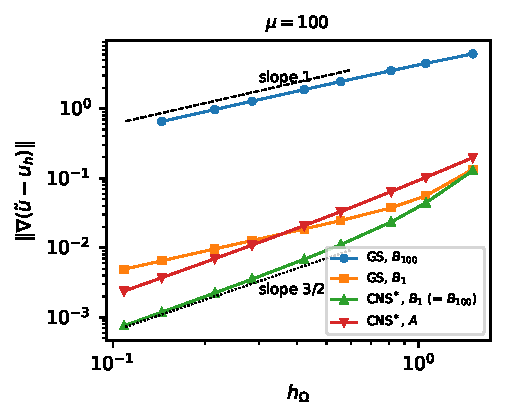
\includegraphics[width=0.48\textwidth]{figures/h1_rates.pdf}\hfill
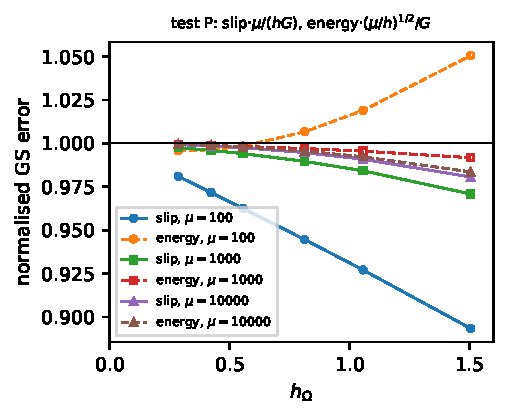
\includegraphics[width=0.48\textwidth]{figures/leading_term.pdf}
\caption{Left: $H^1$ errors at $\mu=100$. $\GS$ has slope $1$ as soon as $G>0$, while $\CNS$ tends to slope $3/2$ independently of the pressure. Right: the normalised slip and energy errors of $\GS$ on test P converge to $1$ (Corollary~\ref{cor:Bp}).}
\label{fig:rates}
\end{figure}

\begin{table}[t]
\centering
\caption{$\CNS$ attains Scott's rate $\hG^{3/2}$ (Theorem~\ref{thm:D}). $H^1$ error, $\mu=100$.}\label{tab:cns}
\begin{tabular}{rrcccc}
\toprule
$N$ & $\hO$ & A & rate & B$_1$ & rate\\
\midrule
32 & 0.813 & $6.41\cdot10^{-2}$ & 1.80 & $2.34\cdot10^{-2}$ & 2.43\\
64 & 0.422 & $2.08\cdot10^{-2}$ & 1.69 & $6.83\cdot10^{-3}$ & 1.76\\
96 & 0.285 & $1.09\cdot10^{-2}$ & 1.64 & $3.54\cdot10^{-3}$ & 1.68\\
128 & 0.215 & $6.96\cdot10^{-3}$ & 1.60 & $2.24\cdot10^{-3}$ & 1.63\\
192 & 0.145 & $3.71\cdot10^{-3}$ & 1.58 & $1.19\cdot10^{-3}$ & 1.60\\
256 & 0.109 & $2.39\cdot10^{-3}$ & 1.56 & $7.58\cdot10^{-4}$ & 1.57\\
\bottomrule
\end{tabular}
\end{table}

\subsection*{Theorem~\ref{thm:D}: $\CNS$}
Table~\ref{tab:cns} gives the $\CNS$ errors. At $N=256$ the energy-norm rate is $1.52$ and the slip rate is $2.02$; the slip carries an extra factor $(h/\mu)^{1/2}$. The $H^1$ rates decrease monotonically toward $3/2$, the geometric term of Lemma~\ref{lem:transposed}. The $\hO^4$ term is invisible at these levels because the geometric term dominates.

The error is independent of the pressure.
\begin{itemize}
\item For polynomial pressures this is structural ($p\in\Pih$). B$_1$ and B$_{100}$ agree to all printed digits wherever both were run ($N\le192$, every $\mu$).
\item With the non-polynomial pressure of test C, the $\CNS$ $H^1$ error differs from that of B$_1$ by a relative $7.9\cdot10^{-7}$, $3.9\cdot10^{-8}$ and $9.7\cdot10^{-9}$ at $N=16$, $64$ and $96$. This is the size of the contribution $\ip{p^\ast-\pi_hp^\ast}{v\cdot n}$, which is of higher order, as Theorem~\ref{thm:D} predicts.
\end{itemize}

\subsection*{Theorems~\ref{thm:A}--\ref{thm:C}: the printed method}
Table~\ref{tab:gs} compares the $H^1$ rates of $\GS$ and $\CNS$ on B$_{100}$.

For the non-polynomial test C at $\mu=100$, the $\GS$ $H^1$ rate from $N=64$ to $96$ is already $1.12$, against $1.68$ for $\CNS$. For the small pressure B$_1$ at $\mu=1000$, $\GS$ still shows $1.51$ at $N=192$. The $(h/\mu)G$ term dominates only once $(h/\mu)G\gtrsim\hG^{3/2}$, which always happens eventually because $\hG^{3/2}$ decays faster. Larger $\mu$ or smaller $G$ delays the crossover but does not remove it.

\begin{table}[t]
\centering
\caption{$\GS$ loses Scott's rate as soon as $G>0$. $H^1$ rate between $N=128$ and $N=192$, test B$_{100}$.}\label{tab:gs}
\begin{tabular}{rcc}
\toprule
$\mu$ & $\GS$ & $\CNS$\\
\midrule
100 & 0.99 & 1.60\\
1000 & 1.00 & 1.56\\
10000 & 1.06 & 1.58\\
\bottomrule
\end{tabular}
\end{table}

\subsection*{Corollary~\ref{cor:Bp}: the leading term}
Table~\ref{tab:P} and Figure~\ref{fig:rates} (right) show the normalised $\GS$ error on test P.
\begin{itemize}
\item The slip and energy ratios converge to $1$. The defect in the slip ratio shrinks with $h/\mu$: at $N=96$ it is $0.019$, $0.0025$ and $0.0007$ for $\mu=10^2$, $10^3$ and $10^4$.
\item The $H^1$ constant is not covered by the corollary. For $\mu=100$ it rises from $2.46$ to $2.71$; for $\mu=10^3$ and $10^4$ it falls, from $2.78$ to $2.77$ and from $3.06$ to $2.79$. This is consistent with a common, $\mu$-independent limit near $2.7$--$2.8$, but the data do not establish one.
\item On test B, $\GS$ itself (B$_1$, $\mu=100$, $N=256$) gives slip and energy ratios $0.995$ and $1.001$.
\item For $\mu=10^4$ with the small pressure B$_1$, $\gamma\hG\approx74\gg G$ at $N=192$, so the hypothesis of the corollary fails. The $\GS$ energy ratio there is about $7.8$, dominated by the geometric error rather than the traction response.
\item The difference $u_{\GS}-u_{\CNS}$ is not a clean proxy for the traction response on test B. It also contains the difference between the two methods on the velocity part, which is $O(\hG^{3/2})$ and non-zero even for test A. Test P removes this.
\end{itemize}

\begin{table}[t]
\centering
\caption{The leading term of Corollary~\ref{cor:Bp}. Normalised $\GS$ error on test P ($G=1.658$), where $e=\ut-u_h$.}\label{tab:P}
\begin{tabular}{rrccc}
\toprule
$N$ & $\mu$ & $\norm{\nabla e}\,\mu/(hG)$ & $\norm{e}_{\Gh}\,\mu/(hG)$ & $\tnorm{e}(\mu/h)^{1/2}/G$\\
\midrule
16 & 100 & 2.464 & 0.894 & 1.051\\
32 & 100 & 2.612 & 0.945 & 1.007\\
64 & 100 & 2.684 & 0.972 & 0.996\\
96 & 100 & 2.708 & 0.981 & 0.996\\
96 & 1000 & 2.770 & 0.998 & 0.999\\
96 & 10000 & 2.790 & 0.9993 & 0.9994\\
\bottomrule
\end{tabular}
\end{table}

\subsection*{Proposition~\ref{prop:penalty}: the penalty study}
The coercivity threshold $\mu^\ast$ on $\Zh$ is the smallest $\mu$ for which the unpivoted symmetric factorisation of $A_\mu+rB^{\mathsf T}M^{-1}B$ has only positive pivots; we locate it by bisection. Table~\ref{tab:thresh} and Figure~\ref{fig:thresh} show the results.

Under refinement at fixed $\rho$, $\gamma^\ast$ increases by $3.4$ ($N=8\to16$), $1.8$ ($16\to32$) and $0.95$ ($32\to64$). The increments roughly halve, which suggests, but does not prove, a limit near $22$.

In part (b) of Table~\ref{tab:thresh}, $\rho$ is varied by coarsening the far field while the boundary layer is held fixed. Then $\mu^\ast$ is linear in $\rho$ over more than a decade, with a constant slope. The threshold is thus set locally at $\Gh$ ($\mu/h\gtrsim c/\hG$), and the $\rho$-scaling is the cost of normalising the penalty by the global $h$.

In practical terms:
\begin{itemize}
\item a safe choice is $\mu\ge25\rho$, that is, $\gamma\ge25$;
\item a fixed $\mu$ fails once the far field is coarsened beyond $\rho\approx\mu/20$.
\end{itemize}
The exact certificate $\lambda\ge9$ on $\cS_3$ and $\cS_4'$ is a local lower bound, consistent with the global $\gamma^\ast\approx18$--$21$.

\begin{table}[t]
\centering
\caption{Coercivity threshold $\mu^\ast$ and $\gamma^\ast=\mu^\ast/\rho$.}\label{tab:thresh}
\small
\textit{(a) Refinement at fixed $\rho$.}\\[2pt]
\begin{tabular}{lcccccccc}
\toprule
$N$ & 8 & 12 & 16 & 20 & 24 & 32 & 48 & 64\\
\midrule
$\rho$ & 3.41 & 3.02 & 3.28 & 3.17 & 3.30 & 3.33 & 3.37 & 3.40\\
$\mu^\ast$ & 50.3 & 51.8 & 59.3 & 60.3 & 63.3 & 66.0 & 69.1 & 70.7\\
$\gamma^\ast$ & 14.7 & 17.1 & 18.1 & 19.1 & 19.2 & 19.9 & 20.5 & 20.8\\
\bottomrule
\end{tabular}\\[6pt]
\textit{(b) Varying $\rho$ through the outer box $(-L,L)^2$.}\\[2pt]
\begin{tabular}{llccccc}
\toprule
 & $L$ & 2.5 & 5 & 10 & 20 & 40\\
\midrule
$N=16$ & $\rho$ & 3.28 & 5.90 & 11.3 & 22.2 & 43.9\\
 & $\mu^\ast$ & 59.3 & 112.1 & 208.0 & 411.5 & 809.3\\
 & $\gamma^\ast$ & 18.1 & 19.0 & 18.4 & 18.5 & 18.4\\
\midrule
$N=32$ & $\rho$ & 3.33 & 5.79 & 10.8 & 21.1 & 41.5\\
 & $\mu^\ast$ & 66.0 & 113.9 & 218.0 & 422.2 & 835.7\\
 & $\gamma^\ast$ & 19.9 & 19.7 & 20.1 & 20.0 & 20.1\\
\bottomrule
\end{tabular}
\end{table}

\begin{figure}[t]
\centering
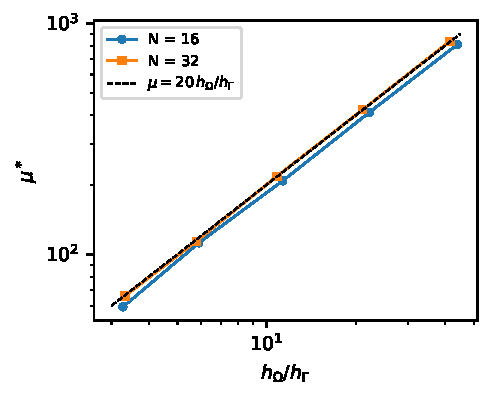
\includegraphics[width=0.48\textwidth]{figures/threshold.pdf}
\caption{Coercivity threshold $\mu^\ast$ against $\rho$ (Table~\ref{tab:thresh}(b)).}
\label{fig:thresh}
\end{figure}

\subsection*{Lemma tests}
We compute exact discrete dual norms, $\sup_v\ell(v)/\norm{\nabla v}$ over $\Zh$ or $\VR$, by a saddle-point solve with the pointwise divergence constraint. Table~\ref{tab:lemma} gives the rates for $N=48\to64$.
\cert{code/lemma\_tests.py 16,24,32,48,64}{logs/lemma\_tests.log}

\begin{table}[t]
\centering
\caption{Exact discrete dual norms; rate in $\hG$ for $N=48\to64$ (positive means decay).}\label{tab:lemma}
\begin{tabular}{llc}
\toprule
Functional & Space & Rate\\
\midrule
$\ip{S}{\dn v}$, $S$ normal & $\Zh$ & $+0.05$ (bounded, $\approx1.75$)\\
$\ip{S}{\dn v}$, $S$ normal & $\VR$ & $-0.52$\\
$\ip{S}{\dn v}$, $S$ tangential & $\Zh$ & $-0.52$\\
$\ip{(\nabla\ut)^{\mathsf T}n}{v}$, tests A / B & $\VR$ & $1.57$ / $1.56$ (Lemma~\ref{lem:transposed}: $3/2$)\\
\bottomrule
\end{tabular}
\end{table}


\appendix
\section{Reproducibility}\label{app:repro}

All code, raw outputs and logs are in the repository that accompanies this paper. Paths below are relative to its root; commands are run from \texttt{code/}. \texttt{code/regen\_logs.sh} regenerates every log in \texttt{logs/} with the commands below, and \texttt{make report} checks that all three reports are reproduced byte-for-byte.

\subsection*{Code (\texttt{code/})}
\begin{itemize}
\item \texttt{svn.py}: the solver. It contains the mesh generator, the $P_4$ space, assembly of $N_h$, $B$ and the $\CNS$ coupling, the SuperLU saddle-point solver (\texttt{solve\_lu}), error norms, and the exact solutions for tests A, B, P and C.
\item \texttt{job.py}: one study or threshold job per process.
\item \texttt{run\_all.py}: memory- and CPU-aware scheduler for the full campaign.
\item \texttt{report.py} and \texttt{report\_local.py}: produce the tables.
\item \texttt{plots.py}: produces the figures.
\item \texttt{penalty.py}: computes the coercivity threshold $\mu^\ast$.
\item \texttt{lemma\_tests.py}: computes the dual norms of Table~\ref{tab:lemma}.
\item \texttt{lamstar\_exact.py} and \texttt{lamstar\_exact\_v2.py}: the exact certificates of Proposition~\ref{prop:penalty}.
\item \texttt{lamstar.py}: the floating-point $\lambda^\ast$ on other fans.
\end{itemize}
Added in this version:
\begin{itemize}
\item \texttt{svn\_k.py}: degree-general solver ($P_k$ velocities, $k\ge2$; standard or Clough--Tocher mesh; SuperLU or PARDISO). \texttt{job\_k.py} runs one study or threshold job, \texttt{penalty\_k.py} computes $\mu^\ast$, \texttt{report\_v3.py} writes the tables, and \texttt{validate\_k.py} checks $k=4$ against \texttt{svn.py} and PARDISO against SuperLU. The scheduler is \texttt{results/v3/sched.py}, with job list \texttt{results/v3/jobs.txt}.
\item \texttt{lamstar\_exact\_ct.py}: the exact local-surjectivity ranks and penalty certificates on Clough--Tocher stars (Section~\ref{ct:sec}).
\item \texttt{lamstar\_family.py}: the single-triangle forms, the shape-family certificates and the patch thresholds (Section~\ref{pb:sec}).
\item \texttt{h1\_limit.py}: the annulus bracket, the series solution and the finite element comparison for the $H^1$ constant (Section~\ref{hc:sec}).
\item \texttt{lower\_bound\_tests.py}: the (M3) star constants, the assembled test field and the dual norms (Section~\ref{lb:sec}).
\item \texttt{plot\_leak.py}: Figure~\ref{fig:leak}.
\item \texttt{notes/v3/face\_mean\_check.py}: the face-mean check of Lemma~\ref{td:faces}(d).
\end{itemize}

\subsection*{Where each number comes from}
\begin{center}
\small
\begin{tabular}{>{\raggedright\arraybackslash}p{0.24\textwidth}>{\raggedright\arraybackslash}p{0.36\textwidth}>{\raggedright\arraybackslash}p{0.34\textwidth}}
\toprule
Result & Command & Output\\
\midrule
Tables~\ref{tab:cns}, \ref{tab:gs}, \ref{tab:thresh} & \texttt{SVN\_OUT=../results/pod python3 run\_all.py}, then \texttt{python3 report.py ../results/pod} & \texttt{results/pod/report.txt}\\
Table~\ref{tab:P}, test C & \texttt{SVN\_OUT=../results/local python3 job.py study N P1 MU} and \texttt{SVN\_OUT=../results/local python3 job.py study N C 100}, then \texttt{python3 report\_local.py} & \texttt{results/local/report\_local.txt}\\
Certificate for $\cS_3$ & \texttt{python3 lamstar\_exact.py} & \texttt{logs/lamstar\_exact\_\allowbreak S3\_S4singular.log}\\
Certificate for $\cS_4'$ & \texttt{python3 lamstar\_exact\_v2.py} & \texttt{logs/lamstar\_exact\_S4prime.log}\\
Table~\ref{tab:lemma} & \texttt{python3 lemma\_tests.py 16,24,32,48,64} & \texttt{logs/lemma\_tests.log}\\
Floating-point $\lambda^\ast$ & \texttt{python3 -W ignore::DeprecationWarning lamstar.py} & \texttt{logs/lamstar\_float.log}\\
Figures~\ref{fig:rates}, \ref{fig:thresh} & \texttt{python3 plots.py} & \texttt{paper/figures/}\allowbreak\texttt{h1\_rates.pdf} etc.\\
Figure~\ref{fig:leak} & \texttt{python3 plot\_leak.py} & \texttt{paper/figures/}\allowbreak\texttt{leak\_field.pdf}\\
Tables~\ref{tab:threshv3}--\ref{tab:ratesv3} & \texttt{SVN\_SOLVER=pardiso python3 ../results/v3/sched.py ../results/v3/jobs.txt LOG} (runs \texttt{job\_k.py}; output root \texttt{results/v3} by default, or \texttt{SVN\_OUT}), then \texttt{python3 report\_v3.py} & \texttt{results/v3/}\allowbreak\texttt{report\_v3.txt}\\
Validation of \texttt{svn\_k.py} & \texttt{python3 validate\_k.py} & \texttt{results/v3/}\allowbreak\texttt{validation.txt}\\
Lemma~\ref{ct:lem:local} ($k=3$), Table~\ref{ct:tab:lam} & \texttt{python3 lamstar\_exact\_ct.py} & \texttt{logs/lamstar\_}\allowbreak\texttt{exact\_ct.log}\\
Theorem~\ref{pb:thm}, Proposition~\ref{pb:cert} & \texttt{python3 lamstar\_family.py bubble}; \texttt{\ldots\ certify} & \texttt{logs/lamstar\_family\_}\allowbreak\texttt{bubble.log}, \texttt{\ldots\_certify.log}\\
Patch thresholds (Section~\ref{pb:sec}) & \texttt{python3 lamstar\_family.py mesh}; \texttt{\ldots\ limit}; \texttt{\ldots\ limitstar} & \texttt{logs/lamstar\_family\_}\allowbreak\texttt{mesh.log}, \texttt{\ldots\_limit.log}, \texttt{\ldots\_limitstar.log}\\
Level-set and tall-triangle values of $\lambda_T$ (Section~\ref{pb:sec}) & \texttt{python3 lamstar\_family.py levels} & \texttt{logs/lamstar\_family\_}\allowbreak\texttt{levels.log}\\
$H^1$ constant (Section~\ref{hc:sec}) & \texttt{python3 h1\_limit.py annulus} and \texttt{\ldots\ mps} (series log); \texttt{\ldots\ fem} & \texttt{logs/h1\_limit\_}\allowbreak\texttt{series.log}, \texttt{\ldots\_fem.log}\\
(M3) and Tables~\ref{lb:tab:stars}, \ref{lb:tab:field} & \texttt{python3 lower\_bound\_tests.py} with \texttt{stars 8,12,\ldots,1024}, \texttt{field 16,\ldots,512}, \texttt{global 16,\ldots,64} & \texttt{logs/lower\_bound\_}\allowbreak\texttt{stars.log}, \texttt{\ldots\_field.log}, \texttt{\ldots\_global.log}\\
Lemma~\ref{td:faces}(d) & \texttt{python3 notes/v3/}\allowbreak\texttt{face\_mean\_check.py} (from the root) & standard output\\
\bottomrule
\end{tabular}
\end{center}

\subsection*{Resources}
The full A/B campaign (74 study jobs up to $N=256$ and 16 threshold jobs) took 36 minutes on 32 cores with 125\,GB of memory. The largest single job ($N=256$, both methods) takes about 23 minutes; the scheduler reserved up to 55\,GB for it. Every job with $N\le96$ runs on a 2-core, 7\,GB machine.

The runs of Section~\ref{sec:numv3} used a 2-core machine with a 5.8\,GB memory limit shared with other jobs; the largest single job used 3.6\,GB (peak RSS is recorded in each record). Each job took at most about $2.5$ minutes.

The environment was Python 3.11 with NumPy 2.4, SciPy 1.17 (SuperLU) and SymPy 1.14. The runs of Section~\ref{sec:numv3} also used MKL PARDISO through \texttt{pypardiso}.


\section*{Use of generative-AI tools declaration}
The author used Anthropic's Claude Opus~5.5 as a research-support tool. It assisted with the following:
\begin{itemize}
\item developing and checking the proofs;
\item implementing, running and validating the finite element code and the exact-arithmetic certificates;
\item independently reviewing the arguments as a referee;
\item preparing the manuscript and the accompanying repository.
\end{itemize}
The author directed the project and retains authorship of the work. Responsibility for all mathematical statements, computations, references and conclusions rests with the author.


\bibliographystyle{amsplain}
\bibliography{refs}

\end{document}
